\chapter{Anéis}

\section{Conceitos básicos}

\subsection{Anel e subanel}

\begin{definition}
Um \emph{anel} é uma lista $\bm A=(A,+,-,0,\times,1)$ tal que
	\begin{enumerate}
	\item $\bm A^+ := (A,+,-,0)$ é um grupo comutativo, em que $+$ é a \emph{adição}, $-$ é a \emph{inversão aditiva} e $0$ é a \emph{nulidade} (ou o \emph{zero}) de $\bm A$;
	\item $\bm A^\times := (A,\times,1)$ é um monoide comutativo, em que $\times$ é a \emph{multiplicação} e $1$ é a \emph{unidade} (ou o \emph{um}) de $\bm A$;
	\item A multiplicação $\times$ é distributiva sobre a adição $+$.
	\end{enumerate}
% A imagem de dois elementos $a_1,a_2 \in A$ pela adição é chamada de \emph{soma} de $a_1$ e $a_2$ e denotada por $a_1+a_2$. A imagem de $a_1,a_2$ pela multiplicação é chamada de \emph{produto} de $a_1$ e $a_2$ e denotada por $a_1 \cdot a_1$ ou $a_1a_2$.
\end{definition}

%\begin{definition}
%	Um \emph{anel} é uma tripla $\bm A=(A,+,\cdot)$ em que
%	\begin{enumerate}
%	\item $(A,+)$ é um grupo comutativo com elemento neutro chamado de \emph{zero} ou \emph{nulidade} e representado por $0$ (ou $0_A$, caso exista ambiguidade).
%	\item $(A,\cdot)$ é um monoide comutativo com elemento neutro chamado de \emph{um} ou \emph{unidade} e representado por $1$ (ou $1_A$, caso exista ambiguidade).
%	\item A operação $\cdot$ é distributiva sobre $+$.
%	\end{enumerate}
%As operações $+$ e $\cdot$ são chamadas, respectivamente, de \emph{adição} e \emph{multiplicação}. A imagem de dois elementos $a_1,a_2 \in A$ pela adição é chamada de \emph{soma} de $a_1$ e $a_2$ e denotada por $a_1+a_2$. A imagem de $a_1,a_2$ pela multiplicação é chamada de \emph{produto} de $a_1$ e $a_2$ e denotada por $a_1 \cdot a_1$ ou $a_1a_2$.
%\end{definition}
\begin{notation}
O símbolo de multiplicação $\times$ será suprimido sempre que possível, de modo que denotaremos $a_0a_1$ para $a_0 \times a_1$, e a notação da multiplicação terá preferência sobre a da adição e a da substração, pois $\times$ é distributiva sobre $+$, de modo que denotaremos $a_0a_1 + a_2$ para $(a_1a_2) + a_3$ e $-a_1a_2$ para $-(a_1a_2)$. Os símbolos operatórios relativos à adição e à multiplicação serão, respectivamente,
	\begin{equation*}
	\sum \text{\ \ e\ \ } \bigtimes.
	\end{equation*}
O elemento $a$ multiplicado por si mesmo $n$ vezes será denotado $a^n$. Denotaremos o inverso de um elemento $a \in A$ com respeito a $\times$ por $a\inv$ ou $\div a$, se ele existir, pois sabemos que é único (\ref{prop:unic.inv}).
\end{notation}

%\begin{notation}
%Como $(A,+)$ é um grupo, denotaremos o inverso de um elemento $a \in A$ sob $+$ por $-a$, e escreveremos $a_1 - a_2$ para $a_1 + (-a_2)$. Ainda, a multiplicação tem preferência na notação; ou seja, $a_1a_2+a_3 = (a_1 \cdot a_2)+a_3$ e $-a_1a_2 = -(a_1 \cdot a_2)$. Denotaremos o inverso de um elemento $a \in A$ sob $\cdot$ por $a^{-1}$, se ele existir, pois sabemos que é único (\ref{prop:unic.inv}). Os símbolos operatórios relativos à adição e à multiplicação serão, respectivamente, $\sum$ e $\bigtimes$. Caso não haja ambiguidade, denotaremos um anel pelo símbolo que denota seu conjunto escrito em negrito, como em $\bm A=(A,+,\cdot)$.
%\end{notation}

Na definição de anel aqui adotada, consideramos anéis que têm multiplicação comutativa e unidade. Em contextos mais gerais, esses objetos são chamados de \emph{anéis comutativos unitários}.

Um comentário sobre as identidades $0$ e $1$. Se $0=1$, o anel será \emph{trivial}, no sentido de que $0$ será seu único elemento, mas mantemos esse caso na definição pois, mais à frente, no estudo de anéis quocientes, será proveitoso que qualquer anel quociente seja um anel, e o quociente de um anel por ele mesmo é o anel trivial.


\begin{proposition}
Seja $\bm A$ um anel. Então, para todos $a,a' \in A$,
	\begin{enumerate}
	\item $0a = 0$;
	\item Se $0=1$, então $A=\{0\}$;
	\item $-(aa') = (-a)a'$.
	\end{enumerate}
\end{proposition}
\begin{proof}
	\begin{enumerate}
	\item
%		\begin{align*}
%		0 \cdot a &= 0 \cdot a + 0 \\
%			&= 0 \cdot a + (0 \cdot a - 0 \cdot a) \\
%			&= (0 \cdot a + 0 \cdot a) - 0 \cdot a \\
%			&= (0+0) \cdot a - 0 \cdot a \\
%			&= 0 \cdot a - 0 \cdot a \\
%			&= 0.
%		\end{align*}
		\begin{align*}
		0 a &= 0 a + 0 \\
			&= 0 a + (0 a - 0 a) \\
			&= (0 a + 0 a) - 0 a \\
			&= (0+0) a - 0 a \\
			&= 0 a - 0 a \\
			&= 0.
		\end{align*}
	
	\item Se $0=1$, então, para todo $a \in A$,
		\begin{equation*}
		a = 1a = 0a = 0;
		\end{equation*}	
	
	\item
%		\begin{align*}
%		-(a \cdot b) &= -(a \cdot b) + 0 \\
%			&= -(a \cdot b) + 0 \cdot b \\
%			&= -(a \cdot b) + (a - a) \cdot b \\
%			&= -(a \cdot b) + (a \cdot b + (-a) \cdot b) \\
%			&= (-(a \cdot b) + a \cdot b) + (-a) \cdot b \\
%			&= 0 + (-a) \cdot b \\
%			&= (-a) \cdot b.
%		\end{align*}
		\begin{align*}
		-(a a') &= -(a a') + 0 \\
			&= -(a a') + 0 a' \\
			&= -(a a') + (a - a) a' \\
			&= -(a a') + (a a' + (-a) a') \\
			&= (-(a a') + a a') + (-a) a' \\
			&= 0 + (-a) a' \\
			&= (-a) a'.
		\end{align*}
	\end{enumerate}
\end{proof}

\begin{definition}
Seja $\bm A$ um anel. O conjunto dos elementos invertíveis sob multiplicação de $\bm A$ é denotado por $A^*$.
\end{definition}

\begin{proposition}
Seja $\bm A$ um anel. A lista $(A^*,\times|_{A^* \times A^*},\div,1)$ é um grupo comutativo.
\end{proposition}
\begin{proof}
A tripla $(A,\times,1)$ é um monoide comutativo com identidade $1$. Portanto segue que a quádrupla $(A^*,\times|_{A^* \times A^*},\div,1)$ é um grupo (em que $\div a = a\inv$ denota o inverso de $a$ sob $\times$). Como $\times$ é comutativa, então $(A^*,\times|_{(A^*)^2},\inv,1)$ também o é.
\end{proof}

\begin{definition}
Seja $\bm A=(A,+,-,0,\times,1)$ um anel. Um \emph{subanel} de $\bm A$ é um anel $\bm S=(S,+_S,-_{S},0_S,\times_S,1_S)$ tal que $S \subseteq A$, $+_S = +|_{S \times S}$, $-_S = -|_{S}$, $0_S=0$, $\times_S = \times|_{S \times S}$ e $1_S=1$. Denota-se $\bm S \leq \bm A$. Um subanel \emph{próprio} de $\bm A$ é um subanel $\bm S \leq \bm A$ em que $S$ é um conjunto próprio de $A$ ($S \subset A$). Denota-se $\bm S < \bm A$.
\end{definition}

\begin{proposition}
Sejam $\bm A=(A,+,-,0,\times,1)$ um anel e $S \subseteq A$. Então
	\begin{equation*}
	\bm S=(S,+|_{S \times S},-|_{S},0,\times|_{S \times S},1)
	\end{equation*}
é um anel se, e somente se,
	\begin{enumerate}
	\item $\bm S^+ = (S,+|_{S \times S},-|_{S},0)$ é um subgrupo comutativo de $\bm A^+$
			\begin{enumerate}
			\item [\ref{SG1}] (Não-vacuidade) $S \neq \emptyset$;
			\item [\ref{SG2}] (Fechamento) Para todos $s_1,s_2 \in S$, $s_1 + s_2 \in S$;
			\item [\ref{SG3}] (Invertibilidade) Para todo $s \in S$, $-s \in S$;
			\end{enumerate}
	\item $\bm S^\times = (S,\times|_{S \times S},1)$ é um submonoide comutativo de $\bm A^\times$
			\begin{enumerate}
			\item [\ref{SM1}] (Identidade) $1 \in S$;
			\item [\ref{SM2}] (Fechamento) Para todos $s_1,s_2 \in S$, $s_1 \times s_2 \in S$.
			\end{enumerate}
	\end{enumerate}
\end{proposition}
\begin{proof}
	\begin{itemize}
	\item [($\Rightarrow$)] Suponhamos que $\bm S$ é um anel.
		\begin{enumerate}
		\item (Subgrupo) Como $S \subseteq A$ e $\bm S^+$ um grupo comutativo, então é um subgrupo de $\bm A^+$ por definição de subgrupo (o que é equivalente às propriedades listadas) e é comutativo (\ref{alge:prop.subgru})).
		
		\item (Submonoide) Como $S \subseteq A$ e $\bm S^\times$ é um monoide comutativo com $1 \in S$, então é um submonoide de $(A,\times)$ por definição de submonoide (o que é equivalente às propriedades listadas) e é comutativo (\ref{alge:prop.submon}).
		\end{enumerate}

	\item [($\Leftarrow$)] Suponhamos, agora, que $\bm S^+$ é subgrupo comutativo de $\bm A^+$ e $\bm S^\times$ é submonoide comutativo de $\bm A^\times$.
		\begin{enumerate}
		\item (Grupo comutativo) Como $(S,+|_{S \times S})$ é subgrupo comutativo, então é um grupo comutativo por definição de subgrupo.
		
		\item (Monoide comutativo) Como $(S,\times|_{S \times S})$ é submonoide comutativo, então é um monoide comutativo por definição de monoide.
		
		\item (Distributividade) Sejam $s_1,s_2,s_3 \in S$. Então
	\begin{align*}
	s_1 \mathrel{\times|_{S \times S}} (s_2 \mathrel{+|_{S \times S}} s_3) &= s_1 \times (s_2 + s_3) \\
		&= (s_1 \times s_2) + (s_1 \times s_3) \\
		&= (s_1 \mathrel{\times|_{S \times S}} s_2) \mathrel{+|_{S \times S}} (s_1 \mathrel{\times|_{S \times S}} s_3).
	\end{align*}
Logo $\times_{S \times S}$ é distributiva sobre $+ \times_{S \times S}$.
		\end{enumerate}
	\end{itemize}
\end{proof}

\subsection{Ideais e anéis quocientes}

\begin{definition}
Seja $\bm A$ um anel. Um \emph{ideal} de $\bm A$ é um conjunto não vazio $I \subseteq A$ tal que
	\begin{enumerate}
	\item Para todos $i_1,i_2 \in I$, $i_1 - i_2 \in I$;
	\item Para todos $a \in A$ e $i \in I$, $ai \in I$.
	\end{enumerate}
Denotamos que $I$ é ideal de $\bm A$ por $I \ide A$. Ainda, $I \idepro A$ significa que $I \neq A$ e $I \ide A$.
\end{definition}

É interessante observar que $I$ é subgrupo de $(A,+)$. A definição de ideal difere da definição de subanel na propriedade 2.

\begin{proposition}
Sejam $\bm A$ um anel e $I \ide A$. Então
	\begin{enumerate}
	\item $0 \in I$;
	\item Para todos $i_1,i_2 \in I$, $i_1 + i_2 \in I$;
	\item $1 \in I \Rightarrow I=A$;
	\item $\{0\}$ e $A$ são ideais de $A$.
	\end{enumerate}
\end{proposition}
\begin{proof}
	\begin{enumerate}
	\item Seja $i \in I$. Então $0 = i-i \in I$.
	\item Sejam $i_1,i_2 \in I$. Pelo item anterior, sabemos que $0 \in I$, o que implica $-i_2 = 0 - i_2 \in I$. Logo $i_1 + i_2 = i_1 - (-i_2) \in I$.
	\item Se $1 \in I \ide A$, então, para todo $a \in A$, temos $a=a\cdot1 \in A$. Logo $I=A$.
	\item Consideremos $\{0\}$. Se $i \in \{0\}$, então $i=0$. Portanto, para todo $a \in A$ e $i \in \{0\}$, temos $i-i=0 \in \{0\}$ e $ai=0 \in \{0\}$. Logo $\{0\} \ide A$. Agora, consideremos $A$. Para todo $a_1,a_2 \in A$, temos $a_1-a_2 \in A$ e $a_1a_2 \in A$. Logo $A \ide A$.
	\end{enumerate}
\end{proof}

\begin{proposition}
Sejam $\bm A$ um anel e $(I_j)_{j \in J}$ uma família de ideais de $\bm A$. Então
	\begin{equation*}
	I := \bigcap_{j \in J} I_j
	\end{equation*}
é um ideal de $\bm A$.
\end{proposition}
\begin{proof}
	Sejam $i_1,i_2 \in I$ e $a \in A$. Então, para todo $j \in J$, $i_1,i_2 \in I_j$ e, como $I_j$ é ideal de $\bm A$, segue que $i_1-i_2 \in I_j$ e que $ai_1 \in W_i$. Logo $i_1-i_2 \in I$ e $ai_1 \in I$, o que mostra que $I$ é ideal de $\bm A$.
\end{proof}

\begin{proposition}
	Sejam $\bm A$ um anel e $(I_j)_{n \in \N}$ uma sequência crescente de ideais de $\bm A$; ou seja, $I_1 \subseteq I_2 \subseteq \cdots \subseteq I_n \subseteq \cdots$. Então
	\begin{equation*}
	I := \bigcup_{n \in \N} I_n
	\end{equation*}
é um ideal de $\bm A$.
\end{proposition}
\begin{proof}
	Sejam $i_1,i_2 \in I$. Então existem $n,m \in \N$ tais que $i_1 \in I_n$ e $i_2 \in I_m$. Nesse caso, $I_n \subseteq I_m$ ou $I_m \subseteq I_n$. Sem perda de generalidade, suponhamos o primeiro caso. Então segue que $i_1 \in I_m$ e, portanto, $i_1-i_2 \in I_m$, o que mostra que $i_1-i_2 \in I$. Agora, seja $a \in A$ e notemos que, como $I_n$ é ideal de $\bm A$, segue que $ai_1 \in I_n$. Logo $ai_1 \in I$, o que mostra que $I$ é ideal de $\bm A$.
\end{proof}

Lembremos, dados $\bm A$ um anel e $a_1,\ldots,a_n \in A$, definimos o conjunto
	\begin{equation*}
	\sum_{i=1}^n a_iA = a_1A + \ldots + a_nA = \set{\sum_{i=1}^n a_ib_i}{b_i \in A}.
	\end{equation*}

\begin{proposition}
Sejam $\bm A$ um anel e $a_1,\ldots,a_n \in A$. Então
	\begin{equation*}
	I := \sum_{k=1}^n a_kA \ide A.
	\end{equation*}
\end{proposition}
\begin{proof}
	Sejam $a \in A$ e $i_1,i_2 \in I$ tais que $i_1=\sum_{k=1}^n a_ib_i$ e $i_2=\sum_{k=1}^n a_ic_i$. Então
	\begin{equation*}
	i_1-i_2=\sum_{k=1}^n a_kb_k - \sum_{k=1}^n a_kc_k = \sum_{k=1}^n a_k(b_k-c_k) \in I,
	\end{equation*}
pois $(b_k-c_k) \in A$ para todo $k \in \{1,\ldots,n\}$. Ainda,
	\begin{equation*}
	ak_1=a\sum_{k=1}^n a_kb_k= \sum_{k=1}^n a_k(ab_k) \in I,
	\end{equation*}
pois $ab_k \in A$ para todo $k \in \{1,\ldots,n\}$. Logo $I \ide A$.
\end{proof}

Esse ideal é chamado de ideal de $A$ gerado por $a_1,\ldots,a_n$.

\begin{definition}
Seja $\bm A$ um anel. Um \emph{ideal principal} de $\bm A$ é um ideal $I \ide A$ tal que, para algum $a \in A$, $I=aA$.
\end{definition}

\begin{proposition}
\label{pro:corp.sse.ide}
	Seja $\bm A$ um anel. Então $\bm A$ é um corpo se, e somente se, é um anel não-trivial cujos únicos ideais são $\{0\}$ e $A$.
\end{proposition}
\begin{proof}
	Suponha que $\bm A$ é um corpo. Então $(A\setminus\{0\},\cdot)$ é um grupo e, portanto, $A \neq \emptyset$. Seja $I \ide A$ e suponha que $I \neq \{0\}$. Então existe $i \in I\setminus\{0\}$. Como $\bm A$ é corpo, existe $i^{-1} \in A$. Portanto $1=i^{-1}i \in I$. Logo $I=A$.

	Por outro lado, suponha que os únicos ideais de $A$ são $\{0\}$ e $A$. Como $\bm A$ é não-trivial, seja $a \in A\setminus\{0\}$ e consideremos o ideal $I=aA$. Notemos que $a=a \cdot 1 \in aA$, o que implica $I \neq \{0\}$. Portanto $I=A$. Mas então $1 \in aA$, o que significa que deve existir $b \in A$ tal que $1=ab$; ou seja, todo $a \in A\setminus\{0\}$ tem inverso em $A$. Logo $\bm A$ é corpo.
\end{proof}

\begin{proposition}
	Sejam $\bm A$ um anel e $I \ide A$. A relação binária $\sim_I$ em $A$, definida por
	\begin{equation*}
	a \sim_I b \Leftrightarrow a-b \in I,
	\end{equation*}
é uma relação de equivalência.
\end{proposition}
\begin{proof} Vamos demonstrar as três propriedades de uma relação de equivalência.
	\begin{enumerate}
	\item (Reflexividade) Seja $a \in A$. Então $a-a=0 \in I$. Logo $a \sim_I a$.
	\item (Simetria) Sejam $a_1,a_2 \in A$ tais que $a_1 \sim_I a_2$. Então $(a_1-a_2) \in I$. Mas $0 \in I$, o que implica $a_2-a_1 = 0-(a_1-a_2) \in I$. Logo $a_2 \sim_I a_1$.
	\item (Transitividade) Sejam $a_1,a_2,a_3 \in A$ tais que $a_1 \sim_I a_2$ e $a_2 \sim_I a_3$. Então $(a_1-a_2),(a_2-a_3) \in I$, o que implica $a_1-a_3=(a_1-a_2)+(a_2-a_3) \in I$. Logo $a_1 \sim_I a_3$.
	\end{enumerate}
\end{proof}

\begin{definition}
Sejam $\bm A$ um anel e $I \ide A$. O conjunto $a+I = \set{a+i}{i \in I}$ é a \emph{classe lateral} de $I$ e $a$ é um \emph{representante} da classe. O conjunto das classes laterais de $A$ é denotado por $\quo{A}{I} := \set{a+I}{a \in A}$.
\end{definition}

\begin{proposition}
Sejam $(A,+,\cdot)$ um anel, $I \ide A$ e $\sim_I$ a relação de equivalência definida na proposição anterior e $a \in A$. Então a classe de equivalência $[a]=\set{b \in A}{b \sim_I a}$ é igual à classe lateral $a+I$ e, por consequência, o conjunto quociente $\quo{A}{\sim_I}$ é igual ao conjunto $\quo{A}{I}$.
\end{proposition}
\begin{proof}
Seja $b \in [a]$. Então $b-a \in I$; ou seja, existe $i \in I$ tal que $b-a=i$. Mas isso implica $b=a+i$, que implica, por sua vez, que $b \in a+I$. Por outro lado, seja $b \in a+I$. Então existe $i \in I$ tal que $b=a+i$; ou seja, $b-a=i$, que implica $b-a \in I$ e, assim, $b \in [a]$. Disso, vem que $A/\sim_I = A/I$.
\end{proof}

Uma consequência disso é que o conjunto $A$ é particionado em classes laterais de $I$. Outra consequência é que duas classes laterais são iguais se, e somente se, a diferença entre seus representantes está em $I$.

\begin{definition}
Sejam $\bm A$ um anel, $I \ide A$ e $a_1,a_2 \in A$. Então definimos as operações binárias $\oplus$ e $\odot$ em $A/I$ por
	\begin{equation*}
	(a_1+I) \oplus (a_2+I) := (a_1+a_2)+I \qquad \qquad (a_1+I) \odot (a_2+I) := (a_1 \cdot a_2)+I
	\end{equation*}
Denotaremos $\oplus$ e $\odot$ por $+$ e $\cdot$ quando não existir ambiguidade.
\end{definition}

\begin{proposition}
As operações $\oplus$ e $\odot$ da definição anterior estão bem definidas.
\end{proposition}
\begin{proof}
	Sejam $a_1,a_2,b_1,b_2 \in A$ tais que $a_1+I=a_2+I$ e $b_1+I=b_2+I$. Primeiro, vamos mostrar que $\oplus$ está bem definida. Devemos mostrar que $(a_1+b_1)+I=(a_2+b_2)+I$. De $a_1+I=a_2+I$, sabemos que $a_1-a_2 \in I$. Da mesma forma, $b_1-b_2 \in I$. Mas então $(a_1+b_1)-(a_2+b_2) = (a_1-a_2)+(b_1-b_2) \in I$, o que implica $(a_1+b_1)+I=(a_2+b_2)+I$.

	Agora, vamos mostrar que $\odot$ está bem definida. Devemos mostrar que $(a_1b_1)+I=(a_2b_2)+I$. Sejam $c=a_1-a_2$ e $d=b_1-b_2$. Notemos que
	\begin{equation*}
	a_1b_1 = (a_2+c)(b_2+d) = a_2b_2 + a_2d + cb_2 + cd.
	\end{equation*}
Como $c,d \in I$, $(a_2d + cb_2 + cd) \in I$. Logo $a_1b_1-a_2b_2 \in I$, o que implica $(a_1b_1)+I=(a_2b_2)+I$.
\end{proof}

\begin{proposition}
	Sejam $\bm A=(A,+,\cdot)$ um anel e $I \ide A$. Então $\bm{A/I} := (A/I,\oplus,\odot)$ é um anel, chamado \emph{anel quociente} de $A$ por $I$.
\end{proposition}
\begin{proof}
	Sejam $a_1,a_2,a_3 \in A$. Primeiro, vamos mostrar que $(A/I,\oplus)$ é um grupo comutativo. As propriedades de grupo comutativo decorrem do fato de que $(A,+)$ é grupo comutativo com elemento neutro $0$. A operação $\oplus$ é associativa, pois
	\begin{align*}
	((a_1+I) \oplus (a_2+I)) \oplus (a_3+I) &= ((a_1+a_2)+I) \oplus (a_3+I) \\
		&= ((a_1+a_2)+a_3)+I \\
		&= (a_1+(a_2+a_3))+I \\
		&= (a_1+I) \oplus ((a_2+a_3)+I) \\
		&= (a_1+I) \oplus ((a_2+I) \oplus (a_3+I)),
	\end{align*}
e comutativa, pois
	\begin{equation*}
	(a_1+I) \oplus (a_2+I) = (a_1+a_2)+I = (a_2+a_1)+I = (a_2+I) \oplus (a_1+I).
	\end{equation*}
Ainda, $0+I$ é elemento neutro, pois
	\begin{equation*}
	(a_1+I) \oplus (0+I) = (a_1+0)+I = a_1+I.
	\end{equation*}
Por fim, existe $-a_1 \in A$. Assim, $(-a_1)+I$ é inverso de $a_1+I$, pois
	\begin{equation*}
	(a_1+I) \oplus ((-a_1)+I) = (a_1+(-a_1))+I = 0+I.
	\end{equation*}

	Agora, devemos mostrar que $(A/I,\odot)$ é um monoide comutativo. Novamente, as propriedades de monoide comutativo decorrem do fato de que $(A,\cdot)$ é um monoide comutativo com elemento neutro $1$. A operação $\odot$ é associativa, pois
	\begin{align*}
	((a_1+I) \odot (a_2+I)) \odot (a_3+I) &= ((a_1 \cdot a_2)+I) \odot (a_3+I) \\
		&= ((a_1 \cdot a_2) \cdot a_3)+I \\
		&= (a_1 \cdot (a_2 \cdot a_3))+I \\
		&= (a_1+I) \odot ((a_2 \cdot a_3)+I) \\
		&= (a_1+I) \odot ((a_2+I) \odot (a_3+I)),
	\end{align*}
e comutativa, pois
	\begin{equation*}
	(a_1+I) \odot (a_2+I) = (a_1 \cdot a_2)+I = (a_2 \cdot a_1)+I = (a_2+I) \odot (a_1+I).
	\end{equation*}
Ainda, $1+I$ é elemento neutro, pois
	\begin{equation*}
	(a_1+I) \odot (1+I) = (a_1 \cdot 1)+I = a_1+I.
	\end{equation*}

	Por fim, como $\cdot$ é distributiva sobre $+$, temos que
	\begin{align*}
	(a+1+I)\odot((a_2+I)\oplus(a_3+I)) &= (a+1+I)\odot((a_2+a_3)+I) \\
		&= (a_1 \cdot (a_2+a_3))+I \\
		&= ((a_1 \cdot a_2) + (a_1 \cdot a_3))+I \\
		&= ((a_1 \cdot a_2)+I) \oplus ((a_1 \cdot a_3)+I) \\
		&= ((a_1+I)\odot(a_2+I))\oplus((a_1+I)\odot(a_3+I)).
	\end{align*}
\end{proof}

\subsection{Homomorfismo de anel}

\begin{definition}
	Sejam $\bm A=(A,+,\cdot)$ e $\bm B=(B,\oplus,\odot)$ dois anéis. Um \emph{homomorfismo de anéis} entre $\bm A$ e $\bm B$ é uma função $\phi: A \to B$ que é
	\begin{enumerate}
	\item um homomorfismo de grupos entres $(A,+)$ e $(B,\oplus)$
		\begin{enumerate}
		\item $\forall a_1,a_2 \in A \qquad \phi(a_1 + a_2) = \phi(a_1) \oplus \phi(a_2)$;
		\end{enumerate}
	\item um homomorfismo de monoides entre $(A,\cdot)$ e $(B,\odot)$
		\begin{enumerate}
		\item $\forall a_1,a_2 \in A \qquad \phi(a_1 \cdot a_2) = \phi(a_1) \odot \phi(a_2)$;
		\item $\phi(1_A)=1_B$.
		\end{enumerate}
	\end{enumerate}

	O conjunto de todos os homomorfismos de anéis entre $\bm A$ e $\bm B$ é denotado por $\Homo(\bm A,\bm B)$.
\end{definition}

\begin{example}
	Seja $(A,+,\cdot)$ um anel e consideremos o anel dos números inteiros $(\Z,+,\cdot)$. Então
	\begin{align*}
	\func{\phi}{\Z}{A}{z}{\begin{cases}
					\displaystyle \sum_{i=1}^z 1_A & z>0 \\
					0_A & z=0 \\
					-\phi(-z) & z>0
					\end{cases}}
	\end{align*}
é um homomorfismo de anéis.
\end{example}
\begin{proof}
	Sejam $z_1,z_2 \in \Z$. Para ver que $\phi$ é um homomorfismo de anéis, provemos primeiro que $\phi(z_1+z_2)=\phi(z_1)+\phi(z_2)$. Vamos separar a demonstração em vários casos. Primeiro, notemos que, se $z_1=0$ ou $z_2=0$, a igualdade é trivial; sem perda de generalidade, suponha que $z_2=0$. Então
	\begin{equation*}
	\phi(z_1+z_2) = \phi(z_1) = \phi(z_1) + 0_A = \phi(z_1) + \phi(z_2).
	\end{equation*}
Então, suponhamos $z_1z_2 \neq 0$. Se $z_1>0$ e $z_1>0$, então $z_1+z_2>0$. Logo
	\begin{equation*}
	\phi(z_1+z_2) = \sum_{i=1}^{z_1+z_2} 1_A = \sum_{i=1}^{z_1} 1_A + \sum_{i=z_1+1}^{z_1+z_2} 1_A = \sum_{i=1}^{z_1} 1_A + \sum_{i=1}^{z_2} 1_A = \phi(z_1)+\phi(z_2).
	\end{equation*}
Se $z_1<0$ e $z_1<0$, então $z_1+z_2<0$. Logo $-z_1$, $-z_2$ e $-(z_1+z_2)$ são positivos e segue da equação anterior que
	\begin{align*}
	\phi(z_1+z_2) &= -\phi(-(z_1+z_2)) \\
		&= -\phi((-z_1)+(-z_2)) \\
		&= -(\phi(-z_1)+\phi(-z_2)) \\
		&= -(-\phi(z_1)-\phi(z_2)) \\
		&= \phi(z_1)+\phi(z_2).
	\end{align*}
No caso que resta, $z_1$ e $z_2$ são um positivo e um negativo; sem perda de generalidade, suponhamos que $z_1>0$ nesse caso $-z_2>0$. Se tivermos $z_1=-z_2$, então
	\begin{align*}
	\phi(z_1+z_2) &= \phi(0) \\
		&= 0_A \\
		&= \sum_{i=1}^{z_1} 1_A - \sum_{i=1}^{z_1} 1_A \\
		&= \phi(z_1)-\phi(-z_1) \\
		&= \phi(z_1)+\phi(z_2).
	\end{align*}
Se tivermos $z_1>-z_2$, então
	\begin{align*}
	\phi(z_1+z_2) &= \sum_{i=1}^{z_1+z_2} 1_A \\
		&= \sum_{i=1}^{z_1+z_2} 1_A + \sum_{i=1}^{-z_2} 1_A - \sum_{i=1}^{-z_2} 1_A \\
		&= \sum_{i=1}^{z_1+z_2} 1_A + \sum_{i=z_1+z_2+1}^{z_1} 1_A - \sum_{i=1}^{-z_2} 1_A \\
		&= \sum_{i=1}^{z_1} 1_A - \sum_{i=1}^{-z_2} 1_A \\
		&= \phi(z_1)+\phi(z_2).
	\end{align*}
Por fim, se $-z_2>z_1$, então $-z_1<0$ e $-z_2>$ e segue da equação anterior que
	\begin{align*}
	\phi(z_1+z_2) &= -\phi(-(z_1+z_2)) \\
		&= -\phi((-z_1)+(-z_2)) \\
		&= -(\phi(-z_1)+\phi(-z_2)) \\
		&= -(-\phi(z_1)-\phi(z_2)) \\
		&= \phi(z_1)+\phi(z_2).
	\end{align*}
\end{proof}

\begin{definition}
Sejam $\bm A$ um anel e $n \in \Z$. O \emph{número inteiro $n$} em $\bm A$ é o elemento
	\begin{equation*}
	n_A := \begin{cases}
		\sum_{i=1}^{n} 1_A,& n>0 \\
		0,& n=0 \\
		\sum_{i=1}^{-n} (-1_A),& n<0.
	\end{cases}
	\end{equation*}
O conjunto dos inteiros de $\bm A$ é denotado $\Z(\bm A)$.
%O \emph{fatorial} de $n_A \in \Z(\bm A)$ é o inteiro
%	\begin{equation*}
%	(n_A)! := \bigtimes_{i=1}^n i_A.
%	\end{equation*}
O \emph{coeficiente binomial} de $n_A,k_A \in \Z(\bm A)$ é o número
	\begin{equation*}
	\binom{n_A}{k_A} := \binom{n}{k}_A.
	\end{equation*}
\end{definition}

\begin{proposition}
Sejam $\bm A$ um anel e $a,b \in A$. Então
	\begin{equation*}
	(a+b)^n = \sum_{i=0}^n \binom{n}{i} a^i b^{n-i}
	\end{equation*}
\end{proposition}

\begin{example}
Sejam $\bm A$ um anel e $I \ide A$. Então a \emph{projeção canônica} de $A$ em $\quo{A}{I}$, definida por
	\begin{align*}
	\func{\pi}{A}{\quo{A}{I}}{a}{a+I},
	\end{align*}
é um homomorfismo de anéis.
\end{example}
\begin{proof}
	Sejam $a_1,a_2 \in A$. Vemos que $\pi$ é um homomorfismo de grupos entre $(A,+)$ e $(\quo{A}{I},+)$, pois
	\begin{equation*}
	\pi(a_1+a_2) = (a_1+a_2)+I = (a_1+I)+(a_2+I) = \pi(a_1)+\pi(a_2).
	\end{equation*}
Também, vemos que $\pi$ é um homomorfismo de monoides entre $(A,\cdot)$ e $(\quo{A}{I},\cdot)$, pois
	\begin{equation*}
	\pi(a_1 \cdot a_2) = (a_1 \cdot a_2)+I = (a_1+I) \cdot (a_2+I) = \pi(a_1) \cdot \pi(a_2)
	\end{equation*}
e $\pi(1)=1+I=1_{\quo{A}{I}}$.
\end{proof}

\begin{corollary}[Homomorfismos preservam a estrutura algébrica entre anéis]
	Sejam $\bm A=(A,+,\cdot)$ e $\bm B=(B,\oplus,\odot)$ dois anéis e $\phi: A \to B$ um homomorfismo de anéis. Então
	\begin{enumerate}
	\item $\phi(0_A)=0_B$;
	\item $-\phi(a)=\phi(-a)$.
	\end{enumerate}
\end{corollary}
\begin{proof}
	Como $\phi$ é um homomorfismo de grupos entres $(A,+)$ e $(B,\oplus)$, sabemos que $\phi$ preserva a estrutura algébrica de grupo entre os grupos (\ref{prop.hom.gru}).
\end{proof}

\begin{corollary}[Composição de homomorfismos é homomorfismo]
\label{prop:comp.hom.ane}
	Sejam $\bm{A_1}=(A_1,+_1,\cdot_1)$, $\bm{A_2}=(A_2,+_2,\cdot_2)$ e $\bm{A_3}=(A_3,+_3,\cdot_3)$ três anéis e $\phi \in \Homo(\bm{A_1},\bm{A_2})$ e $\psi \in \Homo(\bm{A_2},\bm{A_3})$. Então $(\psi \circ \phi) \in \Homo(\bm{A_1},\bm{A_3})$.
\end{corollary}
\begin{proof} As duas propriedades de homomorfismo de anéis para $(\psi \circ \phi)$ seguem de propriedades análogas na seção de grupos e monoides.
	\begin{enumerate}
	\item Como $\phi$ é um homomorfismo de grupos entre $(A_1,+_1)$ e $(A_2,+_2)$ e $\psi$ é homomorfismos de grupos entre $(A_2,+_2)$ e $(A_3,+_3)$, segue da proposição de composição de homomorfismos da seção de grupos (\ref{comp.hom.gru}) que $(\psi \circ \phi)$ é homomorfismo de grupos entre $(A_1,+_1)$ e $(A_3,+_3)$.
	\item Como $\phi$ é um homomorfismo de monoides entre $(A_1,\cdot_1)$ e $(A_2,\cdot_2)$ e $\psi$ é homomorfismos de monoides entre $(A_2,\cdot_2)$ e $(A_3,\cdot_3)$, segue da proposição de composição de homomorfismos da seção de monoides (\ref{comp.hom.mon}) que $(\psi \circ \phi)$ é homomorfismo de monoides entre $(A_1,\cdot_1)$ e $(A_3,\cdot_3)$.
	\end{enumerate}
\end{proof}

\begin{proposition}
\label{prop:ide.im.inv}
	Sejam $\bm A$ e $\bm B$ anéis, $\phi \in \Homo(\bm A,\bm B)$ e $I \ide B$. Então $\phi^{-1}(I) \ide A$.
\end{proposition}
\begin{proof}
	Sejam $i_1,i_2 \in \phi^{-1}(I)$ e $a \in A$. Então, como $\phi(i_1),\phi(i_2) \in I$, temos $\phi(i_1-i_1)=\phi(i_1)-\phi(i_2) \in I$, o que implica que $i_1-i_2 \in \phi^{-1}(I)$. Ainda, como $\phi(a) \in A$, temos que $\phi(ai_1)=\phi(a)\phi(i_1) \in I$, o que implica $ai_1 \in \phi^{-1}(I)$. Logo $\phi^{-1}(I) \ide A$.
\end{proof}

\begin{proposition}
\label{prop:ide.im.ide}
	Sejam $\bm A$ e $\bm B$ anéis, $\phi \in \Homo(\bm A,\bm B)$ sobrejetivo e $I \ide A$. Então $\phi(I) \ide B$.
\end{proposition}
\begin{proof}
	Sejam $j_1,j_2 \in \phi(I)$ e $b \in B$. Então existem $i_1,i_2 \in I$ tais que $\phi(i_1)=j_1$ e $\phi(i_2)=j_2$ e, como $\phi$ é sobrejetiva, existe $a \in A$ tal que $\phi(a)=b$. Então, como $I \ide A$, temos que $i_1-i_2 \in I$ e $ai_1 \in I$, o que implica $j_1-j_2 = \phi(i_1)-\phi(i_2) =\phi(i_1-i_2) \in \phi(I)$ e $bj_1=\phi(a)\phi(i_1)=\phi(ai_1) \in \phi(I)$. Logo $\phi(I) \ide B$.
\end{proof}

\begin{definition}
	Sejam $\bm A$ e $\bm B$ dois anéis e $\phi \in \Homo(\bm A,\bm B)$. O \emph{núcleo} de $\phi$ é o conjunto
	\begin{equation*}
	\nuc(\phi) := \{a \in A : \phi(a) = 0_B\}
	\end{equation*}
e a \emph{imagem} de $\phi$ é o conjunto
	\begin{equation*}
	\im(\phi) := \{b \in B : \exists a \in A, \phi(a) = b\}.
	\end{equation*}
\end{definition}

\begin{proposition}
	Sejam $\bm A=(A,+,\cdot)$ e $\bm B=(B,\oplus,\odot)$ dois anéis e seja $\phi \in \Homo(\bm A,\bm B)$. Então
	\begin{enumerate}
	\item $\nuc(\phi) \ide A$;
	\item $\im(\phi)$ é subanel de $\textbf{B}$.
	\end{enumerate}
\end{proposition}
\begin{proof}Demonstramos as afirmações separadamente.
	\begin{enumerate}
	\item Primeiro notamos que $\nuc(\phi) \subseteq A$ e que $\nuc(\phi)$ não é vazio, pois, como $\phi(0_A)=0_B$, então $0_A \in \nuc(\phi)$. Vamos mostrar as duas propriedades de um ideal. Sejam $a \in A$ e $n_1,n_2 \in \nuc(\phi)$. Então $n_1-n_2 \in \nuc(\phi)$, pois
	\begin{equation*}
	\phi(n_1-n_2) = \phi(n_1)-\phi(n_2) = 0_B - 0_B = 0_B.
	\end{equation*}
Ainda, $a \cdot n_1 \in \nuc(\phi)$, pois
	\begin{equation*}
	\phi(a \cdot n_1) = \phi(a) \odot \phi(n_1) = \phi(a) \odot 0_B = 0_B.
	\end{equation*}
Portanto $\nuc(\phi)$ é ideal de $A$.
	\item Claramente, $\im(\phi) \subseteq B$ e $\im(\phi)$ não é vazio. Sejam $i_1,i_2 \in \im(\phi)$. Então existem $a_1,a_2 \in A$ tais que $\phi(a_1)=i_1$ e $\phi(a_2)=i_2$. Portanto $i_1 \ominus i_2 \in \im(\phi)$, já que
	\begin{equation*}
	\phi(a_1-a_2)= \phi(a_1)-\phi(a_2)=i_1-i_2.
	\end{equation*}
Ainda, $i_1 \odot i_2 \in \im(\phi)$, pois
	\begin{equation*}
	\phi(a_1 \cdot a_2)= \phi(a_1) \odot \phi(a_2) = i_1 \odot i_2.
	\end{equation*}
Por fim, $1_B \in \im(\phi)$, pois $\phi(1_A)=1_B$. Logo $\im(\phi)$ é subanel de $\bm B$.
	\end{enumerate}
\end{proof}

\begin{proposition}
\label{pro:ane.nuc.inj}
	Sejam $\bm A=(A,+,\cdot)$ e $\bm B=(B,\oplus,\odot)$ dois anéis e seja $\phi \in \Homo(\bm A,\bm B)$. Então $\phi$ é injetiva se, e somente se, $\nuc(\phi)=\{0_A\}$.
\end{proposition}
\begin{proof}
	Como $\phi$ é um homomorfismo de anéis, ele é um homomorfismo de grupos entre $(A,+)$ e $(B,\oplus)$. Então, pela proposição análoga da seção de grupos (\ref{pro:gru.nuc.inj}), esta proposição está provada.
\end{proof}

\begin{definition}
	Sejam $\bm A=(A,+,\cdot)$ e $\bm B=(B,\oplus,\odot)$ dois anéis. Um isomorfismo de anéis é um homomorfismo de anéis $\phi \in \Homo(\bm A,\bm B)$ que é bijetivo. O conjunto de todos os homomorfismos de anéis entre $\bm A$ e $\bm B$ é denotado por $\Iso{\Homo}(\bm A,\bm B)$.
\end{definition}

\begin{proposition}
\label{prop:iso.inv}
	Sejam $\bm A=(A,+,\cdot)$ e $\bm B=(B,\oplus,\odot)$ anéis e $\phi \in \Iso{\Homo}(\bm A,\bm B)$. Então $\phi^{-1} \in \Iso{\Homo}(\bm B,\bm A)$.
\end{proposition}
\begin{proof}
	Como $\phi$ é bijetiva, sua inversa $\phi^{-1}$ também é bijetiva. Devemos provar que $\phi^{-1}$ é um homomorfismo de anéis. Sejam $b_1,b_1 \in B$. Primeiro, vamos provar que $\phi^{-1}$ é um homomorfismo de grupos entre $\bm B$ e $\bm A$. Como $\phi$ é isomorfismo, existem $a_1,a_2 \in A$ tais que $\phi(a_1)=b_1$ e $\phi(a_2)=b_2$. Então
	\begin{align*}
	\phi^{-1}(b_1 \oplus b_2) &= \phi^{-1}(\phi(a_1) \oplus \phi(a_2)) \\
		&= \phi^{-1}(\phi(a_1+a_2)) \\
		&= a_1+a_2 \\
		&= \phi^{-1}(b_1) \oplus \phi^{-1}(b_2)
	\end{align*}
e
	\begin{equation*}
	\phi^{-1}(\ominus b_1) = \phi^{-1}(\phi(-a_1)) = -a_1 = \ominus \phi(b_1).
	\end{equation*}

	Agora, mostramos que $\phi^{-1}$ é homomorfismo de monoides entre $(B,\odot)$ e $(A,\cdot)$.
	\begin{align*}
	\phi^{-1}(b_1 \odot b_2) &= \phi^{-1}(\phi(a_1) \odot \phi(a_2)) \\
		&= \phi^{-1}(\phi(a_1 \cdot a_2)) \\
		&= a_1 \cdot a_2 \\
		&= \phi^{-1}(b_1) \odot \phi^{-1}(b_2)
	\end{align*}
e, como $\phi(1_A)=1_B$, temos $\phi^{-1}(1_B)=1_A$.
\end{proof}

\begin{definition}
	Sejam $\bm A$ e $\bm B$ dois anéis. Dizemos que $\bm A$ é \emph{isomorfo} a $\bm B$, e denotamos isso por $\bm A \simeq \bm B$, sse existe $\phi \in \Iso{\Homo}(\bm A,\bm B)$.
\end{definition}	

\begin{proposition}
	Sejam $\bm{A_1}$, $\bm{A_2}$ e $\bm{A_3}$ três anéis. Então
	\begin{enumerate}
	\item (Reflexividade) $\bm{A_1} \simeq \bm{A_1}$;
	\item (Antissimetria) $\bm{A_1} \simeq \bm{A_2} \Rightarrow \bm{A_2} \simeq \bm{A_1}$;
	\item (Transitividade) $\bm{A_1} \simeq \bm{A_2} \text{\ e\ } \bm{A_2} \simeq \bm{A_3} \Rightarrow \bm{A_1} \simeq \bm{A_3}$.
	\end{enumerate}
\end{proposition}
\begin{proof}
	Vamos demonstrar as três propriedades separadamente.
	\begin{enumerate}
	\item Claramente, a função $\phi=\Id_A: A \to A$ é um isomorfismo de anéis. Logo $\bm{A_1} \simeq \bm{A_1}$
	\item Se $\textbf{A}_1 \simeq \bm{A_2}$, existe $\phi \in \Iso{\Homo}(\bm{A_1},\bm{A_2})$. Pela proposição (\ref{prop:iso.inv}), $\phi^{-1}$ é um isomorfismo de anéis entre $\bm{A_2}$ e $\bm{A_1}$. Logo $\bm{A_2} \simeq \bm{A_1}$.
	\item $\bm{A_1} \simeq \bm{A_2}$, existe $\phi \in \Iso{\Homo}(\bm{A_1},\bm{A_2})$ e, como $\bm{A_2} \simeq \bm{A_3}$, existe $\psi \in \Iso{\Homo}(\bm{A_2},\bm{A_3})$. Assim, pela proposição (\ref{prop:comp.hom.ane}), sabemos que $(\psi \circ \phi) \in \Homo(\bm{A_1},\bm{A_3})$. Ainda, como $\phi$ e $\psi$ são bijeções, sua composição é uma bijeção. Portanto $(\psi \circ \phi) \in \Iso{\Homo}(\bm{A_1},\bm{A_3})$, o que implica $\bm{A_1} \simeq \bm{A_3}$.
	\end{enumerate}
\end{proof}

Não dizemos que $\simeq$ é uma relação de equivalência porque ela não está propriamente definida em um conjunto, já que não existe o conjunto de todos os anéis por não existir o conjunto de todos os conjuntos. No entanto, é claro que o que a proposição afirma é que ela satisfaz as propriedades de uma relação de equivalência.

\subsection{Teoremas de isomorfismo}

\begin{theorem}[Primeiro Teorema de Isomorfismo]
\label{teo:iso1}
	Sejam $\bm A=(A,+,\cdot)$ e $\bm B=(B,\oplus,\odot)$ dois anéis e $\phi \in \Homo(\bm A,\bm B)$. Então
	\begin{equation*}
	\bm{\quo{A}{\nuc(\varphi)}} \simeq \bm{\im(\varphi)}.
	\end{equation*}
\end{theorem}
\begin{proof}
	Primeiro, vale notar que, como $\im(\phi) \ide A$, o $\bm{A/\nuc(\phi)}$ é um anel. Agora, consideremos a função
	\begin{align*}
	\func{\psi}{\quo{A}{\nuc(\phi)}}{\im(\phi)}{a+\nuc(\phi)}{\phi(a).}
	\end{align*}
Notemos que a função $\psi$ é bem definida. Para isso, sejam $a_1,a_2 \in A$ tais que $a_1+\nuc(\phi)=a_2+\nuc(\phi)$. Então $(a_1-a_2) \in \nuc(\phi)$, o que implica $\phi(a_1-a_2)=0$. Como $\phi$ é homomorfismo de anéis, segue que $\phi(a_1)=\phi(a_2)$. Então $\psi(a_1+\nuc(\phi)) = \psi(a_2+\nuc(\phi))$.

	Vamos mostrar que essa função é um isomorfismo de anéis. Primeiro, vamos mostrar que $\psi$ é homomorfismo de anéis. Para isso, vamos denotar $a+\nuc(\phi) \in A/\nuc(\phi)$ por $[a]$ para facilitar a demonstração. Sejam $[a_1],[a_2] \in A/\nuc(\phi)$. Vemos que $\psi$ é homomorfismo de grupos entre $(A/\nuc(\phi),+)$ e $(\im(\phi),\oplus)$, pois
	\begin{equation*}
	\psi([a_1]+[a_2]) = \psi([a_1+a_2]) = \phi(a_1+a_2) = \phi(a_1) \oplus \phi(a_2) = \psi([a_1]) \oplus \psi([a_2]).
	\end{equation*}
Agora, vemos que $\psi$ é homomorfismo de monoides entre $(A/\nuc(\phi),\cdot)$ e $(\im(\phi),\odot)$, pois
	\begin{equation*}
	\psi([a_1] \cdot [a_2]) = \psi([a_1 \cdot a_2]) = \phi(a_1 \cdot a_2) = \phi(a_1) \odot \phi(a_2) = \psi([a_1]) \odot \psi([a_2])
	\end{equation*}
e $\psi([1_A]) = \phi(1_A) = 1_B$.

	Por fim, devemos mostrar que $\psi$ é bijetiva. Primeiro, mostramos que $\psi$ é injetiva. Seja $[a] \in \nuc(\psi)$. Então $\psi([a])=0_B$, o que implica $\phi(a)=0_B$. Mas isso implica $a \in \nuc(\phi)$; ou seja, $[a]=[0_A]$. Logo $\nuc(\psi)=\{[0_A]\}$, que quer dizer que $\psi$ é injetiva (\ref{pro:ane.nuc.inj}). Agora, notamos que $\psi$ é sobrejetiva por construção, pois tem como contradomínio $\im(\phi)$.
\end{proof}

\begin{proposition}[Teorema Chinês do Resto]
	Sejam $m_1,\ldots,m_n \in \N\setminus\{0,1\}$ dois a dois coprimos entre si. Então
	\begin{equation*}
	\quo{\Z}{\left(m_1m_2\ldots m_n\Z\right)} \simeq \left(\quo{\Z}{m_1\Z}\right) \times \cdots \times \left(\quo{\Z}{m_n\Z}\right).
	\end{equation*}
\end{proposition}

\begin{definition}
	\begin{equation*}
	B+I := \{b+i : b \in B, i \in I\}
	\end{equation*}
\end{definition}

\begin{theorem}[Segundo Teorema de Isomorfismo]
	Sejam $\bm A$ um anel, $B$ um subanel de $\bm A$ e $I \ide A$. Então
	\begin{enumerate}
	\item $B+I$ é subanel de $\bm A$;
	\item $B \cap I \ide B$;
	\item
	\begin{equation*}
	\bm{\quo{B}{B \cap I}} \simeq \bm{\quo{B+I}{I}}.
	\end{equation*}
	\end{enumerate}
\end{theorem}
\begin{proof}
	\begin{enumerate}
	\item Para mostrar que $B+I$ é subanel de $\bm A$, primeiro notamos que $B+I$ não é vazio, pois $B$ não é vazio e $I$ não é vazio. Ainda, notamos que $B+I \subseteq A$, pois $B \subseteq A$ e $I \subseteq A$. Agora, mostramos as propriedades de subanel. Sejam $b_1,b_2 \in B$ e $i_1,i_2 \in I$. Primeiro, mostraremos que $B+I$ é subgrupo de $(A,+)$. Note que $(b_1+i_1)-(b_2+i_2) \in B+I$, pois, como $B$ é subgrupo de $(A,+)$, $b_1-b_2 \in B$ e, como $I \ide A$, $i_1-i_2 \in A$, o que implica $(b_1+i_1)-(b_2+i_2) = (b_1-b_2)+(i_1-i_2) \in B+I$. Mostremos agora que $B+I$ é submonoide de $(A,\cdot)$. Note que
	\begin{equation*}
	(b_1+i_1)(b_2+i_2)=b_1b_2+b_1i_2+i_1b_2+i_1i_2.
	\end{equation*}
Como $B$ é submonoide de $(A,\cdot)$, $b_1b_2 \in B$ e, como $i \ide A$, $b_1i_2,i_1b_2,i_1i_2 \in I$, o que implica $b_1i_2+i_1b_2+i_1i_2 \in I$. Logo $(b_1+i_1)(b_2+i_2)=(b_1b_2)+(b_1i_2+i_1b_2+i_1i_2) \in B+I$. Ainda, $1 \in B$ e $0 \in I$. Logo $1=1+0 \in B+I$.
	\item Para mostrar que $B \cap I \ide B$, notemos primeiro que $B \cap I$ não é vazio. De fato, como $B$ é subanel de $\bm A$, segue que $0 \in B$ e, como $I \ide A$, também segue que $0 \in I$, o que implica $0 \in B \cap I$. Claramente, $B \cap I \subseteq A$. Então basta provar as propriedades de ideal. Sejam $b_1,b_2 \in B \cap I$. Como $B$ é subanel de $\bm A$, temos $b_1-b_2 \in B$ e, como $I \ide A$, temos $b_1-b_2 \in I$. Logo $b_1-b_2 \in B \cap I$. Seja $b \in B$. Como $B$ é subanel de $\bm A$, temos $bb_1 \in B$ e, como $I \ide A$, temos $bb_1 \in I$. Logo $bb_1 \in B \cap I$.
	\item O isomorfismo só faz sentido se os dois quocientes fazem sentido. O primeiro faz sentido pelo item anterior. O segundo faz sentido pois, pela definição de ideal, segue direto que $I \ide B+I$, pois $I \subseteq B+I \subseteq A$.
	%Preciso mostrar\definir o que é o anel $B+I$.
	Então devemos exibir um isomorfismo de anéis entre os dois anéis. Considere a função
	\begin{align*}
	\func{\phi}{B}{\quo{B+I}{I}}{b}{b+I.}
	\end{align*}
Essa função é um homomorfismo de anéis. Sejam $b_1,b_2 \in B$. Então $\phi(b_1+b_2)=(b_1+b_2)+I=(b_1+I)+(b_1+I)=\phi(b_1)+\phi(b_2)$. Ainda, vale $\phi(b_1b_2)=(b_1b_2)+I=(b_1+I)(b_1+I)=\phi(b_1)\phi(b_2)$. Por fim, $\phi(1)=1+I$.

	Agora, notemos que $\nuc(\phi)=B \cap I$. Seja $b \in B$. Então
	\begin{equation*}
	b \in \nuc(\phi) \Leftrightarrow \phi(b)=0 \Leftrightarrow b+I = I \Leftrightarrow b \in I.
	\end{equation*}
	Por fim, notemos que $\im(\phi)=\quo{B+I}{I}$, pois um elemento de $\quo{B+I}{I}$ é da forma $b=i+I$, com $b \in B$ e $i \in I$. Mas então $b+i+I=b+I$. Logo segue do primeiro teorema de isomorfismo (\ref{teo:iso1}) que
	\begin{equation*}
	\bm{\quo{B}{B \cap I}} = \bm{\quo{B}{\nuc(\phi)}} \simeq \bm{\im(\phi)} =\bm{\quo{B+I}{I}}.
	\end{equation*}
	\end{enumerate}
\end{proof}

\begin{lemma}
	Sejam $\bm A$ um anel e $I \ide A$. Então
	\begin{enumerate}
	\item Se $B$ é subanel de $\bm A$ tal que $I \subseteq B$, então $\quo{B}{I}$ é subanel de $\bm{\quo{A}{I}}$. Por outro lado, todo subanel de $\bm{\quo{A}{I}}$ é da forma $\quo{B}{I}$ para algum $B$ subanel de $\bm A$ tal que $I \subseteq B$.
	\item Se $J \ide A$ tal que $I \subseteq J$, então $\quo{J}{I} \ide \quo{A}{I}$. Por outro lado, todo ideal de $\quo{A}{I}$ é da forma $\quo{J}{I}$ para algum $J \ide A$, tal que $I \subseteq J$.
	\end{enumerate}
\end{lemma}
\begin{proof}
	\begin{enumerate}
	\item Seja $B$ um subanel de $\bm A$ tal que $I \subseteq B$. Para mostrar que o conjunto $\quo{B}{I}$ é subanel de $\bm{\quo{A}{I}}$, sejam $b_1+I,b_2+I \in \quo{B}{I}$. Então, como $b_1,b_2 \in B$, vale $b_1-b_2 \in B$ e $b_1b_2 \in B$ e segue que $(b_1+I)-(b_2+I)=(b_1-b_2)+I \in \quo{B}{I}$ e $(b_1+I)(b_2+I)=(b_1b_2)+I \in \quo{B}{I}$. Ainda, como $1 \in B$, $1+I \in \quo{B}{I}$. Logo $\quo{B}{I}$ é subanel de $\bm{\quo{A}{I}}$.

	Seja agora $C$ um subanel de $\bm{\quo{A}{I}}$. Como $C$ é subconjunto não vazio de $\bm{\quo{A}{I}}$, é da forma $C=\{b + I : b \in B\}$, com $I \subseteq B \subseteq A$; ou seja, $C=\quo{B}{I}$. Vamos mostrar que $B$ é subanel de $\bm A$. Sejam $b_1,b_2 \in B$. Como $\quo{B}{I}$ é subanel de $\bm{\quo{A}{I}}$, temos que $(b_1+I)-(b_2+I)=(b_1-b_2)+I \in \quo{B}{I}$ e $(b_1+I)(b_2+I)=(b_1b_2)+I \in \quo{B}{I}$. Então $b_1-b_2 \in B$ e $b_1b_2 \in B$. Ainda, como $1+I \in \quo{B}{I}$, temos que $1 \in B$, e a demonstração está completa.

	\item Seja $J \ide A$ tal que $I \subseteq J$. Para mostrar que $\quo{J}{I} \ide \quo{A}{I}$, sejam $j_1+I,j_2+I \in \quo{J}{I}$ e $a+I \in \quo{A}{I}$. Como $J \ide A$, vale $j_1-j_2 \in J$ e $aj_1 \in J$. Então $(j_1+I)-(j_2+I)=(j_1-j_2)+I \in \quo{J}{I}$ e $(a+I)(j_1+I)=(aj_1)+I \in \quo{J}{I}$.

	Seja $C \ide \quo{A}{I}$. Como $C$ é subconjunto de $\quo{A}{I}$, é da forma $C=\{j+I : j \in J\}$, com $I \subseteq J \subseteq A$; ou seja, $C=\quo{J}{I}$. Vamos mostrar que $J \ide A$. Sejam $j_1,j_2 \in J$ e $a \in A$. Como $\quo{J}{I} \ide \quo{A}{I}$, temos que $(j_1+I)-(j_2+I)=(j_1-j_2)+I \in \quo{J}{I}$ e $(a+I)(j_1+I)=(aj_1)+I \in \quo{J}{I}$. Então $j_1-j_2 \in J$ e $aj_1 \in J$, e a demonstração está completa.
	\end{enumerate}
\end{proof}

\begin{theorem}[Terceiro Teorema de Isomorfismo]
	Sejam $\bm A$ um anel, $I \ide A$ e $J \ide A$ tais que $I \subseteq J$. Então
	\begin{equation*}
	\bm{\quo{\left(\quo{A}{I}\right)}{\left(\quo{J}{I}\right)}} \simeq \bm{\quo{A}{J}}.
	\end{equation*}
\end{theorem}
\begin{proof}
	Consideremos a função
	\begin{align*}
	\func{\phi}{\quo{A}{I}}{\quo{A}{J}}{a+I}{a+J.}
	\end{align*}
	
	Primeiro, notemos que $\phi$ é bem definida, pois, se $a_1+I=a_2+I$, então $a_1-a_2 \in I \subseteq J$, o que implica $a_1+J=a_2+J$. Agora, provemos que $\phi$ é homomorfismo de anéis. Sejam $a_1+I,a_2+I \in A/I$. Então
	\begin{align*}
	\phi((a_1+I)+(a_2+I))&=\phi((a_1+a_2)+I) \\
		&=(a_1+a_2)+J \\
		&=(a_1+J)+(a_2+J) \\
		&=\phi(a_1)+\phi(a_2).
	\end{align*}
Também, vale que
	\begin{align*}
	\phi((a_1+I)(a_2+I))&=\phi((a_1a_2)+I) \\
		&=(a_1a_2)+J \\
		&=(a_1+J)(a_2+J) \\
		&=\phi(a_1)\phi(a_2).
	\end{align*}
Por fim, notamos que $\phi(1+I)=1+J$. Assim, provamos que $\phi$ é homomorfismo de anéis.

	Agora, notemos que
	\begin{equation*}
	\nuc(\phi)=\{a+I:\phi(a+I)=0+J\}=\{a+I:a \in J\}=\quo{J}{I},
	\end{equation*}
o que prova que $\quo{J}{I} \ide \quo{A}{I}$ e que, portanto, o quociente $\quo{\left(\quo{A}{I}\right)}{\left(\quo{J}{I}\right)}$ pode formar um anel quociente. Notemos também que $\phi$ é sobrejetiva por construção; ou seja, $\im(\phi)=\quo{A}{J}$. Logo, pelo primeiro teorema de isomorfismo (\ref{teo:iso1}), temos que
	\begin{equation*}
	\bm{\quo{\left(\quo{A}{I}\right)}{\left(\quo{J}{I}\right)}}=\bm{\quo{\left(\quo{A}{I}\right)}{\nuc(\phi)}} \simeq \bm{\im(\phi)}=\bm{\quo{A}{J}}.
	\end{equation*}
\end{proof}

\subsection{Produto de anéis}

\begin{definition}
Seja $(\bm{A_i})_{i \in I}=(A_i,+_i,\times_i)_{i \in I}$ uma família de anéis. O \emph{produto} da família $(\bm{A_i})_{i \in I}$ é a tripla
	\begin{equation*}
	\prod_{i \in I} \bm{A_i} := (A,+,\times)
	\end{equation*}
em que $A = \prod_{i \in I} A_i$ é o produto de conjuntos,
	\begin{align*}
	\func{+}{A \times A}{A}{(a,b)}{(a_i +_i b_i)_{i \in I}}
	\end{align*}
e
	\begin{align*}
	\func{\times}{A \times A}{A}{(a,b)}{(a_i \times_i b_i)_{i \in I}}.
	\end{align*}
Denotaremos as operações $+_i$ todas por $+$ e as operações $\times_i$ todas por $\times$ quando não existir ambiguidade.
\end{definition}

\begin{proposition}
Seja $(\bm{A_i})_{i \in I}=(A_i,+_i,\times_i)_{i \in I}$ uma família de anéis. Então o produto $\prod_{i \in I}\bm{A_i}$ é um anel.
\end{proposition}
\begin{proof}
Como,  para todo $i \in I$, o par $(A_i,+_i)$ é um grupo comutativo, segue que o par $\left(\prod_{i \in I} A_i,+ \right)$ é um grupo comutativo.

Agora, devemos mostrar que $\left( \prod_{i=1}^n A_i,\times \right)$ é um monoide comutativo. Novamente, as propriedades de monoide comutativo decorrem do fato de que $(A_i,\times_i)$, $i \in I$, são todos monoides comutativos com elementos neutros $1_i$, respectivamente. Sejam $a=(a_i)_{i \in I}, b=(b_i)_{i \in I}, c=(c_i)_{i \in I} \in \prod_{i \in I} A_i$. A operação $\times$ é associativa, pois
	\begin{align*}
	(a \times b) \times c &= (a_i \times_i b_i)_{i \in I} \times c \\
		&= ((a_i \times_i b_i) \times_i c_i)_{i \in I} \\
		&= (a_i \times_i (b_i \times_i c_i))_{i \in I} \\
		&= a \times (b_i \times_i c_i)_{i \in I} \\
		&= a \times (b \times c),
	\end{align*}
e comutativa, pois
	\begin{equation*}
	a \times b = (a_i \times_i b_i)_{i \in I} = (b_i \times_i a_i)_{i \in I} = b \times a.
	\end{equation*}
Ainda, $1 := (1_i)_{i \in I}$ é elemento neutro, pois
	\begin{equation*}
	a \times 1 = (a_i \times 1_i)_{i \in I} = (a_i)_{i \in I} = a.
	\end{equation*}

	Por fim, como $\times_i$ são distributivas sobre $+_i$, temos que
	\begin{align*}
	a \times (b + c) &= a \times (b_i +_i c_i)_{i \in I} \\
		&= (a_i \times_i (b_i +_i c_i))_{i \in I} \\
		&= ((a_i \times_i b_i) +_i (a_i \times_i c_i))_{i \in I} \\
		&= (a_i \times_i b_i)_{i \in I} + (a_i \times_i c_i)_{i \in I} \\
		&= (a \times b) + (a \times c).
	\end{align*}
\end{proof}



\subsection{Domínios e corpos}



\begin{definition}
Um \emph{domínio} (ou \emph{domínio integral}, ou \emph{anel integral}) é um anel não trivial $\bm A$ tal que, para todos $a,a' \in A$ tais que $aa' = 0$, vale que $a=0$ ou $a'=0$.
\end{definition}

\begin{definition}
Um \emph{corpo} é um anel $\bm A$ tal que todo $a \in A \setminus \{0\}$ tem inverso multiplicativo $a\inv \in A \setminus \{0\}$; ou seja, para todo $a \in A \setminus \{0\}$, existe $a' \in A$ tal que $aa'=1=a'a$.
\end{definition}

O inverso multiplicativo $a'$ de $a$ é único e denotado $a\inv$. A definição de corpo é equivalente a dizer que $(A \setminus \{0\},\times,\div,1)$ é um grupo.

\begin{proposition}
\label{prop:corp.dom}
Todo corpo $\bm A$ é um domínio.
\end{proposition}
\begin{proof}
	Sejam $a_1,a_2 \in A$ tais que $a_1 \cdot a_2=0$. Suponhamos que $a_2 \neq 0$. Então existe $a_2^{-1} \in A$ e temos
	\begin{equation*}
	\begin{split}
	a_1 &= a_1 \cdot 1 \\
		&= a_1 \cdot (a_2 \cdot a_2^{-1}) \\
		&= (a_1 \cdot a_2) \cdot a_2^{-1}\\
		&= 0 \cdot a_2^{-1} \\
		&= 0.
	\end{split}
	\end{equation*}
	Logo, se $a_1 \cdot a_2=0$, $a_1=0$ ou $a_2=0$.
\end{proof}

\begin{proposition}[Lei do corte em domínios]
Sejam $\bm A$ um domínio e $a,a_1,a_2 \in A$, $a \neq 0$. Então
	\begin{equation*}
	aa_1 = aa_2 \entao a_1=a_2
	\end{equation*}
\end{proposition}
\begin{proof}
	Se $aa_1 = aa_2$, então $-aa_1 = -aa_2$. Portanto
	\begin{equation*}
	a(a_1-a_2) = aa_1 -aa_2 = aa_1 -aa_1 = 0.
	\end{equation*}
Logo, como $\bm A$ é um domínio e $a \neq 0$, temos que $a_1-a_2=0$, o que implica $a_1=a_2$.
\end{proof}

Essa proposição é interessante pois, mesmo sem exigir que $(A \setminus \{0\},\times,\div,1)$ seja um grupo, como no caso de $\bm A$ ser um corpo, se $\textbf{A}$ for um domínio, vale a lei do corte da multiplicação para elementos de $A \setminus \{0\}$.

\subsection{Ideais primos e ideais maximais}

\begin{definition}
	Seja $\bm A$ um anel. Um ideal \emph{primo} de $\bm A$ é um ideal próprio $I \idepro A$ tal que
	\begin{enumerate}
	\item $\forall a,b \in A \qquad ab \in I \Rightarrow a \in I \text{\ \ ou\ \ } b \in I$.
	\end{enumerate}
\end{definition}

\begin{exercise}
Sejam $\bm A$ um anel e $I \idepro A$ um ideal primo. Para todos $a \in A$ e $n \in \N$, se $a^n \in I$, então $a \in I$.
\end{exercise}

\begin{exercise}
Sejam $\bm A$ um anel e $I \idepro A$ um ideal. Então $I$ é um ideal primo de $\bm A$ se, e somente se, $I^\complement$ é um submonoide multiplicativo de $\bm A^\times$.
\end{exercise}

\begin{theorem}
\label{teo:ide.prim.dom}
	Seja $\bm A$ um anel e $I \idepro A$. Então $I$ é um ideal primo de $\bm A$ se, e somente se, $\bm{\quo{A}{I}}$ é um domínio.
\end{theorem}
\begin{proof}
	Vamos demonstrar as duas implicações ao mesmo tempo. Sejam $a,b \in A$ e $\alpha,\beta \in \quo{A}{I}$ tais que $\alpha=a+I$ e $\beta=b+I$. Note que $\bm{\quo{A}{I}}$ é um domínio se, e somente se,
	\begin{equation*}
	\forall \alpha,\beta \in \quo{A}{I} \qquad \alpha\beta=0_{A/I} \Rightarrow \alpha=0_{A/I} \text{\ \ ou\ \ } \beta=0_{A/I}.
	\end{equation*}
Mas $\alpha\beta=(a+I)(b+I)=ab+I$ e $0_{A/I}=0+I$. Ainda, para qualquer $a' \in A$, $a'+I=0+I$ se, e somente se, $a' \in I$. Logo segue que a implicação acima é equivalente a
	\begin{equation*}
	\forall a,b \in A \qquad ab=0 \Rightarrow a=0 \text{\ \ ou\ \ } b=0,
	\end{equation*}
que é a definição de ideal primo.
\end{proof}

\begin{definition}
	Seja $\bm A$ um anel. Um ideal \emph{maximal} de $\bm A$ é um ideal $I \idepro A$ tal que
%	\begin{enumerate}
%	\item $\nexists J \subset A \qquad I \subset J \idepro A$.
%	\end{enumerate}
	\begin{equation*}
	\forall J \in \p(A) \qquad I \subseteq J \text{\ \ e\ \ } J \ide A \Rightarrow J = I \text{\ \ ou\ \ } J = A.
	\end{equation*}
\end{definition}

\begin{theorem}
\label{teo:ide.max.cor}
	Seja $\bm A$ um anel e $I \idepro A$. Então $I$ é um ideal maximal de $\bm A$ se, e somente se, $\bm{\quo{A}{I}}$ é um corpo.
\end{theorem}
\begin{proof} Em ambas implicações, usaremos o fato que um anel é um corpo se, e somente se, seus únicos ideais são o anel trivial e o anel todo (\ref{pro:corp.sse.ide}).
	\begin{enumerate}
	\item[$\Leftarrow$] Suponha que $I$ é um ideal maximal de $\bm A$.  Vamos mostrar que os únicos ideais de $\bm{\quo{A}{I}}$ são $\{0+I\}$ e $\quo{A}{I}$. Seja $L \ide \quo{A}{I}$ e consideremos a projeção canônica
	\begin{align*}
	\func{\pi}{A}{\quo{A}{I}}{a}{a+I.}
	\end{align*}
Sabemos que $\pi^{-1}(L)=\{a \in A : \pi(a) \in L\} \ide A$ (\ref{prop:ide.im.inv}). Como $0+I=0_{A/I} \in L$, isso implica que $\pi^{-1}(0+I) \subseteq \pi^{-1}(L)$. Notando que $\pi^{-1}(0+I)=\nuc(\phi)=I$, temos que $I \subseteq \pi^{-1}(L) \subseteq A$. Como $I$ é ideal maximal, então $\pi^{-1}(L)=I$ ou $\pi^{-1}(L)=A$. Vamos então avaliar os dois casos. Para isso, ressaltamos antes que $L=\pi(\pi^{-1}(L))$. No primeiro caso, $L=\pi(\pi^{-1}(L))=\pi(I)=0+I=0_{A/I}$. No segundo caso, $L=\pi(\pi^{-1}(L))=\pi(A)=\quo{A}{I}$. Logo $\quo{A}{I}$ é um corpo.
	\item[$\Rightarrow$] Suponha que $\bm{\quo{A}{I}}$ é um corpo. Consideremos $J \ide A$ tal que $I \subseteq J$ e a projeção canônica $\pi: A \to \quo{A}{I}$. Como $\pi$ é um homomorfismo de anéis bijetivo, temos que $\pi(J) \ide \quo{A}{I}$ (\ref{prop:ide.im.ide}). Como $\bm{\quo{A}{I}}$ é corpo, $\pi(J)={0_{A/I}}$ ou $\pi(J)=\quo{A}{I}$. No primeiro caso, $J=\nuc(\pi)=I$. No segundo caso, $J=\pi^{-1}(\pi(J))=\pi^{-1}(\quo{A}{I})=A$. Logo $I$ é ideal maximal de $A$.
	\qedhere
	\end{enumerate}
\end{proof}

\begin{proposition}
	Seja $\bm A$ um anel e $I \idepro A$ um ideal maximal. Então $I$ é ideal primo.
\end{proposition}
\begin{proof}
	A demonstração é simples. Sabemos que, se $I$ é ideal maximal, então $\quo{A}{I}$ é um corpo (\ref{teo:ide.max.cor}). Mas isso implica que $\quo{A}{I}$ é um domínio (\ref{prop:corp.dom}). Concluímos, portanto, que $I$ é um ideal primo (\ref{teo:ide.prim.dom}).
\end{proof}

\begin{definition}
Seja $\bm A$ um anel. O \emph{espectro} de $\bm A$ é o conjunto de ideal primos de $\bm A$. Denota-se $\Esp(\bm A)$.
\end{definition}

\subsection{Radicais}

\begin{definition}
Sejam $\bm A$ um anel e $I \ide A$ um ideal. O \emph{radical} de $I$ é o conjunto
	\begin{equation*}
	\rad{I} := \set{r \in A}{\exists_{n \in \N}\  r^n \in I}.
	\end{equation*}
\end{definition}

\begin{proposition}
Sejam $\bm A$ um anel e $I \ide A$.
	\begin{enumerate}
	\item $I \subseteq \rad{I}$;
	\item $\rad{I} \ide A$.
	\end{enumerate}
\end{proposition}
\begin{proof}
	\begin{enumerate}
	\item Seja $i \in I$. Como $i=i^1$ e $1 \in \N$, segue que $i \in \rad{I}$, logo $i \subseteq \rad{I}$.
	
	\item Demonstramos por partes.
		\begin{enumerate}
		\item (Não-vacuidade) Como $0 \in I$, segue que $0 \in \rad{I}$.
		
		\item (Fechamento da soma) Sejam $r,r' \in \rad{I}$ e $n,n' \in \N$ tais que $r^n, {r'}^{n'} \in I$. Temos
		\begin{equation*}
		(r+r')^{n+n'+1} = \sum_{k=0}^{n+n'+1}  \binom{n+n'+1}{k} r^k {r'}^{n+n'+1-k}.
		\end{equation*}
Como para todo $k$ vale $k \geq n$ ou $n+n'+1-k \geq n'$, segue que $r^k {r'}^{n+n'+1-k} \in I$, portanto $(r+r')^{n+n'+1} \in I$, o que implica que $r+r' \in \rad{I}$.
		
		\item (Invertibilidade) Sejam $r \in \rad{I}$ e $n \in \N$ tal que $r^n \in I$. Então $(-r)^n = (-1)^n r^n \in I$, portanto $-r \in \rad{I}$.
		
		\item (Absorção da multiplicação) Sejam $a \in A$, $r \in \rad{I}$ e $n \in \N$ tal que $r^n \in I$. Então $(ar)^n = a^n r^n \in I$, portanto $ar \in \rad{I}$.
		\qedhere
		\end{enumerate}
	\end{enumerate}
\end{proof}

\begin{definition}
Seja $\bm A$ um anel. O \emph{nilradical} de $\bm A$ é o radical $\rad{0} := \rad{\{0\}}$ e um elemento \emph{nilpotente} de $\bm A$ é um elemento de $\rad{0}$, ou seja, um elemento $r \in A$ tal que, para algum $n \in \N$, $r^n=0$.
\end{definition}

\begin{proposition}
Seja $\bm A$ um anel.
	\begin{equation*}
	\rad{0} = \bigcap_{P \in \Esp(\bm A)} P.
	\end{equation*}
\end{proposition}
\begin{proof}
	\begin{itemize}
	\item [($\subseteq$)] Sejam $r \in \rad{0}$ e $n \in \N$ tal que $r^n=0$. Para todo ideal primo $P \in \Esp(\bm A)$, segue que $r^n \in P$; como $P$ é primo, segue que $r \in P$, o que implica que $r \in \bigcap_{P \in \Esp(\bm A)} P$.
	
	\item [($\supseteq$)] Seja $r \notin \rad{0}$. Consideremos o conjunto $\Sigma$ de ideais $I \idepro A$ tais que, para todo $n \in \N$, $r^n \notin I$. Notemos que $\Sigma$ não é vazio, pois $\{0\} \in \Sigma$, já que $r \notin \{0\}$. Pelo lema de Zorn, $\Sigma$ tem elemento maximal $P \in \Sigma$. Mostremos que $P$ é primo. Sejam $a,a' \in P^ \complement$. Os ideais $P+aA$ e $P+a'A$ contém $P$ estritamente, portanto não pertencem a $\Sigma$, o que implica, para alguns $n,n' \in \N$, $r^n \in P+aA$ e $r^{n'} \in P+a'A$. Segue que $r^{n+n'} \in P + aa'A$, logo que $P+aa'A \notin \Sigma$, o que implica que $aa' \in P^\complement$, logo que $P$ é primo. Como em particular $r =r^1\notin P$, pois $P \in \Sigma$, segue que $r \notin \bigcap_{P \in \Esp(\bm A)} P$.
	\end{itemize}
\end{proof}

\begin{exercise}
Sejam $\bm A$ um anel, $I \ide A$ um ideal e $\fun{\proj}{A}{\quo{A}{I}}$ a projeção quociente.
	\begin{equation*}
	\rad{I} = \proj\inv \left( \rad{0}_{\quo{A}{I}} \right).
	\end{equation*}
\end{exercise}

\begin{proposition}
Seja $\bm A$ um anel.
	\begin{equation*}
	\rad{I} = \bigcap \set{P \in \Esp(\bm A)}{I \subseteq P}.
	\end{equation*}
\end{proposition}
\begin{proof}
%Provamos a contenção inversa por complementação.
%	\begin{enumerate}
%	\item ($\subseteq$) Seja $r \in \rad{I}$ e $n \in \N$ tal que $r^n \in I$. Para todo $j \in J$, temos que $r^n \in I \subseteq P_j$; como $P_j$ é primo, $r \in P_j$. Assim, concluímos que $r \in \bigcap_{j \in J} P_j$.
		
%	\item ($\supseteq$) Sejam $r \in A \setminus \rad{I}$ e
%		\begin{equation*}
%		S := \set{r^n}{n \in \N}.
%		\end{equation*}
%O conjunto $S$ é fechado pela multiplicação, pois dados $r^n, r^{n'} \in S$, $r^n r^{n'} = r^{n+n'} \in S$.
%	\qedhere
%	\end{enumerate}
Segue direto dos resultados anteriores, pois
	\begin{align*}
	\rad{I} &= \proj\inv \left( \rad{0}_{\quo{A}{I}} \right) \\
		&=\proj\inv \left( \bigcap_{P \in \Esp(\bm {\quo{A}{I}})} P \right) \\
		&= \bigcap \set{P \in \Esp(\bm A)}{I \subseteq P}.
		\qedhere
	\end{align*}
\end{proof}

% Adicionar parte sobre radical de Jacobson.



\subsection{Matrizes}

\begin{definition}
	Seja $\bm A$ um anel e $l,c \in \N$. Uma \emph{matriz} de dimensão $l \times c$ sobre $\bm A$ é uma função $M: [l] \times [c] \to A$. Representa-se isso por
	\begin{equation*}
	M =
	\begin{bmatrix}
	m_{1,1} & \cdots & m_{1,c} \\
	\vdots & \ddots & \vdots \\
	m_{l,1} & \cdots & m_{l,c}
	\end{bmatrix},
	\end{equation*}
em que $m_{i,j} := M(i,j) \in A$. O conjunto $[l]$ é o conjunto dos \emph{índices das linhas} e $[c]$ é o conjunto dos \emph{índices das colunas} da matriz $M$. A imagem de $M$ é o conjunto das \emph{entradas} da matriz $M$ e o elemento $m_{i,j}$ é a entrada da linha $i$ e coluna $j$.

	O conjunto de todas as matrizes de dimensão $l \times c$ sobre $\bm A$ é denotado por $\M_{l \times c}(\bm A)$.
\end{definition}

\begin{definition}
	Seja $\bm A$ um anel e $d \in \N$. Uma \emph{matriz quadrada} de dimensão $d$ sobre $\bm A$ é uma matriz $M \in \M_{d \times d}(\bm A)$. O conjunto de todas as matrizes quadradas de dimensão $d$ sobre $\bm A$ é denotado por $\M_d(\bm A)$.
\end{definition}

\begin{definition}
	Sejam $\bm A$ um anel e $M \in \M_{l \times c}(\bm A)$. A \emph{matriz transposta} de $M$ é a matriz $M^\intercal \in \M_{c \times l}(\bm A)$ definida por
	\begin{equation*}
	(M^\intercal)(i,j) := m_{j,i}.
	\end{equation*}
\end{definition}

\subsubsection{Soma de matrizes}

\begin{definition}
	Sejam $\bm A$ um anel e $M,N \in \M_{l \times c}(\bm A)$. A \emph{matriz soma} das matrizes $M$ e $N$ é a matriz $(M+N) \in \M_{l \times c}(\bm A)$ definida por
	\begin{equation*}
	(M+N)(i,j) := m_{i,j}+n_{i,j}.
	\end{equation*}
\end{definition}

\begin{definition}
	Sejam $\bm A$ um anel e $0$ o elemento neutro da soma de $\bm A$.
	\begin{enumerate}
	\item A \emph{matriz nula} de dimensão $l \times c$ sobre $\bm A$ é a matriz $\zero_{l \times c} \in \M_{l \times c}(\bm A)$, definida por
		\begin{equation*}
		\zero_{l \times c}(i,j) := 0.
		\end{equation*}
	\item Se $M \in \M_{l \times c}$, a \emph{matriz negativa} de $M$ é a matriz $-M \in \M_{l \times c}(\bm A)$, definida por
		\begin{equation*}
		(-M)(i,j) := -m_{i,j}.
		\end{equation*}
	\end{enumerate}
\end{definition}

\begin{proposition}
	Seja $\bm A$ um anel e $+$ a operação binária em $\M_{l \times c}(\bm A)$ definida por
	\begin{align*}
	\func{+}{\M_{l \times c}(\bm A) \times \M_{l \times c}(\bm A)}{\M_{l \times c}(\bm A)}{(M,N)}{M+N.}
	\end{align*}
Então $(\M_{l \times c}(\bm A),+)$ é um grupo com elemento neutro $\zero_{l \times c}$. Se $\bm A$ é comutativo, então $(\M_{l \times c}(\bm A),+)$ é comutativo.
\end{proposition}
\begin{proof}
	Sejam $M,N,P \in \M_{l \times c}(\bm A)$. Primeiro, notemos que $+$ é associativa, pois, como a soma no anel é associativa, segue que
	\begin{equation*}
	(m_{i,j}+n_{i,j})+p_{i,j} = m_{i,j}+(n_{i,j}+p_{i,j})
	\end{equation*}
e, portanto, $(M+N)+P=M+(N+P)$. Então, notemos que $\zero$ é elemento neutro de $+$. Como $0$ é elemento neutro da soma da anel, segue que
	\begin{equation*}
	m_{i,j}+0 = 0+m_{i,j} = m_{i,j}
	\end{equation*}
e, portanto, $M+\zero=\zero+M=M$. Ainda, notemos que, como $-m_{i,j}$ é o inverso aditivo de $m_{i,j}$ no anel, segue que
	\begin{equation*}
	m_{i,j}+(-m_{i,j}) = (-m_{i,j})+m_{i,j} = 0
	\end{equation*}
e, portanto, $M+(-M)=(-M)+M=\zero$.	Assim, concluímos que $(\M_{l \times c}(\bm A),+)$ é um anel. Por fim, notemos que, se $\bm A$ é comutativo, então $+$ é comutativa, pois, como a soma no anel é comutativa, segue que
	\begin{equation*}
	m_{i,j}+n_{i,j} = n_{i,j}+m_{i,j}
	\end{equation*}
e, portanto, $M+N=N+M$. Assim, concluímos que, se $\bm A$ é comutativo, então $(\M_{l \times c}(\bm A),+)$ é comutativo.
\end{proof}

\subsubsection{Produto de matrizes e produto por escalar}

\begin{definition}
	Sejam $\bm A$ um anel e $M \in \M_{l \times d}(\bm A)$ e $N \in \M_{d \times c}(\bm A)$. A \emph{matriz produto} das matrizes $M$ e $N$ é a matriz $(MN) \in \M_{l \times c}(\bm A)$ definida por
	\begin{equation*}
	(MN)(i,j) := \sum_{k=1}^d m_{i,k}n_{k,j}.
	\end{equation*}
\end{definition}

\begin{proposition}
	Sejam $\bm A$ um anel e $M \in \M_{l \times d_1}(\bm A)$, $N \in \M_{d_1 \times d_2}(\bm A)$ e $P \in \M_{d_2 \times c}(\bm A)$. Então
	\begin{equation*}
	(MN)P = M(NP).
	\end{equation*}
\end{proposition}
\begin{proof} Um elemento de $MN$ é dado por
	\begin{equation*}
	(mn)_{i,j} = \sum_{k_1=1}^{d_1} m_{i,k_1}n_{k_1,j}.
	\end{equation*}
Logo, um elemento de $(MN)P$ é dado por
	\begin{equation*}
	((mn)p)_{i,j} = \sum_{k_2=1}^{d_2} (mn)_{i,k_2}p_{k_2,j} = \sum_{k_2=1}^{d_2} \left(\sum_{k_1=1}^{d_1} m_{i,k_1}n_{k_1,k_2}\right)p_{k_2,j}.
	\end{equation*}
Analogamente, um elemento de $M(NP)$ é dado por
	\begin{equation*}
	(m(np))_{i,j} = \sum_{k_1=1}^{d_1} m_{i,k_1}(np)_{k_1,j} = \sum_{k_1=1}^{d_1} m_{i,k_1}\left(\sum_{k_2=1}^{d_2} n_{k_1,k_2}p_{k_2,j}\right).
	\end{equation*}
Mas então, como $\bm A$ é um anel, segue que
	\begin{align*}
	((mn)p)_{i,j}
	&= \sum_{k_2=1}^{d_2} \left(\sum_{k_1=1}^{d_1} m_{i,k_1}n_{k_1,k_2}\right)p_{k_2,j} \\
	&= \sum_{k_2=1}^{d_2} \left(\sum_{k_1=1}^{d_1} m_{i,k_1}n_{k_1,k_2}p_{k_2,j}\right) \\
	&= \sum_{k_1=1}^{d_1} \left(\sum_{k_2=1}^{d_2} m_{i,k_1}n_{k_1,k_2}p_{k_2,j}\right) \\
	&= \sum_{k_1=1}^{d_1} m_{i,k_1}\left(\sum_{k_2=1}^{d_2} n_{k_1,k_2}p_{k_2,j}\right) \\
	&= (m(np))_{i,j}.
	\end{align*}
\end{proof}

\begin{definition}
	Sejam $\bm A$ um anel e $0$ e $1$ os elementos neutros da soma e da multiplicação de $\bm A$ respectivamente. A \emph{matriz identidade} de dimensão $d$ sobre $\bm A$ é a matriz $\Id_d \in \M_d(\bm A)$ definida por
	\begin{equation*}
	\Id_d(i,j) := \delta_{i,j} =
		\begin{cases}
			1 & i = j \\
			0 & i \neq j,
		\end{cases}
	\end{equation*}
\end{definition}

Essa função $\delta$ é conhecida como delta de Kronecker.

\begin{proposition}
	Seja $\bm A$ um anel e $\cdot$ a operação binária em $\M_d(\bm A)$ definida por
	\begin{align*}
	\func{\cdot}{\M_d(\bm A) \times \M_d(\bm A)}{\M_d(\bm A}{(M,N)}{MN.}
	\end{align*}
Então $(\M_d(\bm A),\cdot)$ é um monoide com elemento neutro $\Id_d$.
\end{proposition}
\begin{proof}
	Sejam $M,N,P \in \M_d(\bm A)$. Pela proposição anterior, sabemos que vale $(MN)P=M(NP)$ e que, portanto, $\cdot$ é associativa. Agora, notemos que um elemento de $M\id_d$ é da forma
	\begin{equation*}
	\sum_{k=0}^{d-1} m_{i,k}\delta_{k,j}.
	\end{equation*}
Mas, para $k \in [d]$, se $k \neq j$, então $\delta_{k,j}=0$ e, se $k=j$, então $\delta_{k,j}=1$ e, portanto, segue que
	\begin{equation*}
	\sum_{k=1}^d m_{i,k}\delta_{k,j} = m_{i,j}.
	\end{equation*}
Assim, concluímos que $M\id_d=M$. Analogamente, mostra-se que $\Id_dM=M$, e concluímos que $\Id_d$ é elemento neutro de $\cdot$. Isso mostra que $(\M_d(\bm A),\cdot)$ é um monoide.
\end{proof}

\begin{definition}
	Seja $\bm A$ um anel. Uma \emph{matriz invertível} é uma matriz $M \in \M_d(\bm A)$ que é invertível com respeito ao produto do monoide $(\M_d(\bm A),\cdot)$. A matriz inversa de $M$ é denotada $M^{-1}$.
\end{definition}

\begin{definition}
	Seja $\bm A$ um anel, $a \in A$ e $M \in \M_{l \times c}(\bm A)$. O \emph{produto por escalar} de $a$ e $M$ é a matriz $aM \in \M_{l \times c}$ definida por
	\begin{equation*}
	(aM)(i,j) := am_{i,j}.
	\end{equation*}
\end{definition}

\subsubsection{Matrizes quadradas}

\begin{definition}
	Seja $\bm A$ um anel.
	\begin{enumerate}
	\item Uma \emph{matriz triangular superior} é uma matriz quadrada $M \in \M_d(\bm A)$ que satisfaz
		\begin{equation*}
		\forall i,j \in [d] \qquad i > j \Rightarrow m_{i,j}=0.
		\end{equation*}
	\item Uma \emph{matriz triangular inferior} é uma matriz quadrada $M \in \M_d(\bm A)$ sobre $\bm A$ que satisfaz
		\begin{equation*}
		\forall i,j \in [d] \qquad i < j \Rightarrow m_{i,j}=0.
		\end{equation*}
	\item Uma \emph{matriz triangular superior} é uma matriz quadrada $M \in \M_d(\bm A)$ que satisfaz
		\begin{equation*}
		\forall i,j \in [d] \qquad i > j \Rightarrow m_{i,j}=0.
		\end{equation*}
	\item Uma \emph{matriz triangular} é uma matriz quadrada $M \in \M_d(\bm A)$ que é triangular superior ou triangular inferior.
	\item Uma \emph{matriz diagonal} é uma matriz quadrada $M \in \M_d(\bm A)$ que é triangular superior e triangular inferior; ou seja, que satisfaz
		\begin{equation*}
		\forall i,j \in [d] \qquad i \neq j \Rightarrow m_{i,j}=0.
		\end{equation*}
	\item Uma \emph{matriz simétrica}  uma matriz quadrada $M \in \M_d(\bm A)$ que é igual a sua transposta
		\begin{equation*}
		M = M^\intercal.
		\end{equation*}
	\item Uma \emph{matriz antissimétrica} é uma matriz quadrada $M \in \M_d(\bm A)$ que é igual à negativa da sua transposta
		\begin{equation*}
		M = -M^\intercal.
		\end{equation*}
	\item Uma \emph{matriz ortogonal} é uma matriz quadrada $M \in \M_d(\bm A)$ cuja transposta é igual à sua inversa
		\begin{equation*}
		M^\intercal = M^{-1}.
		\end{equation*}
	\end{enumerate}
\end{definition}

\subsubsection{Traço e determinante}

\begin{definition}
	Sejam $\bm A$ um anel e $M \in \M_d(\bm A)$. O \emph{traço} de $M$ é o elemento $\tr(M) \in A$ definido por
	\begin{equation*}
	\tr(M) := \sum_{i=1}^d m_{i,i}.
	\end{equation*}
\end{definition}

\begin{proposition}
	Sejam $\bm A$ um anel, $a \in A$ e $M,N \in \M_d(\bm A)$. Então
	\begin{enumerate}
	\item $\tr(M^\intercal)=\tr(M)$;
	\item $\tr(MN)=\tr(NM)$;
	\item $\tr(M+N)=\tr(M)+\tr(N)$;
	\item $\tr(aM)=a\tr(M)$.
	\end{enumerate}
\end{proposition}
\begin{proof}
	\begin{enumerate}
	\item
		\begin{equation*}
		\tr(M) = \sum_{i=1}^d m_{i,i} = \tr(M^\intercal).
		\end{equation*}
	\item
		\begin{align*}
		\tr(MN) &= \sum_{i=1}^d \left(\sum_{k=1}^d m_{i,k}n_{k,i}\right) \\
		&= \sum_{i=1}^d \left(\sum_{k=1}^d n_{k,i}m_{i,k}\right) \\
		&= \sum_{k=1}^d \left(\sum_{i=1}^d n_{k,i}m_{i,k}\right) \\
		&= \tr(NM).
		\end{align*}
	\item
		\begin{align*}
		\tr(M+N) &= \sum_{i=1}^d (m_{i,i} + n_{i,i}) \\
		&= \sum_{i=1}^d m_{i,i} + \sum_{i=1}^d n_{i,i} \\
		&= \tr(M) + \tr(N).
		\end{align*}
	\item
		\begin{equation*}
		\tr(aM) = \sum_{i=1}^d am_{i,i} = a\sum_{i=1}^d m_{i,i} = a\tr(M).
		\end{equation*}
\qedhere
	\end{enumerate}
\end{proof}



\section{Divisão em anéis}

\subsection{Anel de frações}

Lembremos que  $\bm A^\times = (A,\times,1)$ é o monoide multiplicativo de um anel $\bm A$ e que um submonoide multiplicativo de $\bm A$ é um submonoide $\bm D \leq \bm A^\times$; ou seja, $D \subseteq A$ e
	\begin{enumerate}
	\item[\ref{SM1}] (Identidade)  $1 \in D$;
	\item[\ref{SM2}] (Fechamento) Para todos $d,d' \in D$, $dd' \in D$.
	\end{enumerate}

\begin{definition}
Sejam $\bm A$ um anel e $\bm D$ um submonoide multiplicativo de $\bm A$. A \emph{equivalência fracionária} em $A \times D$ é a relação $\simfra$ em $A \times D$ definida por
	\begin{equation*}
	(a,d) \simfra (a',d') \Leftrightarrow \exists_{u \in D} (ad'-a'd)u = 0. 
	\end{equation*}
\end{definition}

\begin{proposition}
Sejam $\bm A$ um anel e $\bm D$ um submonoide multiplicativo de $\bm A$. A equivalência fracionária é uma equivalência.
\end{proposition}
\begin{proof}
	\begin{enumerate}
	\item (Reflexividade) Seja $(a,d) \in A \times D$. Como $1 \in D$, segue que $(ad-ad)1 = 0$, logo $(a,d) \simfra (a,d)$;

	\item (Simetria) Sejam $(a,d), (a',d') \in A \times D$ tais que $(a,d) \simfra (a',d')$. Então existe $u \in D$ tal que $(ad'-a'd)u = 0$, portanto
		\begin{equation*}
		(a'd-ad')u = -(ad'-a'd)u = 0,
		\end{equation*}
o que mostra que $(a',d') \simfra (a,d)$;

	\item (Transitividade) Sejam $(a,d), (a',d'),(a'',d'') \in A \times D$ tais que $(a,d) \simfra (a',d')$ e $(a',d') \simfra (a'',d'')$. Então existem $u,u'$ tais que $(ad'-a'd)u = 0$ e $(a'd''-a''d')u' = 0$, portanto segue da comutatividade que
		\begin{align*}
		(ad''-a''d)(d'uu') &= ad'ud''u' - a''d'u'du \\
			&= ad'ud''u' - a'dud''u' + a'd''u'du - a''d'u'du \\
			&= (ad' - a'd)ud''u' + (a'd'' - a''d')u'du \\
			&= 0d''u' + 0du \\
			&= 0.
		\end{align*}
Como $d'uu' \in D$, segue que $(a,d) \simfra (a'',d'')$.
	\end{enumerate}
\end{proof}

\begin{definition}
Sejam $\bm A$ um anel e $\bm D$ um submonoide multiplicativo de $\bm A$. O \emph{anel de frações} de $A$ sobre $D$ é a lista
	\begin{equation*}
	\bm{A \olddiv D} := (A \olddiv D,+,-,0,\times,1),
	\end{equation*}
em que
\begin{enumerate}
	\item $A \olddiv D$ é o \emph{conjunto de frações}, definido por
		\begin{equation*}
		A \olddiv D := \quo{A \times D}{\simfra}
		\end{equation*}
e um elemento de $A \olddiv D$ é denotado
		\begin{equation*}
		\frac{a}{d} := \cla{(a,d)} = \set{(a',d') \in A \times D}{(a,d) \simfra (a',d')},
		\end{equation*}
e denominado \emph{fração} de $a$ sobre $d$, em que $a$ é o \emph{numerador} e $d$ o \emph{denominador} da fração.
	\item $+$ é a \emph{adição} de $A \olddiv D$, definida por
		\begin{align*}
		\func{+}{(A \olddiv D) \times (A \olddiv D)}{A \olddiv D}{\left( \frac{a}{d}, \frac{a'}{d'} \right)}{\frac{ad'+a'd}{dd'}}.
		\end{align*}
	\item $-$ é a \emph{inversão aditiva} de $A \olddiv D$, definida por
		\begin{align*}
		\func{-}{A \olddiv D}{A \olddiv D}{\frac{a}{d}}{\frac{-a}{d}}.
		\end{align*}
	\item $0$ é a \emph{nulidade} de $A \olddiv D$, definida por
		\begin{equation*}
		0 := \frac{0}{1}.
		\end{equation*}
	\item $\times$ é a \emph{multiplicação} de $A \olddiv D$, definida por
		\begin{align*}
		\func{\times}{(A \olddiv D) \times (A \olddiv D)}{A \olddiv D}{\left( \frac{a}{d}, \frac{a'}{d'} \right)}{\frac{aa'}{dd'}}.
		\end{align*}
	\item $1$ é a \emph{unidade} de $A \olddiv D$, definida por
		\begin{equation*}
		1 := \frac{1}{1}.
		\end{equation*}
\end{enumerate}
\end{definition}

\begin{exercise}
Sejam $\bm A$ um anel e $\bm D$ um submonoide multiplicativo de $\bm A$. As operações $+,-,\times$ em $A \olddiv D$ definidas acima são bem definidas.
\end{exercise}

\begin{proposition}
Sejam $\bm A$ um anel e $\bm D$ um submonoide multiplicativo de $\bm A$.  O anel de frações
	\begin{equation*}
	\bm{A \olddiv D} = (A \olddiv D,+,-,0,\times,1)
	\end{equation*}
é um anel.
\end{proposition}
\begin{proof} Demonstramos por partes.
	\begin{enumerate}
	\item ($(A \olddiv D,+,-,0)$ é grupo comutativo)
		\begin{enumerate}
		\item (Associatividade) Sejam $\frac{a}{d},\frac{a'}{d'},\frac{a''}{d''} \in A \olddiv D$. Então
			\begin{align*}
			\left( \frac{a}{d} + \frac{a'}{d'} \right) + \frac{a''}{d''} &= \frac{ad'+a'd}{dd'} + \frac{a''}{d''} \\
			&=  \frac{(ad'+a'd)d''+a''(dd')}{(dd')d''} \\
			&=  \frac{a(d'd'')+(a'd''+a''d')d}{d(d'd'')} \\
			&= \frac{a}{d} + \frac{a'd''+a''d'}{d'd''} \\
			&= \frac{a}{d} + \left( \frac{a'}{d'} + \frac{a''}{d''}  \right).
			\end{align*}
		
		\item (Identidade) Seja $\frac{a}{d} \in A \olddiv D$. Então
			\begin{equation*}
			0 + \frac{a}{d} = \frac{0}{1} + \frac{a}{d} = \frac{0d+a1}{1d} = \frac{a}{d}.
			\end{equation*}
		
		\item (Invertibilidade) Seja $\frac{a}{d} \in A \olddiv D$. Então
			\begin{equation*}
			\frac{a}{d} + (- \frac{a}{d}) = \frac{a}{d} + \frac{-a}{d} = \frac{ad-ad}{dd} = \frac{0}{dd} = 0.
			\end{equation*}
		
		\item (Comutatividade) Sejam $\frac{a}{d},\frac{a'}{d'} \in A \olddiv D$. Então
			\begin{equation*}
			\frac{a}{d} + \frac{a'}{d'}= \frac{ad'+a'd}{dd'} = \frac{a'd+ad'}{d'd} = \frac{a'}{d'} + \frac{a}{d}.
			\end{equation*}
		\end{enumerate}
	
	\item ($(A \olddiv D,\times,1)$ é monoide comutativo)
		\begin{enumerate}
		\item (Associatividade) Sejam $\frac{a}{d},\frac{a'}{d'},\frac{a''}{d''} \in A \olddiv D$. Então
			\begin{equation*}
			\left( \frac{a}{d}\frac{a'}{d'} \right)\frac{a''}{d''} = \frac{aa'}{dd'}\frac{a''}{d''} = \frac{(aa')a''}{(dd')d''} =  \frac{a(a'a'')}{d(d'd'')} = \frac{a}{d}\frac{a'a''}{d'd''} = \frac{a}{d} \left( \frac{a'}{d'}\frac{a''}{d''} \right).
			\end{equation*}
		
		\item (Identidade) Seja $\frac{a}{d} \in A \olddiv D$. Então
			\begin{equation*}
			1\frac{a}{d} = \frac{1}{1}\frac{a}{d} = \frac{1a}{1d} = \frac{a}{d}.
			\end{equation*}
		
		\item (Comutatividade) Sejam $\frac{a}{d},\frac{a'}{d'} \in A \olddiv D$. Então
			\begin{equation*}
			\frac{a}{d}\frac{a'}{d'}= \frac{aa'}{dd'} = \frac{a'a}{d'd} = \frac{a'}{d'}\frac{a}{d}.
			\end{equation*}
		\end{enumerate}
	
	\item (Distributividade de $\times$ sobre $+$) Sejam $\frac{a}{d},\frac{a'}{d'},\frac{a''}{d''} \in A \olddiv D$. Então
		\begin{align*}
		\frac{a}{d} \left( \frac{a'}{d'} + \frac{a''}{d''} \right) &= \frac{a}{d}\frac{a'd''+a''d'}{d'd''} \\
			&= \frac{a(a'd''+a''d')}{d(d'd'')} \\
			&= \frac{a(a'd'')+a(a''d')}{d(d'd'')} \\
			&= \frac{(aa')(dd'')+(aa'')(dd')}{(dd')(dd'')}  \\
			&= \frac{aa'}{dd'} + \frac{aa''}{dd''}  \\
			&= \frac{a}{d}\frac{a'}{d'} + \frac{a}{d}\frac{a''}{d''}.
		\end{align*}
	\end{enumerate}
\end{proof}

\begin{proposition}
Seja $\bm{A \olddiv D}$ um anel de frações.
	\begin{enumerate}
	\item $\bm{A \olddiv D}$ é trivial se, e somente se, $0 \in D$;
	
	\item Para todo $d \in D$,
		\begin{equation*}
		\frac{d}{d} =1;
		\end{equation*}
	
	\item Para todo $d \in D$,
		\begin{equation*}
		\frac{1}{d} = \left( \frac{d}{1} \right)\inv.
		\end{equation*}
	\end{enumerate}
\end{proposition}
\begin{proof}
	\begin{enumerate}
	\item A trivialidade do anel de frações é equivalente a $\frac{0}{1}=\frac{1}{1}$, que ocorre se, e somente se, existe $u \in D$ tal que $(01-11)u = 0$. Como $(01-11)u=-u$, isso é equivalente a $0 \in D$.
	
	\item Basta notar que $(d1-1d)1=0$.
	
	\item Basta notar que
		\begin{equation*}
		\frac{1}{d} \frac{d}{1} = \frac{d}{d} = 1.
		\end{equation*}
	\end{enumerate}

\end{proof}

\begin{definition}
Seja $\bm{A \olddiv D}$ um anel de frações. O \emph{homomorfismo quociente} é a função
	\begin{align*}
	\func{\frac{\Id}{1}}{A}{A \olddiv D}{a}{\frac{a}{1}}.
	\end{align*}
\end{definition}

\begin{proposition}
Seja $\bm{A \olddiv D}$ um anel de frações. O homomorfismo quociente é um homomorfismo de anel.
\end{proposition}
\begin{proof}Demonstramos por partes.
	\begin{enumerate}
	\item (Homomorfismo de grupo) Sejam $a,a' \in A$. Então
		\begin{equation*}
		\frac{\Id}{1}(a+a') = \frac{a+a'}{1} = \frac{a1+a'1}{1 \times 1} = \frac{a}{1} + \frac{a'}{1} = \frac{\Id}{1}(a) + \frac{\Id}{1}(a').
		\end{equation*}
	
	\item (Homomorfismo de monoide)
		\begin{enumerate}
		\item Sejam $a,a' \in A$. Então
		\begin{equation*}
		\frac{\Id}{1}(aa') = \frac{aa'}{1} = \frac{a}{1}\frac{a'}{1} = \frac{\Id}{1}(a)\frac{\Id}{1}(a').
		\end{equation*}
		
		\item Por definição da unidade do anel de frações,
			\begin{equation*}
			\frac{\Id}{1}(1) = \frac{1}{1} = 1.
			\end{equation*}
		\end{enumerate}
	\end{enumerate}
\end{proof}

\begin{proposition}[Propriedade universal]
Sejam $\bm{A \olddiv D}$ um anel de frações, $\bm A'$ um anel e $\fun{h}{A}{A'}$ um homomorfismo de anel tal que, para todo $d \in D$, $h(d) \in A'$ é invertível. Existe único homomorfismo de anel $\fun{h'}{A \olddiv D}{A'}$ tal que $h = h' \circ \frac{\Id}{1}$ (o diagrama comuta).
\begin{figure}
\centering
\begin{tikzpicture}[node distance=2.5cm, auto]
	\node (C) {$\bm A$};
	\node (G) [below of=C] {$\bm{A \olddiv D}$};
	\node (X) [right of=C] {$\bm A'$};
	\draw[->] (C) to node {$h$} (X);
	\draw[->, dashed] (G) to node [swap]  {$h'$} (X);
	\draw[->] (C) to node [swap]  {$\frac{\Id}{1}$} (G);
\end{tikzpicture}
\end{figure}
\end{proposition}
\begin{proof} Definimos
	\begin{align*}
	\func{h'}{A \olddiv D}{A'}{\frac{a}{d}}{h(a)h(d)\inv}.
	\end{align*}
Mostremos que essa função está bem definida. Sejam $a,a' \in A$ e $d,d' \in D$ tais que $\frac{a}{d} = \frac{a'}{d'}$. Isso significa que existe $u \in D$ tal que $(ad'-a'd)u = 0$. Isso significa que
	\begin{equation*}
	(h(a)h(d')-h(a')h(d)) h(u) = h(ad'-a'd)h(u) = h((ad'-a'd)u) = 0
	\end{equation*}
Como $h(u)$ é invertível, segue que $h(a)h(d')-h(a')h(d)$, ou seja, que $h(a)h(d') = h(a')h(d)$. Como $h(d)$ e $h(d')$ são invertíveis, segue que
	\begin{equation*}
	h'\left( \frac{a}{d} \right) = h(a)h(d)\inv = h(a')h(d')\inv = h'\left( \frac{a'}{d'} \right).
	\end{equation*}

Agora, mostremos que $h'$ é homomorfismo de anel.
	\begin{enumerate}
	\item (Homomorfismo de grupo) Sejam $\frac{a}{d},\frac{a'}{d'} \in A \olddiv D$. Então
		\begin{align*}
		h' \left( \frac{a}{d} + \frac{a'}{d'} \right) &= h' \left( \frac{ad'+a'd}{dd'} \right) \\
			&= h(ad'+a'd)h(dd')\inv \\
			&= (h(a)h(d')+h(a')h(d)) h(d)\inv h(d')\inv \\
			&= h(a)h(d)\inv + h(a')h(d')\inv \\
			&= h' \left( \frac{a}{d} \right) + h \left( \frac{a'}{d'} \right).
		\end{align*}
	
	\item (Homomorfismo de monoide)
		\begin{enumerate}
		\item Sejam $\frac{a}{d},\frac{a'}{d'} \in A \olddiv D$. Então
		\begin{align*}
		h' \left( \frac{a}{d}\frac{a'}{d'} \right) &= h' \left( \frac{aa'}{dd'} \right) \\
			&= h(aa')h(dd')\inv \\
			&= h(a)h(a')h(d)\inv h(d')\inv \\
			&= h(a)h(d)\inv h(a')h(d')\inv \\
			&= h' \left( \frac{a}{d} \right) h \left( \frac{a'}{d'} \right).
		\end{align*}
		
		\item Segue de
			\begin{equation*}
			h' \left( \frac{1}{1} \right) = h(1)h(1)\inv = 1.
			\end{equation*}
		\end{enumerate}
	\end{enumerate}

Por fim, para mostrar a unicidade, suponhamos que $\fun{h''}{A \olddiv D}{A'}$ é um homomorfismo de anel tal que $h = h'' \circ \frac{\Id}{1}$. Para todo $\frac{a}{d} \in A \olddiv D$,
	\begin{align*}
	h'' \left( \frac{a}{d} \right) &= h'' \left( \frac{a}{1}\frac{1}{d} \right) \\
		&= h'' \left( \frac{a}{1} \right) h'' \left( \left( \frac{d}{1} \right)\inv \right) \\
		&= h'' \left( \frac{a}{1} \right) h'' \left( \frac{d}{1} \right)\inv \\
		&= \left( h'' \circ \frac{\Id}{1} \right) (a) \left( h'' \circ \frac{\Id}{1} \right) (d)\inv \\
		&= h(a)h(d)\inv \\
		&= h' \left( \frac{a}{d} \right),
	\end{align*}
o que mostra que $h''=h'$.
\end{proof}

\begin{exercise}
Sejam $\bm A$ e $\bm A'$ anéis, $\bm D$ um submonoide multiplicativo de $\bm A$ e $\fun{q}{A}{A'}$ um homomorfismo de anel tal que
	\begin{enumerate}
	\item Para todo $d \in D$, $q(d) \in A'$ é invertível;
	
	\item Para todo $a \in A$ tal que $q(a)=0$, existe $u \in D$ tal que $au=0$;
	
	\item Para todo $a' \in A'$, existem $a \in A$ e $d \in D$ tais que $a' = q(a)q(d)\inv$.
	\end{enumerate}
Existe único isomorfismo de anel $\fun{h}{A \olddiv D}{A'}$ tal que $q = h \circ \frac{\Id}{1}$.
\end{exercise}

\subsection{Corpo de frações e números racionais \ensuremath{\Q}}

\begin{exercise}
Seja $\bm A$ um anel. Então $A \setminus \{0\}$ é um submonoide multiplicativo de $\bm A$ se, e somente se, $\bm A$ é um domínio.
\end{exercise}

\begin{definition}
Seja $\bm A$ um domínio. O \emph{corpo de frações} de $\bm A$ é o anel de frações
	\begin{equation*}
	\bm{A^{\olddiv}} := \bm{A \olddiv (A \setminus \{0\})}.
	\end{equation*}
\end{definition}

\begin{proposition}
Seja $\bm A$ um domínio. O corpo de frações $\bm{A^{\olddiv}}$ de $\bm A$ é um corpo.
\end{proposition}
\begin{proof}
Como $\bm{A^{\olddiv}} = \bm{A \olddiv (A \setminus \{0\})}$ é um anel, basta mostrar que todo elemento não zero tem inversa multiplicativa. Seja $\frac{a}{d} \in A^{\olddiv} \setminus \{0\}$. Como $\frac{a}{d} \neq 0$, então $a \neq 0$, portanto $a \in A \setminus \{0\}$. Segue que
	\begin{equation*}
	\frac{a}{d}\frac{d}{a} = \frac{1}{1} = 1,
	\end{equation*}
portanto $\frac{a}{d}$ é invertível.
\end{proof}

\begin{comment}

\subsection{Corpo de frações}

\begin{definition}
Seja $\bm D$ um domínio. A \emph{equivalência de frações} em $D \times D \setminus \{0\}$ é a relação definida por: para todos $(n,d),(n',d') \in D \times D*$,
	\begin{equation*}
	(n,d) \sim (n',d') \Leftrightarrow nd' = dn'.
	\end{equation*}
\end{definition}

\begin{proposition}
Seja $\bm D$ um domínio. A \emph{equivalência de frações} em $D \times D \setminus \{0\}$ é uma equivalência.
\end{proposition}
\begin{proof}
(Reflexividade) Segue direto de $nd=dn$ para todo $(n,d) \in D \times D \setminus \{0\}$.

(Simetria) Segue direto de $nd'=dn'$ se, e somente se, $dn'=nd'$ para todos $(n,d),(n',d') \in D \times D*$.

(Transitividade) Sejam $(n,d),(n',d'),(n'',d'') \in D \times D \setminus \{0\}$ tais que $(n,d) \sim (n',d')$ e $(n',d') \sim (n'',d'')$. Isso significa que $nd' = dn'$ e $n'd'' = d'n''$. Então segue que
	\begin{equation*}
	d'(nd'') = nd'd'' = dn'd'' = dd'n'' = d'(dn'')
	\end{equation*}
logo, como $d \neq 0$, segue da propriedade de cancelamento que
	\begin{equation*}
	nd'' = dn'',
	\end{equation*}
o que significa que $(n,d) \sim (n'',d'')$.
\end{proof}

Note que a transitividade exige que valha a propriedade de cancelamento, por isso precisamos de um domínio, e também exige a comutatividade da multiplicação. Como essa relação é uma equivalência, podemos considerar o quociente desse conjunto pela relação, e obtemos o que se chama corpo de frações.

\begin{definition}
Seja $\bm D$ um domínio. O \emph{corpo de frações} de $\bm D$ é o conjunto
	\begin{equation*}
	Q(D) := \quo{D \times D \setminus \{0\}}{\sim}.
	\end{equation*}
Os elementos de $Q(D)$ são \emph{frações} e são denotadas
	\begin{equation*}
	\frac{n}{d} := [(n,d)].
	\end{equation*}
A \emph{adição de frações} é a função
	\begin{align*}
	\func{+}{Q(D) \times Q(D)}{Q(D)}{\left( \frac{n}{d},\frac{n'}{d'} \right)}{\frac{nd'+dn'}{dd'}}
	\end{align*}
A \emph{inversa da adição de frações} é a função
	\begin{align*}
	\func{-}{Q(D)}{Q(D)}{\frac{n}{d}}{\frac{-n}{d}}
	\end{align*}
A \emph{nulidade de frações} é a fração
	\begin{equation*}
	0 := \frac{0}{1}.
	\end{equation*}
A \emph{multiplicação de frações} é a função
	\begin{align*}
	\func{+}{Q(D) \times Q(D)}{Q(D)}{\left( \frac{n}{d},\frac{n'}{d'} \right)}{\frac{nn'}{dd'}};
	\end{align*}
A \emph{inversa da multiplicação de frações} é a função
	\begin{align*}
	\func{\inv}{Q(D) \setminus \{0\}}{Q(D) \setminus \{0\}}{\frac{n}{d}}{\frac{d}{n}};
	\end{align*}
A \emph{unidade de frações} é a fração
	\begin{equation*}
	1 := \frac{1}{1}.
	\end{equation*}
\end{definition}

\begin{definition}
Seja $\bm D$ um domínio. A lista $(Q(D),+,-,0,\times,\inv,1)$ é um corpo.
\end{definition}
\begin{proof}
Exercício simples.
\end{proof}

\begin{definition}
Seja $\bm D$ um domínio. A \emph{inclusão canônica} de $D$ em $Q(D)$ é a função
	\begin{align*}
	\func{\inclu}{D}{Q(D)}{a}{\frac{a}{1}}.
	\end{align*}
\end{definition}

\begin{proposition}
Seja $\bm D$ um domínio. A inclusão $\iota\colon D \to Q(D)$ é um homomorfismo injetivo de anéis.
\end{proposition}

\begin{proposition}[Propriedade Universal]
\label{alg:prop.univer.corpo.frac}
Sejam $\bm D$ um domínio, $\bm C$ um corpo e $h\colon D \to C$ um homomorfismo injetivo de anel. Existe um único homomorfismo injetivo de anel $\bar h\colon Q(D) \to C$ tal que $\bar h \circ \iota = h$ (o diagrama comuta).
\begin{figure}
\centering
\begin{tikzpicture}[node distance=2.5cm, auto]
	\node (C) {$\bm D$};
	\node (G) [above of=C] {$\displaystyle\bm{Q(D)}$};
	\node (X) [right of=C] {$\bm C$};
	\draw[->] (C) to node [swap] {$h$} (X);
	\draw[->, dashed] (G) to node {$\bar h$} (X);
	\draw[->] (C) to node {$\iota$} (G);
\end{tikzpicture}
\end{figure}
\end{proposition}
\begin{proof}
Definimos
	\begin{align*}
	\func{\bar h}{Q(D)}{C}{\frac{n}{d}}{h(n)h(d)\inv}.
	\end{align*}
Mostremos primeiro que essa função está bem definida. Primeiro, note que, como $h$ é injetiva e $d \neq 0$, então $h(d) \neq 0$, portanto existe $h(d)\inv \in C$. Agora, sejam $(n,d),(n',d') \in D \times D \setminus \{0\}$ tais que $\frac{n}{d} = \frac{n'}{d'}$. Então $nd'=dn'$, e segue da injetividade de $h$ vale que $h(nd') = h(dn')$. Mas então $h(n)h(d')=h(d)h(n')$, o que implica que $h(n)h(d)\inv = h(n')h(d')\inv$, e segue que
	\begin{equation*}
	\bar h\left( \frac{n}{d} \right) = h(n)h(d)\inv = h(n')h(d')\inv = \bar h\left( \frac{n'}{d'} \right).
	\end{equation*}

Agora mostremos que $\bar h$ é homomorfismo de anel. (Homomorfismo de grupo) Sejam $\frac{n}{d},\frac{n'}{d'} \in Q(D)$. Então
	\begin{align*}
	\bar h\left( \frac{n}{d} + \frac{n'}{d'} \right) &= \bar h\left( \frac{nd'+dn'}{dd'} \right) \\
		&= h(nd'+dn')h(dd')\inv \\
		&= (h(n)h(d')+h(d)h(n'))h(d)\inv h(d')\inv \\
		&= h(n)h(d)\inv + h(n')h(d')\inv \\
		&= \bar h\left( \frac{n}{d} \right) + \bar h \left( \frac{n'}{d'} \right).
	\end{align*}

(Homomorfismo de monoide) Sejam $\frac{n}{d},\frac{n'}{d'} \in Q(D)$. Então
	\begin{align*}
	\bar h\left( \frac{n}{d}\frac{n'}{d'} \right) &= \bar h\left( \frac{nn'}{dd'} \right) \\
		&= h(nn')h(dd')\inv \\
		&= h(n)h(n')h(d)\inv h(d')\inv \\
		&= h(n)h(d)\inv h(n')h(d')\inv \\
		&= \bar h\left( \frac{n}{d} \right)\bar h \left( \frac{n'}{d'} \right).
	\end{align*}
Ainda, como $h$ é homomorfismo de anel, $h(1)=1$, logo
	\begin{equation*}
	\bar h\left( \frac{1}{1} \right) = h(1)h(1)\inv = 1.
	\end{equation*}

(Injetividade) Sejam $\frac{n}{d},\frac{n'}{d'} \in Q(D)$ tais que $\bar h(\frac{n}{d}) = \bar h(\frac{n'}{d'})$. Então
	\begin{align*}
	0 &= \bar h \left( \frac{n}{d} \right) - \bar h \left( \frac{n'}{d'} \right) \\
		&= \bar h \left( \frac{n}{d} - \frac{n'}{d'} \right) \\
		&= \bar h \left( \frac{nd'-dn'}{dd'} \right) \\
		&= h(nd'-dn')h(dd')\inv.
	\end{align*}
Como $d \neq 0$ e $d' \neq 0$, segue que $h(nd'-dn')=0$, e da injetividade de $h$ segue que $nd'-dn'=0$, logo $nd'=dn'$, o que significa que $\frac{n}{d} = \frac{n'}{d'}$.

%(Unicidade) Seja $g\colon Q(D) \to C$ um homomorfismo injetivo de anel tal que $g \circ \iota = h$. Então, para todos $m$
\end{proof}


\end{comment}


\subsubsection{Os números racionais \ensuremath{\Q}}

A construção de corpo de frações de um domínio aplicada ao anel dos números inteiros $\Z$ é o conjunto dos números racionais.

\begin{definition}
O \emph{corpo dos números racionais} é o corpo
	\begin{equation*}
	\Q := \Z^{\olddiv} = \Z \olddiv (\Z \setminus \{0\}).
	\end{equation*}
\end{definition}




\subsubsection{Funções de arredondamento}


\paragraph{Chão e teto}

\begin{definition}
A função \emph{chão} é a função
	\begin{align*}
	\func{\chao{\var}}{\R}{\Z}{x}{\max\set{i \in \Z}{i \leq x}}.
	\end{align*}
A função \emph{teto} é a função
	\begin{align*}
	\func{\teto{\var}}{\R}{\Z}{x}{\min\set{i \in \Z}{i \geq x}}.
	\end{align*}
\end{definition}

\begin{exercise}
Para todo $x \in \R$,
	\begin{enumerate}
	\item (Conjugação)
		\begin{align*}
		-\chao{x} &= \teto{-x} \\
		-\teto{x} &= \chao{-x};
		\end{align*}
	\item (Idempotência)
		\begin{align*}
		\chao{\chao{x}} &= \chao{x} \\
		\teto{\teto{x}} &= \teto{x};
		\end{align*}
	\end{enumerate}
\end{exercise}



\begin{exercise}
Para todo $x, x' \in \R$ e todo $i \in \Z$,
	\begin{enumerate}
	\item
		\begin{align*}
		\chao{x+i} &= \chao{x}+i \\
		\teto{x+i} &= \teto{x}+i;
		\end{align*}

	\item
		\begin{align*}
		\chao{x}+\chao{x'} &\leq \chao{x+x'} \leq \chao{x}+\chao{x'}+1 \\
		-1+\teto{x}+\teto{x'} &\leq \teto{x+x'} \leq \teto{x}+\teto{x'};
		\end{align*}
	\end{enumerate}
\end{exercise}



\begin{exercise}
Para todos $x,x' \in \R$, $x'>0$ e todos $i,i' \in \Z$, $i>0$,
	\begin{enumerate}
	\item 
		\begin{align*}
		\chao{\frac{\chao{x}+i'}{i}} &= \chao{\frac{x+i'}{i}} \\
		\teto{\frac{\teto{x}+i'}{i}} &= \teto{\frac{x+i'}{i}};
		\end{align*}

	\item
		\begin{align*}
		\teto{\frac{i'}{i}} - 1 &= \chao{\frac{i'-1}{i}} \\
		\chao{\frac{i'}{i}} + 1 &= \teto{\frac{i'+1}{i}};
		\end{align*}

	\item	
		\begin{align*}
		\chao{\frac{\chao{x \div x'}}{i}} &= \chao{\frac{x}{x'i}} \\	
		\teto{\frac{\teto{\frac{x}{x'}}}{i}} &= \teto{\frac{x}{x'i}}.
		\end{align*}
	
	\end{enumerate}
\end{exercise}




\paragraph{Resto e parte fracionária}

\begin{definition}
Sejam $x,d \in \R$, $d \neq 0$. O \emph{resto} de $x$ com respeito a $d$ é
	\begin{equation*}
	\resto{x}{d} := x - d\chao{\frac{x}{d}}.
	\end{equation*}
A \emph{parte fracionária} de $x$ é o resto de $x$ com respeito a $1$:
	\begin{equation*}
	\resfra{x} := \resto{x}{1}.
	\end{equation*}
\end{definition}

\begin{exercise}
Sejam $x,d \in \R$, $d \neq 0$.
	\begin{enumerate}
	\item Se $d>0$,
		\begin{equation*}
		0 \leq \resto{x}{d} < d;
		\end{equation*}

	\item Se $d<0$,
		\begin{equation*}
		d < \resto{x}{d} \leq 0;
		\end{equation*}
	\end{enumerate}
\end{exercise}





\begin{exercise}
Seja $x \in \R$,
	\begin{equation*}
	\teto{\resfra{x}} = \teto{x} - \chao{x} = \begin{cases}
			0,& x \in \Z \\
			1,& x \notin \Z.
		\end{cases}
	\end{equation*}
\end{exercise}


\begin{exercise}
Sejam $x \in \R$, $i \in \Z$, $i > 0$.
	\begin{equation*}
	\teto{\resfra{ \frac{x}{i} }} = \teto{\frac{x}{i}} - \chao{\frac{x}{i}}  = \begin{cases}
			0,& x \in i\Z \\
			1,& x \notin i\Z.
		\end{cases}
	\end{equation*}
\end{exercise}


\paragraph{Arredondamento}

\begin{definition}
A função \emph{arredondamento meio para baixo} é a função
	\begin{align*}
	\func{\arrebai{\var}}{\R}{\Z}{x}{\teto{x-\frac{1}{2}}}.
	\end{align*}
A função \emph{arredondamento meio para cima} é a função
	\begin{align*}
	\func{\arrecim{\var}}{\R}{\Z}{x}{\chao{x+\frac{1}{2}}}.
	\end{align*}
\end{definition}

\subsection{Números reais \ensuremath{\R}}

Definiremos o conjunto dos números reais, suas operações de corpo e sua relação de ordem total pela construção usando cortes de números racionais.

\begin{definition}
Um \emph{corte} de $\Q$ é um conjunto $c \subseteq \Q$ tal que
	\begin{enumerate}
	\item (Finitude) $c \neq \emptyset$ e $c \neq \Q$;
	\item (Fechamento inferior) Para todos $q, q' \in \Q$ tais que $q < q'$, se $q' \in c$ então $q \in c$;
	\item (Não-maximalidade) Para todo $q \in c$, algum $q' \in c$ satisfaz $q < q'$.
	\end{enumerate}
O \emph{conjunto dos números reais} é o conjunto dos cortes de $\Q$, denotado $\R$.
\end{definition}

\begin{definition}
A \emph{ordem dos números reais} é a ordem $\subseteq$ de inclusão de subconjuntos de $\Q$, denotada $\leq$.
\end{definition}

\begin{proposition}
O par $(\R,\leq)$ é um conjunto totalmente ordenado, e completo no sentido que todo conjunto não-vazio limitado superiormente tem supremo.
\end{proposition}
\begin{proof}
O par $(\R,\leq)$ é um conjunto parcialmente ordenado porque é um subconjunto parcialmente ordenado de $(\p(\Q),\subseteq)$. Basta mostrarmos que a ordem é total. Sejam $c,c' \in \R$ e suponhamos que $c' \nleq c$, ou seja, $c' \nsubseteq c$. Mostremos que $c \leq c'$, ou seja, $c \subseteq c'$. Seja $q \in c$. Como $c' \nsubseteq c$, algum $q' \in c'$ satisfaz $q' \notin c$. Se valesse $q > q'$, então, como $q \in c$, seguiria do fechamento inferior que $q' \in c$, uma contradição, portanto $q \leq q'$; se valesse $q = q'$, então, como $q \in c$, seguiria que $q' \in c$, uma contradição, portanto $q < q'$. Segue assim do fechamento inferior que, como $q' \in c'$, $q \in c'$, portanto $c \subseteq c'$, ou seja, $c \leq c'$.

Agora, seja $C \subseteq \R$ um conjunto não-vazio limitado superiormente. Mostremos que o supremo de $C$ é dado por
	\begin{equation*}
	\sup C := \bigcup C = \bigcup_{c \in C} c \subseteq \Q.
	\end{equation*}
Primeiro mostremos que $\sup C \in \R$.
	\begin{itemize}
	\item (Finitude) Como $C$ é não-vazio, algum $c \in C$. Como $c \in \R$, $c \neq \emptyset$, portanto algum $q \in c$. Assim segue que $q \in c \subseteq \bigcup C = \sup C$, portanto $\sup C \neq \emptyset$.
	
	Como $C$ é limitado superiormente, algum $l \in \R$ satisfaz que, para todo $c \in C$, $c \leq l$, ou seja, $c \subseteq l$. Como $l \in \R$, $l \neq \Q$, portanto algum $q \in \Q \setminus l$. Como, para todo $c \in C$, $c \subseteq l$, segue que $q \notin c$, logo $q \notin \bigcup C$, o qu implica que $\sup C \neq \Q$.

	\item (Fechamento inferior) Sejam $q,q' \in \Q$ tais que $q < q'$ e $q' \in \sup C = \bigcup C$. Então, para algum $c \in \sup C$, $q' \in c$. Pelo fechamento inferior, segue que $q \in c$, portanto $q \in \bigcup C = \sup C$.

	\item (Não-maximalidade) Seja $q \in \sup C = \bigcup C$. Então, para algum $c \in C$, $q \in c$. Pela não-maximalidade, segue que algum $q' \in c$ satisfaz $q < q'$. Mas então $q' \in c \subseteq \bigcup C = \sup C$.
	\end{itemize}

Agora mostremos que $\sup C$ é supremo de $C$. Primeiro mostremos que $\sup C$ é limitante superior de $C$. Como, para todo $c \in C$, $c \subseteq \bigcup C$, ou seja, $c \leq \sup C$. Agora, mostremos que $\sup C$ é o menor limitante superior. Seja $l \in \R$ um limitante superior de $C$, ou seja, para todo $c \in C$, $c \leq l$. Mas isso é equivalente a $c \subseteq l$, portanto $\sup C = \bigcup C \subseteq l$, ou seja, $\sup C \leq l$.
\end{proof}

\begin{definition}
O \emph{grupo aditivo dos números reais} é a lista
	\begin{equation*}
	\R^+ := (\R,+,-,0),
	\end{equation*}
em que
	\begin{enumerate}
	\item $+$ é a \emph{adição} de $\R$, definida por
		\begin{align*}
		\func{+}{\R \times \R}{\R}{(c,c')}{c+c' = \set{q+q'}{q \in c \land q' \in c'}};
		\end{align*}
	\item $0$ é o \emph{zero} de $\R$, definido por
		\begin{equation*}
		0_{\R} := \set{q \in \Q}{q < 0};
		\end{equation*}
	\item $-$ é a \emph{inversa aditiva} de $\R$, definida por
%		\begin{align*}
%		\func{-}{\R}{\R}{c}{-c := \set{r-q}{q \in c^\complement \land z \in 0_{\R}}}.
%		\end{align*}
		\begin{align*}
		\func{-}{\R}{\R}{c}{-c := \set{-q}{q \in c^\complement \land \exists_{r \in c^\complement} r < q}}.
		\end{align*}
	\end{enumerate}
\end{definition}

A menos que gere ambiguidade, denotaremos $0_{\R}$ por $0$.

\begin{exercise}
As operações $+$ e $-$ estão bem definidas, $0 \in \R$, o grupo aditivo dos números reais $\R^+$ é um grupo comutativo e $(\R^+,\leq)$ é um grupo ordenado.
\end{exercise}

\begin{definition}
O \emph{monoide multiplicativo dos números reais} é a lista
	\begin{equation*}
	\R_\times := (\R,\times,1)
	\end{equation*}
e o \emph{grupo multiplicativo dos números reais} é a lista
	\begin{equation*}
	\R_{\div}:= (\R \setminus \{0\},\times,\div,1),
	\end{equation*}
em que
	\begin{enumerate}
	\item $\times$ é a \emph{multiplicação} de $\R$, definida por
		\begin{align*}
		\func{\times}{\R \times \R}{\R}{(c,c')}{
			c \times c' :=
			\begin{cases}
			\set{qq'}{q \in c_{\geq 0} \land q' \in c'_{\geq 0}} \cup 0_{\R},	& c \geq 0_{\R} \land c' \geq 0_{\R}, \\
			c \times (-c'),			& c \geq 0_{\R} \land c' < 0_{\R}, \\
			(-c) \times c',			& c < 0_{\R} \land c' \geq 0_{\R}, \\
			(-c) \times (-c'),		& c < 0_{\R} \land c' < 0_{\R};
			\end{cases}
		}
		\end{align*}
	\item $0$ é o \emph{um} de $\R$, definido por
		\begin{equation*}
		1_{\R} := \set{q \in \Q}{q < 1};
		\end{equation*}
	\item $\div$ é a \emph{inversa multiplicativa} de $\R$, definida por
		\begin{align*}
		\func{\div}{\R \setminus \{0\}}{\R \setminus \{0\}}{c}{
			c\inv :=
			\begin{cases}
			\set{u \div q}{u \in 1_{\R} \land q \in c^\complement}	& c > 0, \\
			-((-c)\inv)	& c < 0.
			\end{cases}
		}
		\end{align*}
	\end{enumerate}
\end{definition}

A menos que gere ambiguidade, denotaremos $1_{\R}$ por $1$.

\begin{exercise}
As operações $\times$ e $\div$ estão bem definidas, $1 \in \R$, o monoide multiplicativo dos números reais $\R^\times$ é um monoide comutativo e o grupo multiplicativo dos números reais $\R^{\div}$ é um grupo comutativo.
\end{exercise}

\begin{definition}
O \emph{corpo dos números reais} é a lista
	\begin{equation*}
	\R = (\R,+,-,0,\times,\div,0).
	\end{equation*}
\end{definition}

Por abuso de notação, denotamos tanto o corpo como o conjunto dos números reais pelo símbolo $\R$.

\begin{exercise}
O corpo dos números reais $\R$ é um corpo e $(\R,\leq)$ é um corpo ordenado.
\end{exercise}

\begin{exercise}
Para todo $q \in \Q$,
	\begin{equation*}
	q_{\R} := \set{q' \in \Q}{q' < q} \in \R
	\end{equation*}
e a função
	\begin{align*}
	\func{\inclu}{\Q}{\R}{q}{q_{\R} = \set{q' \in \Q}{q' < q}}
	\end{align*}
é um homomorfismo injetivo de corpo ordenado de $(\Q,\leq)$ para $(\R,\leq)$.
\end{exercise}

Por essa identificação dos racionais $\Q$ dentro dos números reais $\R$, vamos sempre nos referir aos racionais como elementos de $\R$. A menos que gere ambiguidade, denotaremos $q_{\R}$ por $q$. A partir de agora, não vamos mais utilizar a construção de $\R$ como um conjunto de subconjuntos de $\R$, somente o fato de que ele é um corpo ordenado e completo.

\subsubsection{Raiz de números reais}

\begin{proposition}
Sejam $n \in \Z_{>}$ e $c \in \R_{\geq}$. O conjunto
	\begin{equation*}
	\set{x \in \R_{\geq}}{x^n \leq c}
	\end{equation*}
é não vazio e limitado superiormente por $1 \opmax c$.
\end{proposition}
\begin{proof}
O conjunto $\set{x \in \R_{\geq}}{x^n \leq c}$ é não vazio pois, como $c \geq 0$ e $0^n=0$, então $c \geq 0^n$, portanto $0 \in \set{x \in \R_{\geq}}{x^n \leq c}$.

O conjunto $\set{x \in \R_{\geq}}{x^n \leq c}$ é limitado superiormente por $1 \opmax c$, seja $x \in \R_{\geq}$ tal que $x^n \leq c$. Se $x<1$, então $x < 1 \opmax c$. Se $x \geq 1$, como $\R$ é corpo ordenado segue que $x \leq x^n$, logo $x \leq c \leq 1 \opmax c$. Isso mostra que $1 \opmax c$ é um limitante superior de $\set{x \in \R_{\geq}}{x^n \leq c}$.
\end{proof}

Isso mostra que o conjunto $\set{x \in \R_{\geq}}{x^n \leq c}$ tem supremo. Esse supremo define a função raiz $n$-ésima.

\begin{definition}
Seja $n \in \Z_{>}$. A \emph{$n$-ésima raiz} em $\R_{\geq}$ é a função
	\begin{align*}
	\func{\sqrt[n]{}}{\R_{\geq}}{\R_{\geq}}{c}{\sqrt[n]{c} := \sup \set{x \in \R_{\geq}}{x^n \leq c}}
	\end{align*}
\end{definition}

\begin{proposition}
Sejam $n \in \Z_{>}$ e $c \in \R_{\geq}$.
	\begin{enumerate}
	\item Se $c \geq 1$, então $1 \leq \sqrt[n]{c} \leq c$;
	\item Se $c \leq 1$, então $c \leq \sqrt[n]{c} \leq 1$;
	\item $\sqrt[n]{c} = c$ se, e somente se, $c=1$ ou $c=0$;
	\item $(\sqrt[n]{c})^n = c$.
	\end{enumerate}
\end{proposition}
\begin{proof}
	\begin{enumerate}
	\item Nesse caso, $1 \opmax c = c$, portanto $c$ é limitante superior de $\set{x \in \R_{\geq}}{x^n \leq c}$; como $\sqrt[n]{c}$ é supremo dese conjunto, é o menor limitante superior, e segue que $\sqrt[n]{c} \leq c$.
	
	Como $1 \leq c$ e $1^n = 1$, então $1^n \leq c$, e segue que $1 \in \set{x \in \R_{\geq}}{x^n \leq c}$; como $\sqrt[n]{c}$ é supremo dese conjunto, é limitante superior, e segue que $1 \leq \sqrt[n]{c}$.

	\item Nesse caso, $1 \opmax c = 1$, portanto $1$ é limitante superior de $\set{x \in \R_{\geq}}{x^n \leq c}$; como $\sqrt[n]{c}$ é supremo dese conjunto, é o menor limitante superior, e segue que $\sqrt[n]{c} \leq 1$.
	
	Como $c \leq 1$, então $c^n \leq c$, e segue que $c \in \set{x \in \R_{\geq}}{x^n \leq c}$; como $\sqrt[n]{c}$ é supremo dese conjunto, é limitante superior, e segue que $c \leq \sqrt[n]{c}$.

	\item Segue dos itens anteriores que $\sqrt[n]{1} \leq 1$ e $\sqrt[n]{1} \geq 1$, portanto $\sqrt[n]{1} = 1$. Além disso, $\set{x \in \R_{\geq}}{x^n \leq 0} = \{0\}$, portanto $\sqrt[n]{0} = 0$. A recíproca é exercício.

	\item Exercício.
	\end{enumerate}
\end{proof}


\subsection{Divisão e associação}

\subsubsection{Divisão}

% Parece-me que boa parte da teoria de divisão, associação e fatoração em anéis pode ser feita em monoides que têm um elemento 0 que satisfaz 0a=0. A soma dos anéis só é usada quando falamos de domínios euclidianos.

\begin{definition}
Sejam $\bm A$ um anel e $a,a' \in A$. O elemento $a$ \emph{divide} o elemento $a'$ em $\bm A$ se, e somente se, existe $q \in A$ tal que $aq=a'$. O elemento $a$ é um \emph{divisor} de $a'$ em $\bm A$, o elemento $a'$ é um \emph{múltiplo} de $a$ em $\bm A$ e denota-se $a \dleq_{\bm A} a'$. A relação $\dleq_{\bm A}$ é a relação de \emph{divisão} em $\bm A$. Sempre que possível, o subíndice de $\dleq_{\bm A}$ será omitido.
\end{definition}

\begin{proposition}
Seja $\bm A$ um anel. A relação de divisão $\dleq$ em $A$ é uma pré-ordem.
\end{proposition}
\begin{proof}
(Reflexividade) Seja $a \in A$. Então $a \dleq a$, pois $a \cdot 1 = a$. (Transitividade) Sejam $a,a',a'' \in A$ tais que $a \dleq a'$ e $a' \dleq a''$. Então existem $q,q' \in A$ tais que $aq=a'$ e $a'q'=a''$. Logo $aqq'=a''$. Como $qq' \in A$, segue que $a \dleq a''$.
\end{proof}

\begin{proposition}
Seja $\bm A$ um anel.
	\begin{enumerate}
	\item Para todos $a \in A$ e $u \in A^*$,
		\begin{equation*}
		u \dleq a \dleq 0;
		\end{equation*}
	\item Para todos $a \in A$ e $u \in A^*$,
		\begin{equation*}
		a \dleq u \Leftrightarrow a \in A^*;
		\end{equation*}
	\item Para todo $a \in A$,
		\begin{equation*}
		0 \dleq a \Leftrightarrow a=0.
		\end{equation*}
	\item Para todos $a,a',a'' \in A$ tais que $a' \dleq a''$,
		\begin{equation*}
		aa' \dleq aa''.
		\end{equation*}
	\item Para todos $u \in A^*$ e $a,a' \in A$ tais que $a \dleq a'$,
		\begin{equation*}
		ua \dleq a \text{\ \ e\ \ } a \dleq ua'.
		\end{equation*}
	\end{enumerate}
\end{proposition}
\begin{proof} Sejam $a \in A$ e $u \in A^*$.
	\begin{enumerate}
	\item Como $u \in A^*$, existe $u^{-1} \in A^*$. Então $u\cdot(u^{-1}a) = a$ e segue que $u \dleq a$; como $a \cdot 0 = 0$, segue que $a \dleq 0$;
	\item Se $a \dleq u$, existe $q \in A$ tal que $aq=u$. Como $u \in A^*$, segue que $aqu^{-1}=uu^{-1}=1$. Logo $a \in A^*$. Reciprocamente, se $a \in A^*$, existe $a^{-1}$ tal que $aa^{-1}=1$. Então $aa^{-1}u=u$ Logo $a \dleq u$;
	\item Se $0 \dleq a$, existe $q \in A$ tal que $0q=a$. Mas então $a=0$. A recíproca segue da reflexividade de $\dleq$.
	\item Se $a' \dleq a''$, existe $q \in D$ tal que $a'q=a''$, logo $aa'q=aa''$, portanto $aa' \dleq aa''$.
	\item Usaremos a comutatividade. Se $a \dleq a'$, existe $q \in A$ tal que $aq=a'$, portanto
		\begin{equation*}
		a' = uu\inv aq = uau\inv q,
		\end{equation*}
logo $ua \dleq a'$, e
		\begin{equation*}
		ua' = uaq = auq,
		\end{equation*}
logo $a \dleq ua'$.
	 \qedhere
	\end{enumerate}
\end{proof}

\begin{proposition}
Sejam $\bm A$ um anel e $a,a' \in A$. Então $aA \subseteq a'A$ se, e somente se, $a' \dleq a$.
\end{proposition}
\begin{proof}
Se $aA \subseteq a'A$, então $a \in a'A$. Mas isso significa que existe $q \in A$ tal que $a=a'q$, o que mostra que $a' \dleq a$. A implicação contrária segue a mesma demonstração com as implicação invertidas.
\end{proof}

\begin{definition}
Sejam $\bm A$ um anel e $Q \subseteq A$. Um \emph{divisor comum} de $Q$ em $\bm A$ é um elemento $d \in A$ que satisfaz, para todo $q \in Q$,
	\begin{equation*}
	d \dleq q.
	\end{equation*}
O conjunto dos divisores comuns de $Q$ em $\bm A$ é $\divv_{\bm A}(Q)$. O subíndice $\bm A$ será omitido sempre que possível.

Dualmente, um \emph{múltiplo comum} de $Q$ em $\bm A$ é um elemento $m \in A$ que satisfaz, para todo $q \in Q$,
	\begin{equation*}
	q \dleq m.
	\end{equation*}
O conjunto dos múltiplos comuns de $Q$ em $\bm A$ é $\mul_{\bm A}(Q)$. O subíndice $\bm A$ será omitido sempre que possível.
\end{definition}

\begin{proposition}
Sejam $\bm A$ um anel e $Q \subseteq A$. Então
	\begin{enumerate}
	\item $\divv(A) = \divv(A^*) = A^*$ e $\divv(\emptyset) = \divv(\{0\}) = A$;
	\item $A^* \subseteq \divv(Q) \subseteq A$;
	\item $\{0\} \cap \divv(Q) \neq \emptyset \Leftrightarrow Q \subseteq \{0\} \Leftrightarrow \divv(Q)=A$.
	\end{enumerate}

	Dualmente,
	\begin{enumerate}
	\item $\mul(A) = \mul(\{0\}) = \{0\}$ e $\mul(\emptyset) = \mul(A^*) = A$;
	\item $\{0\} \subseteq \mul(Q) \subseteq A$;
	\item $A^* \cap \mul(Q) \neq \emptyset \Leftrightarrow Q \subseteq A^* \Leftrightarrow \mul(Q) = A$.
	\end{enumerate}
\end{proposition}
\begin{proof}
	\begin{enumerate}
	\item Seja $u \in A^*$. Então $u \dleq a$ para todo $a \in A$. Logo $u \in \divv(A)$. Por outro lado, seja $d \in \divv(A)$. Então $d \dleq a$ para todo $a \in A$. Em particular, $d \dleq 1$. Como $1 \in A^*$, então $d \in A^*$.

	Seja $u \in A^*$. Então $u \dleq v$ para todo $v \in A^*$. Logo $u \in \divv(A^*)$. Por outro lado, seja $d \in \divv(A^*)$. Então $d \dleq u$ para todo $u \in A^*$. Logo $d \in A^*$.

	Seja $a \in A$. Se $a \notin \divv(\emptyset)$, existe $q \in \emptyset$ tal que $a \ndleq q$, o que é absurdo. Logo $a \in \divv(\emptyset)$.

	Seja $a \in A$. Então $a \dleq 0$, o que implica $a \in \divv(\{0\})$. A inclusão contrária é óbvia pela definição do conjunto dos divisores comuns.

	\item Se $Q = \emptyset$, então $\divv(Q) = A$. Se $Q \neq \emptyset$, sejam $q \in Q$ e $u \in A^*$. Então $u \dleq q$. Logo $u \in \divv(Q)$. A inclusão $\divv(Q) \subseteq A$ é óbvia pela definição do conjunto de divisores comuns;

	\item Suponhamos que $\{0\} \cap \divv(Q) \neq \emptyset$. Então $0 \in \divv(Q)$. Se $Q = \emptyset$, então $Q \subseteq \{0\}$. Caso contrário, seja $q \in Q$. Como $0 \dleq q$, segue que $q=0$. Em ambos os casos, $Q \subseteq \{0\}$.

	Suponhamos que $Q \subseteq \{0\}$. Então $Q=\emptyset$ ou $Q=\{0\}$. Pelo item 1, segue que $\divv(Q)=A$.

	Suponhamos que $\divv(Q)=A$. Então $\{0\} \cap \divv(Q) = \{0\} \neq \emptyset$.
	\end{enumerate}

Dualmente,
	\begin{enumerate}
	\item Note que $a \dleq 0$ para todo $a \in A$. Logo $0 \in \mul(A)$. Por outro  lado, seja $m \in \mul(A)$. Então $a \dleq m$ para todo $a \in A$. Em particular, $0 \dleq m$, o que implica $m=0$.

	Note que $0 \dleq 0$, o que implica $0 \in \mul(\{0\})$. Por outro lado, seja $m \in \mul(\{0\})$. Então $0 \dleq m$, o que implica $m=0$.

	Seja $a \in A$. Se $a \notin \mul(\emptyset)$, existe $q \in \emptyset$ tal que $q \ndleq a$, o que é absurdo. Logo $a \in \mul(\emptyset)$.

	Sejam $a \in A$ e $u \in A^*$. Então $u \dleq a$, o que implica $a \in \mul_{\\bm A}(A^*)$. A inclusão contrária é óbvia pela definição do conjunto dos múltiplos comuns.

	\item Se $Q = \emptyset$, então $\mul(Q) = A$. Se $Q \neq \emptyset$, seja $q \in Q$. Então $q \dleq 0$, o que implica $\{0\} \in \mul(Q)$. A inclusão $\mul(Q) \subseteq A$ é óbvia pela definição do conjunto dos múltiplos comuns;

	\item Suponhamos que $A^* \cap \mul(Q) \neq \emptyset$. Seja $m \in A^* \cap \mul(Q)$. Se $Q = \emptyset$, então $Q \subseteq A^*$. Caso contrário, seja $q \in Q$. Como $q \dleq m$, pois $m \in \mul(Q)$, então $q \in A^*$, pois $m \in A^*$. Logo $Q \subseteq A^*$.

	Suponhamos que $Q \subseteq A^*$. Se $Q = \emptyset$, do item 1 segue que $\mul(Q)=A$. Caso contrário, sejam $q \in Q$ e $a \in A$. Então $q \in A^*$ e segue que $q \dleq a$. Logo $a \in \mul(Q)$. Por outro lado, a  inclusão $\mul(Q) \subseteq A$ é óbvia pela definição do conjunto de múltiplos comuns;

	Suponhamos que $\mul(Q) = A$. Então $A^* \cap \mul(Q) = A^*$. Como $1 \in A^*$, segue que $A^* \cap \mul(Q) \neq \emptyset$. \qedhere
	\end{enumerate}
\end{proof}

%\begin{definition}
%	Seja $\bm A$ um anel. A relação binária $\preceq$ em $\p(A)$ é definida por
%	\begin{equation*}
%	\forall Q,R \in \p(A) \qquad Q \preceq R \text{\ \ em $\bm A$\ \ } \quad \Leftrightarrow \quad \divv_{\bm A}(Q) \subseteq \divv_{\bm A}(R).
%	\end{equation*}
%\end{definition}

%\begin{proposition}
%	Seja $\bm A$ um anel. A relação $\preceq$ em $A$ é uma ordem parcial.
%\end{proposition}
%\begin{proof}
%	\emph{Reflexividade:} Seja $Q \in \p(A)$. Claramente $\divv_{\bm A}(Q) \subseteq \divv_{\bm A}(Q)$, o que implica $Q \preceq Q$.

%	\emph{Antissimetria:} Sejam $Q,R \in \p(A)$ tais que $Q \preceq R$ e $R \preceq Q$. Então $\divv_{\bm A}(Q) \subseteq \divv_{\bm A}(R)$ e $\divv_{\bm A}(R) \subseteq \divv_{\bm A}(Q)$. Mas isso implica que $\divv_{\bm A}(R) = \divv_{\bm A}(Q)$. Queremos mostrar que $Q=R$.

%	\emph{Transitividade:} Sejam $Q,R,S \in \p(A)$ tais que $Q \preceq R$ e $R \preceq S$. Então $\divv_{\bm A}(Q) \subseteq \divv_{\bm A}(R) \subseteq \divv_{\bm A}(S)$, o que implica $\divv_{\bm A}(Q) \subseteq \divv_{\bm A}(S)$ e, portanto, $Q \preceq S$.

%\end{proof}

\begin{definition}
Sejam $\bm A$ um anel e $Q \subseteq A$. Um \emph{máximo divisor comum} de $Q$ em $\bm A$ é um elemento $d \in A$ que satisfaz
	\begin{enumerate}
	\item $d \in \divv(Q)$;
	\item Para todo $d' \in \divv(Q)$, $d' \dleq d$.
	\end{enumerate}
O conjunto dos máximos divisores comuns de $Q$ em $\bm A$ é $\mdc_{\bm A}(Q)$. Se $Q$ é um conjunto finito $Q=\{a_1,\ldots,a_n\}$, denota-se	$\mdc_{\bm A}(Q)=\mdc_{\bm A}(a_1,\ldots,a_n)$ ou $\mdc_{\bm A}(Q)=(a_1,\ldots,a_n)$. O subíndice $\bm A$ será omitido sempre que possível.

Dualmente, um \emph{mínimo múltiplo comum} de $Q$ em $\bm A$ é um elemento $m \in A$ que satisfaz
	\begin{enumerate}
	\item $m \in \mul_{\bm A}(Q)$;
	\item Para todo $m' \in \mul(Q)$, $m \dleq m'$.
	\end{enumerate}
	O conjunto dos mínimos múltiplos comuns de $Q$ em $\bm A$ é $\mmc_{\bm A}(Q)$. Se $Q$ é um conjunto finito $Q=\{a_1, \ldots, a_n\}$, denota-se $\mmc_{\bm A} = \mmc_{\bm A}(a_1, \ldots, a_n)$ ou $\mmc_{\bm A}(Q) = [a_1, \ldots, a_n]$. O subíndice $\bm A$ será omitido sempre que possível.
\end{definition}

\begin{proposition}
Sejam $\bm A$ um anel e $Q \subseteq A$. Então
	\begin{enumerate}
	\item $Q \subseteq \{0\} \Leftrightarrow \mdc(Q) = \{0\}$;
	\item $A^* \cap Q \neq \emptyset \Rightarrow \mdc(Q) = A^*$.
	\end{enumerate}

	Dualmente,
	\begin{enumerate}
	\item $Q \subseteq A^* \Leftrightarrow \mmc(Q) = A^*$;
	\item $\{0\} \cap Q \neq \emptyset \Rightarrow \mmc(Q) = \{0\}$.
	\end{enumerate}
\end{proposition}
\begin{proof}
	\begin{enumerate}
	\item Suponha que $Q \subseteq \{0\}$. Então $A = \divv(Q)$. Em particular, $0 \in \divv(Q)$. Ainda, para todo $d \in \divv(Q)$, vale que $d \dleq 0$, pois $d \in A$. Logo $0 \in \mdc(Q)$. Ainda, se $d \in \mdc(Q)$, então $0 \dleq d$, pois $0 \in \divv(Q)$ e $d \in \mdc(Q)$. Portanto $d=0$. Reciprocamente, se $\mdc(Q)=\{0\}$, então $0 \in \divv(Q)$; ou seja, $\{0\} \cap \divv(Q) \neq \emptyset$, o que implica que $Q \subseteq \{0\}$.

	\item Como $A^* \cap Q \neq \emptyset$, seja $a \in A^* \cap Q$. Se $u \in A^*$, então $u \in \divv(Q)$. Ainda, se $d \in \divv(Q)$, então, em particular, $d \dleq a$. Mas como $a \in A^*$, segue que $d \in A^*$. Logo $d \dleq u$, o que mostra que $u \in \mdc(Q)$. Por outro lado, se $d \in \mdc(Q)$, então $d \dleq a$. Como $a \in A^*$, então $d \in A^*$, e concluímos que $A^*=\mdc(Q)$.
	\end{enumerate}

Dualmente,
	\begin{enumerate}
	\item Suponha que $Q \subseteq A^*$. Então $A = \mul(Q)$. Seja $u \in A^*$. Então $u \in \mul(Q)$. Ainda, para todo $m \in \mul(Q)$, vale que $u \dleq m$, pois $m \in A$. Logo $u \in \mmc(Q)$. Ainda, se $m \in \mmc(Q)$, então $m \dleq u$, pois $u \in \mul(Q)$ e $m \in \mmc(Q)$. Portanto $m \in A^*$. Reciprocamente, se $\mmc(Q)=A^*$, então $1 \in \mul(Q)$; ou seja, $A^* \cap \mul(Q) \neq \emptyset$, o que implica $Q \subseteq A^*$.

	\item Como $\{0\} \cap Q \neq \emptyset$, então $0 \in Q$. Note que $0 \in \mul(Q)$. Ainda, se $m \in \mul(Q)$, então $0 \dleq m$. Então segue que $0 \in \mmc(Q)$. Por outro lado, se $m \in \mmc(Q)$, então $0 \dleq m$, o que implica $m=0$, e concluímos que $\mmc(Q) = \{0\}$.
	\qedhere
	\end{enumerate}
\end{proof}

%\begin{proposition}
%	Sejam $\bm A$ um anel e $B$ e $C$ conjuntos tais que $C \subseteq B %\subseteq A$. Então, se $\mdc(B) \neq \emptyset$ e $\mdc(C) \neq \emptyset$,
%	\begin{equation*}
%	\mdc(B) = \mdc(\mdc(C) \cup (B \setminus C)).
%	\end{equation*}
%\end{proposition}
%\begin{proof}
%	Seja $d \in \mdc(B)$. Então $d \in \divv(B)$. Seja $x \in \mdc(C) \cup (B \setminus C)$. Se $x \in B \setminus C$, então $x \in B$, o que implica $d \dleq x$. Se $x \in \mdc(C)$
% ...
%	Então, como $C \subseteq B$, para todo $c \in C$, segue que $c \in B$ e, portanto, $d \dleq c$. Ainda, para todo $b \in B \setminus C$, segue que $b \in B$ e, portanto, $d \dleq b$.
% ...
%\end{proof}

\subsubsection{Relação de associação}

\begin{definition}
Sejam $\bm A$ um anel e $a,a' \in A$. O elemento $a$ é \emph{associado} ao elemento $a'$ em $\bm A$ se, e somente se, $a \dleq_{\bm A} a'$ e $a' \dleq_{\bm A} a$. Denota-se $a \sim_{\bm A} a'$. A relação $\sim_{\bm A}$ é a relação de \emph{associação} em $\bm A$. Sempre que possível, o subíndice de $\sim_{\bm A}$ será omitido.
\end{definition}

A relação $\sim$ de associação em anéis é uma equivalência, pois é a equivalência induzida pela pré-ordem de divisão $\dleq$ em anéis. Quando o anel $A$ é um domínio, essa relação é equivalente a existir $u \in A^*$ tal que $au=a'$.

\begin{proposition}
Sejam $\bm A$ um domínio e $a,a' \in A$. Então $a \sim a'$ se, e somente se, existe $u \in A^*$ tal que $au=a'$.
\end{proposition}
\begin{proof}
Se $a \sim a'$, então $a \dleq a'$ e $a' \dleq a$. Isso é equivalente a existirem $q,q' \in A$ tais que $aq=a'$ e $a'q'=a$, o que é equivalente a $a=aqq'$ e $a'=a'q'q$.
Como $\bm A$ é um domínio, $a$ e $a'$ não são divisores de $0$, e concluímos que $qq'=q'q=1$, portanto $q,q' \in A^*$.

Reciprocamente, se existe $u \in A^*$ tal que $au=a'$, então $a=a'u\inv$, portanto $a \dleq a'$ e $a' \dleq a$, logo $a \sim a'$.
\end{proof}

\begin{proposition}
Seja $\bm A$ um anel.
	\begin{enumerate}
	\item Para todos $a_0,\ldots,a_{n-1},a'_0,\ldots,a'_{n-1} \in A$, se para todo $i \in [n]$ vale $a_i \sim a'_i$, então
		\begin{equation*}
		\bigtimes_{i \in [n]} a_i \sim \bigtimes_{i \in [n]} a'_i.
		\end{equation*}
	\end{enumerate}
\end{proposition}
\begin{proof}
	\begin{enumerate}
	\item Sejam $a_0,\ldots,a_{n-1},a'_0,\ldots,a'_{n-1} \in A$ e $i \in [n]$. Se $a_i \sim a'_i$, então existe $u_i \in A^*$ tal que $a_iu_i = a'_i$. Logo $a_0 \cdots a_{n-1} \cdot u_0 \cdots u_{n-1} = a'_0 \cdots a'_{n-1}$. Como $u_0 \cdots u_{n-1} \in A^*$, segue que
		\begin{equation*}
		\bigtimes_{i \in [n]} a_i \sim \bigtimes_{i \in [n]} a'_i. \qedhere
		\end{equation*}
	\end{enumerate}
\end{proof}

\begin{proposition}
Sejam $\bm D$ um domínio e $d_0, \ldots, d_{n-1} \in D$ não todos nulos. Se $d,d'$ são máximos divisores comuns de $d_0,\ldots,d_{n-1}$, então $d \sim d'$.
\end{proposition}
\begin{proof}
Como $d$ é máximo divisor comum de $d_0,\ldots,d_{n-1}$ e $d'$ é divisor comum de $d_0,\ldots,d_{n-1}$, então $d' \dleq d$. Analogamente, $d \dleq d'$.
Portanto $d \sim d'$.
%Então existem $u,v \in D$ tais que $d=d'u$ e $d'=dv$. Então $d=dvu$. Como $d \neq 0$ e $\bm D$ é domínio, segue que e $vu=1$. Portanto $u,v \in D^*$, o que implica $d \sim d'$.
\end{proof}















\subsection{Domínios euclidianos}

\begin{definition}
Seja $\bm D$ um domínio. Uma \emph{função euclidiana} em $\bm D$ é uma função $\phi: D \setminus \{0\} \to \N$ que satisfaz
	\begin{enumerate}
	\item Para todos $a \in D$ e $b \in D \setminus \{0\}$, existem $q,r \in D$ tais que
		\begin{enumerate}
		\item $a=qb+r$;
		\item $r=0 \text{\ \ ou\ \ } \phi(r)<\phi(b)$;
		\end{enumerate}
	\item Para todos $a,b \in D \setminus \{0\}$, $\phi(a) \leq \phi(ab)$.
	\end{enumerate}
	Nesse caso, $q$ é chamado \emph{quociente} e $r$ é chamado de \emph{resto} da divisão de $a$ por $b$.
\end{definition}

É possível mostrar que a segunda propriedade é desnecessária no seguinte sentido.

\begin{proposition}
Sejam $\bm D$ um domínio e $\phi: D \setminus \{0\} \to \N$ uma função que satisfaz
	\begin{enumerate}
	\item Para todos $a \in D$ e $b \in D \setminus \{0\}$, existem $q,r \in D$ tais que
		\begin{enumerate}
		\item $a=qb+r$;
		\item $r=0 \text{\ \ ou\ \ } \phi(r)<\phi(b)$;
		\end{enumerate}
	\end{enumerate}
Então existe uma função euclidiana em $\bm D$.
\end{proposition}
%\begin{proof}
%Seja $\psi: D \setminus \{0\} \to \N$ uma função definida por
%	\begin{equation*}
%	\psi(d)=\min\set{\phi(dx)}{x \in D \setminus \{0\}}.
%	\end{equation*}
%Mostraremos que $\psi$ é uma função euclidiana em $\bm D$. Sejam $a \in D,b \in D \setminus \{0\}$. Então existem $q,r \in D$ tais que $a=qb+r$. Se $r \neq 0$, então $\phi(r) < \phi(b)$. Ainda, seja $d \in D \setminus \{0\}$.  Como $\bm D$ é domínio, então $db \in D \setminus \{0\}$. Logo existem $q_d,r_d \in D$ tais que $a=q_ddb+r_d$. Em particular, $r=r_1$ e $q=q_1$.
%
%	Tentar mostrar que, se $r_d = 0$, então $\psi(r) \neq \min\{\phi(rx) : x \in D \setminus \{0\}\}$...
%
%	$\psi(r) < \psi(b)$
%
%	$\psi(d) \leq \phi(d)$
%
%	$\psi(r_d) < \phi(r_d) < \phi(bd)$
%
%	$\min\{\phi(rx) : x \in D \setminus \{0\}\} < \min\{\phi(bx) : x \in D \setminus \{0\}\}$
%
%	Se $r \neq 0$, então $rd \neq 0$. Isso implica que
%
%	Agora, mostremos que $\psi$ satisfaz a segunda propriedade de função euclidiana. Sejam $a,b \in D \setminus \{0\}$ e $d \in D \setminus \{0\}$ tal que $\psi(ab)=\phi(abd)$. Como $\bm D$ é domínio, $bd \in D \setminus \{0\}$, e segue que
%	\begin{equation*}
%	\psi(a) =  \min\{\phi(ax) : x \in D \setminus \{0\}\} \leq \phi(abd).
%	\end{equation*}
%Logo $\psi(a) \leq \psi(ab)$.
%
%\end{proof}

\begin{proposition}
Sejam $\bm D$ um domínio, $\phi$ uma função euclidiana em $\bm D$ e $a,b \in D$.
\end{proposition}

\begin{definition}
Um \emph{domínio euclidiano} é um domínio em que existe uma função euclidiana.
\end{definition}

\begin{exercise}
Os anéis $\Z$ e $\Z[i]$ são domínios euclidianos.
\end{exercise}

\begin{exercise}
Seja $\bm C$ um corpo. Então $\bm{C[x]}$ é um domínio euclidiano.
\end{exercise}

\begin{definition}
Um \emph{domínio principal} é um domínio em que todo ideal é principal.
\end{definition}

\begin{proposition}
 Seja $\bm D$ um domínio euclidiano. Então $\bm D$ é um domínio principal.
\end{proposition}
\begin{proof}
Seja $\phi$ uma função euclidiana em $\bm D$ e $I \ide D$. Se $I = \{0\}$, então $I = 0I$. Se $I \neq 0$, seja $a \in I \setminus \{0\}$ tal que $\phi(a) = \min\set{\phi(i)}{a \in I \setminus \{0\}}$. Tome $b \in I$. Então existem $q,r \in D$ tais que $b=aq+r$. Então $r = aq-b \in I$, pois $a,b \in I$. Se $r \neq 0$, então $\phi(r) < \phi(a)$. Mas isso é absurdo, pois $\phi(a) = \min\set{\phi(i)}{a \in I \setminus \{0\}}$. Logo $r=0$, o que implica $b=aq$; ou seja, $I \subseteq aD$. Como a inclusão inversa sempre vale, então $I=aD$.
\end{proof}

\begin{proposition}
Sejam $\bm D$ um domínio euclidiano, $\phi$ uma função euclidiana em $\bm D$ e $d_1,d_2 \in D \setminus \{0\}$. Então $d_1 \in D^*$ se, e somente se, $\phi(d_2) = \phi(d_1d_2)$.
\end{proposition}
\begin{proof}
	Se $d_1 \in D^*$, então existe $d_1^{-1} \in D$. Assim, temos que $\phi(d_1d_2) \leq \phi(d_1d_2d_1^{-1})=\phi(d_2)$. Por outro lado, sempre vale $\phi(d_2) \leq \phi(d_1d_2)$. Logo $\phi(d_1d_2)=\phi(d_2)$. Por outro lado, suponha $\phi(d_1d_1)=\phi(d_2)$. Existem $q,r \in D$ tais que $d_2 = d_1d_2q+r$. Se $r \neq 0$, então, como $r = d_2-d_1d_2q = d_2(1-d_1q)$ e $\bm D$ é domínio, segue que $1-qa \neq 0$. Logo $\phi(r)=\phi(d_2(1-d_1q)) \geq \phi(d_2) = \phi(d_1d_2)$, contradição. Logo $r=0$ e temos $d_2=d_1d_2q$. Como $d_2 \neq 0$ e $\bm D$ é domínio, então $d_1q = 1$, o que implica $d_1 \in D^*$.
\end{proof}

\begin{proposition}
Seja $\bm D$ um domínio euclidiano e $\phi$ uma função euclidiana em $\bm D$. Então
	\begin{equation*}
	D^* = \set{d \in D}{\phi(d)=\phi(1)}.
	\end{equation*}
\end{proposition}
\begin{proof}
Tome $d_2=1$ na proposição anterior.
\end{proof}

\subsection{Domínios principais}

\subsection{Domínios de fatoração única}

\subsubsection{Irredutíveis e primos}

\begin{definition}
Seja $\bm D$ um domínio. Um elemento \emph{irredutível} em $\bm D$ é um elemento $i \in D \setminus (D^* \cup \{0\})$ que satisfaz, para todos $d,d' \in D$ tais que $i=dd'$,
		\begin{equation*}
		d \in D^* \text{\ \ ou\ \ } d' \in D^*.
		\end{equation*}
\end{definition}

\begin{proposition}
Sejam $\bm D$ um domínio e $i \in D$ irredutível. Para todo $i' \in D$ tal que $i \sim i'$, $i'$ é irredutível.
%	Para todos $d_0,\ldots,d_{n-1}$ tais que $i=d_0\cdots d_{n-1}$, existe $i \in [n]$ tal que $d_i \in D^*$.
\end{proposition}
\begin{proof}
Se $i \sim i'$, existe $u\in D^*$ tal que $i'=ui$. Primeiro, devemos mostrar que $ui \notin (D^* \cup \{0\})$. Como $u \neq 0$ e $i \neq 0$ e $\bm D$ é domínio, então $ui \neq 0$. Supondo que $ui \in D^*$, então existe $u' \in D^*$ tal que $u'(ui)=1$. Mas então $u'u=i\inv$, uma contradição porque $i \notin D^*$. Logo $ui \notin D^*$.
	
Agora, sejam $d,d' \in D$ tais que $ui=dd'$. Então $i=u\inv dd'$. Se $d \notin D^*$ e $d' \notin D^*$, então $u\inv d \notin D^*$ e $u\inv d' \neq 0$. Logo segue que $i=(u\inv d)d'$, uma contradição porque $i$ é irredutível.
\end{proof}

\begin{definition}
Seja $\bm D$ um domínio. Um elemento \emph{primo} em $\bm D$ é um elemento $p \in D\setminus (D^* \cup \{0\})$ que satisfaz, para todos $d,d' \in D$ tais que $p \dleq dd'$,
		\begin{equation*}
		p \dleq d \text{\ \ ou\ \ } p \dleq d'.
		\end{equation*}
\end{definition}

\begin{proposition}
Sejam $\bm D$ um domínio e $p$ primo.
	\begin{enumerate}
	\item Para todo $p' \in D$ tal que $p \sim p'$, $p'$ é primo;
	\item Para todos $d_0,\ldots,d_{n-1}$ tais que $p \dleq d_0 \cdots d_{n-1}$, existe $i \in [n]$ tal que $p \dleq d_i$;
	\item O elemento $p$ é irredutível.
	\end{enumerate}
\end{proposition}
\begin{proof}
	\begin{enumerate}
	\item Se $p \sim p'$, existe $u \in D^*$ tal que $p'=up$. Primeiro, devemos mostrar que $up \notin (D^* \cup \{0\})$. Como $u \neq 0$, $p \neq 0$ e $\bm D$ é domínio, então $up \neq 0$. Supondo que $up \in D^*$, então existe $u' \in D^*$ tal que $u'(up)=1$. Mas isso implica $u'u=p\inv$, uma contradição porque $p \notin D^*$. Logo $p'=up \notin D^*$.
	
Agora, usaremos a comutatividade. Sejam $d,d' \in D$ tais que $up \dleq dd'$. Então
	\begin{equation*}
	p = u\inv up \dleq u\inv dd'.
	\end{equation*}
Como $p$ é primo, $p \dleq u\inv d$ ou $p \dleq d'$. No primeiro caso, $up \dleq uu\inv d=d$; no segundo caso, segue pela comutatividade que $p'=up \dleq d'$.
	
	\item Vamos mostrar por indução em $n$. O caso base é trivial. Para demonstrar o passo indutivo, suponhamos que a propriedade vale para um natural $n$. Então, se $p \dleq d_0 \cdots d_n$, então como $p$ é primo, $p \dleq d_0 \cdots d_{n-1}$ ou $p \dleq d_n$. Se $p \dleq d_0 \cdots d_{n-1}$, pela hipótese de indução, existe $i \in [n]$ tal que $p \dleq d_i$; caso contrário, $p \dleq d_n$. Logo existe $i \in [n+1]$ tal que $p \dleq d_i$.
	
	\item Se existem $d,d' \in D$ tais que $p=dd'$, então $p \dleq dd'$. Como $p$ é primo, então $p \dleq d$ ou $p \dleq d'$. Se $p \dleq d$, então existe $q \in D$ tal que $pq=d$. Assim, segue que $p=dd'=pqd'$ e, como $\bm D$ é domínio, $1=qd'$. Logo $d' \in D^*$. Analogamente, se $p \dleq d'$, segue que $d \in D^*$ (usamos a comutatividade). Portanto $p$ é irredutível.
	\end{enumerate}
\end{proof}

\begin{proposition}
	Seja $\bm D$ um domínio euclidiano que não é um corpo e $\phi$ uma função euclidiana em $\bm D$. Então $d_0 \in D$ tal que
	\begin{equation*}
	\phi(d_0) = \min\set{\phi(d)}{d \in D \setminus (D^* \cup \{0\})}
	\end{equation*}
é um elemento irredutível em $\bm D$.
\end{proposition}
\begin{proof}
Primeiro, definamos $m := \min\set{\phi(d)}{d \in D \setminus (D^* \cup \{0\}) }$ e notemos que existe tal mínimo porque o conjunto dos números naturais é bem ordenado. Notemos que $d_0 \notin D^* \cup \{0\}$ por definição. Suponha que $d_0 = d_1d_2$, com $d_1,d_2 \in D$. Como $\bm D$ é um domínio, então $d_1 \neq 0$ e $d_2 \neq 0$. Suponha que $d_1,d_2 \notin D^*$. Então $\phi(d_1) \geq m = \phi(d_1d_2) \geq \phi(d_1)$ e $\phi(d_2) \geq m = \phi(d_1d_2) \geq \phi(d_2)$. Logo $\phi(d_1)=\phi(d_1d_2)$ e $\phi(d_2)=\phi(d_1d_2)$, o que implica $d_1,d_2 \in D^*$, que é absurdo.
\end{proof}

%NOTA: Tentar mostrar a recíproca.

\subsubsection{Fatoração}

\begin{definition}
Sejam $\bm D$ um domínio, $a \in D \setminus \{0\}$ e $n \in \N$. Uma \emph{fatoração} de $a$ em $n$ fatores é uma sequência $(p_i)_{i \in [n]}$ de irredutíveis tal que
	\begin{equation*}
	a \sim \bigtimes_{i \in [n]} p_i.
	\end{equation*}
% uma dupla $(u,(p_i)_{i \in [n]})$ em que $u \in D^*$ e $(p_i)_{i \in [n]}$ é uma sequência de irredutíveis tais que
%	\begin{equation*}
%	a = u \bigtimes_{i \in [n]} p_i.
%	\end{equation*}
Duas fatorações $(p_i)_{i \in [n]}$ e $(p'_i)_{i \in [n']}$ de $a$ são \emph{associadas} se, e somente se, $n=n'$ e existe uma permutação $\sigma \in \sime_n$ tal que, para todo $i \in [n]$, $p_i \sim p'_{\sigma(i)}$.
\end{definition}

% Mudar para a fatoração ser somente a sequencia p_i e tal que exista u satisfazendo a=uXp_i, e fatorações associadas serem quando n=n' e tem permutação tal que cada irredutível é associado a outro. Isso implica que os produtos Xp_i e Xp'_i são associados (existir u' tal que um é o outro vezes u'), mas é equivalente? Poderia também definir que uma fatoração é uma sequencia p_i tal que a \sim Xp_i.

%Alguns autores deixam o elemento $u \in D^*$ de fora da definição de fatoração. Para $d \in $, as definições são equivalentes, pois basta escrevermos
%	\begin{equation*}
%	a = u \bigtimes_{i \in [n]} p_i = \bigtimes_{i \in [n]} p'_i,
%	\end{equation*}
%em que $p'_0=up_0$ e $p'_i=p_i$ para $i>0$, que é válido porque $up'_0$ é irredutível. Optamos por essa definição pois ela facilita as demonstrações e as contas em geral, mas no caso de não usar $u \in D^*$, não podemos permitir que $d \in D^*$ tenha fatoração.

Claramente, a relação de associação de fatorações é uma relação de equivalência. Note que só exite uma sequência $(p_i)_{i \in [0]}$ --- a sequência vazia $\emptyset$ --- pois $D^0=\emptyset$, e nesse caso
	\begin{equation*}
	\bigtimes_{i \in [0]} p_i = 1,
	\end{equation*}
pois $[0]$. Esse é um caso degenerado que admitimos para facilitar as demonstrações. Portanto um elemento $u \in D^*$ tem uma única fatoração $(p_i)_{i \in [0]}$ em $0$ fatores, já que
	\begin{equation*}
	u \sim 1 = \bigtimes_{i \in [0]} p_i.
	\end{equation*}
Reciprocamente, se $a \in D\setminus\{0\}$ tem fatoração em $0$ fatores, então
	\begin{equation*}
	a \sim \bigtimes_{i \in [0]} p_i = 1,
	\end{equation*}
logo $a \in D^*$. Para $p \in D$ irredutível, $(p)_{i \in [1]}$ é uma fatoração de $p$ e, se $(p_i)_{i \in [n]}$ é uma fatoração de $p$, então
	\begin{equation*}
	p \sim \bigtimes_{i \in [n]} p_i.
	\end{equation*}
Como $p \notin D^*$, $n \neq 0$. Se $n>1$, como $p$ é irredutível segue que $\bigtimes_{i \in [n-1]} p_i \in D^*$ ou $p_{n-1} \in D^*$, o que é uma contradição, pois os $p_i$ são irredutíveis; logo $n=1$ e $p \sim p_0$, portanto as fatorações $(p)_{i \in [1]}$ e $(p_0)_{i \in [1]}$ são associadas.

Isso mostra que elementos unitários têm sempre fatorações associadas, mas isso nem sempre é verdade para outros elementos do domínio. Também é verdade que todo elemento irredutível tem fatoração e que todas suas fatorações são associadas. Ressaltamos na proposição seguinte as propriedades aqui comentadas.

\begin{proposition}
Seja $\bm D$ um domínio. Então
	\begin{enumerate}
	\item A relação de associação de fatorações é uma relação de equivalência;
	\item Todo elemento unitário ou irredutível tem fatoração e todas suas fatorações são associadas.
	\end{enumerate}
\end{proposition}

\begin{definition}
Um \emph{domínio de fatoração única} é um domínio $\bm D$ que satisfaz
	\begin{enumerate}
	\item (Existência de Fatoração) Todo elemento $d \in D \setminus \{0\}$ tem fatoração;
	\item (Unicidade de Fatoração) Todas fatorações de $d \in D \setminus \{0\}$ são associadas.
	\end{enumerate}
\end{definition}

Domínios de fatoração única também são chamados de domínios fatoriais. Antes de demonstrar a próxima proposição, enunciamos um lema simples que usaremos na demonstração.

\begin{lemma}
\label{conj:prop:permut.tranlad}
Para todo $k \in [n]$, a função
	\begin{align*}
	\func{f_k}{[n-1]}{[n]\setminus\{k\}}{i}{\begin{cases}
		i,& i < k \\
		i+1,& i \geq k.
		\end{cases}}
	\end{align*}
é bijetiva e sua inversa é
	\begin{align*}
	\func{{f_k}\inv}{[n]\setminus\{k\}}{[n-1]}{i}{\begin{cases}
		i,& i < k \\
		i-1,& i > k
		\end{cases}}
	\end{align*}

Para toda permutação $\sigma'\colon [n-1] \to [n-1]$, a função
	\begin{align*}
	\func{\sigma}{[n]}{[n]}{i}{\begin{cases}
		f_k \circ \sigma' (i), & i < n-1 \\
		k, & i = n-1,
		\end{cases}}
	\end{align*}
é uma permutação.
\end{lemma}
%\begin{proof}
%Para mostrar que $f_k$ é injetiva, sejam $i,j \in [m]$, tais que $i=j$. Se $f(i)=i$ e $f(j)=j$, então $f(i)=f(j)$. Se $f(i)=i+1$ e $f(j)=j+1$, então $f(i)=f(j)$. Se $f(i)=i$ e $f(j)=j+1$, então $1 \leq i \leq k-1$ e $k \leq j \leq m-1$, absurdo. Se $f(i)=i+1$ e $f(j)=j$, então $1 \leq j \leq k-1$ e $k \leq i \leq m-1$, absurdo. Ainda, é fácil notar que $k \notin \im(f_k)$, pois, se $1 \leq i \leq k-1$, então $1 \leq f(i) \leq k-1$ e, se $k \leq i \leq m-1$, então $k+1 \leq f(i) \leq m$.
%
%Por fim, mostremos que $f$ é uma permutação de $[n]$ e que, para todo $i \in [n]$, $p_i \sim q_{f(i)}$ em $\bm D$. Primeiro, mostremos que $f$ é injetiva. Para isso, notemos que, como $f'$ é injetiva, $f_k$ é injetiva e $k \notin\im(f_k)$, então $(f_k \circ f')|_{[n-1]}$ é injetiva e, então, segue que $f$ é injetiva, pois $f(n)=k$. Agora, para mostrar que $f$ é sobrejetiva, seja $j \in [n]$ e notemos que, como $f_k$ é injetiva e $k \notin \im(f_k)$, então, se $1 \leq j \leq k-1$ ou $k+1 \leq j \leq m$, existe $i \in [n-1]$ tal que $f(i)=j$; e, se $j=k$, então $f(n)=k$. Logo $f$ é sobrejetiva e concluímos que $f$ é uma permutação de $[n]$.
%\end{proof}

A proposição a seguir relaciona duas noções da teoria de fatoração em anéis. A primeira é a unicidade de fatoração e a segunda é a relação entre elementos irredutíveis e primos.

\begin{proposition}
Seja $\bm D$ um domínio tal que todo elemento não nulo tem fatoração. Então as fatorações de $d \in D \setminus \{0\}$ são todas associadas se, e somente se, todo elemento irredutível de $\bm D$ é primo.
\end{proposition}
\begin{proof}
Suponhamos, primeiro, que todas fatorações de $d \in D \setminus \{0\}$ são associadas. Sejam $p$ irredutível e $d,d' \in D$ tais que $p \dleq dd'$. Então existe $q \in D$ tal que $pq=dd'$. Se $d=0$ ou $d'=0$, então $p \dleq d$ ou $p \dleq d'$. Caso $d,d \in D \setminus \{0\}$, então existem fatorações $(p_i)_{i \in [n]}$ de $d$ e $(p'_i)_{i \in [n']}$ de $d'$. Ainda, como $p \neq 0$, segue que $q \neq 0$, pois $D$ é domínio, e portanto existe fatoração $(q_i)_{i \in [m]}$ de $q$. Isso implica que
	\begin{equation*}
	p \bigtimes_{i \in [m]} q_i \sim pq \sim \left( \bigtimes_{i \in [n]} p_i \right) \left( \bigtimes_{i \in [n']} p'_i \right).
	\end{equation*}
Temos assim duas fatorações para $pq$, o que implica que existe $i \in [n]$ tal que $p \sim p_i$ ou $i \in [n']$ tal que $p \sim p'_i$. Então $p \dleq p_i$ ou $p \dleq p'_i$. No primeiro caso, como $p_i \dleq d$, segue que $p \dleq d$. No segundo caso, como $p'_i \dleq d'$, segue que $p \dleq d'$. Portanto $p$ é primo.

Reciprocamente, suponhamos todo irredutível de $\bm D$ é primo. Sejam $d \in D \setminus \{0\}$, e $(p_i)_{i \in [n]}$ e $(p'_i)_{i \in [n']}$ fatorações de $d$, de modo que
	\begin{equation*}
	\bigtimes_{i \in [n]} p_i \sim d \sim \bigtimes_{i \in [n']} p'_i.
	\end{equation*}
Todos os irredutíveis $p_0,\ldots,p_{n-1}$ e $p'_0,\ldots,p'_{n'-1}$ são primos. Mostraremos que essas fatorações são associadas por indução em $m := n \opmin n'$. Para o caso base, se $m=0$, então $n=0$ ou $n'=0$. Em ambos os casos, $d \sim 1$, ou seja, $d \in D^*$, portanto todas suas fatorações são associadas. Agora, seja $m > 0$ e suponhamos que todas fatorações com $k$ e $k'$ fatores de um elemento $d \in D \setminus \{0\}$ tais que $k \opmin k' < m$ sejam associadas. Como $p_{n-1}$ é primo  e $p_{n-1} \dleq d \sim p'_0 \cdots p'_{n'-1}$, existe $k \in [n']$ tal que $p_{n-1} \dleq p'_k$. Portanto existe $q \in D$ tal que $p_{n-1}q = p'_k$. Como $p_{n-1}$ e $p'_k$ são irredutíveis, então $q \in D^*$. Portanto segue que
	\begin{align*}
	\left( \bigtimes_{i \in [n-1]} p_i \right) p_{n-1} &\sim \left( \bigtimes_{i \in [k]} p'_i \right) p_{n-1} \left( \bigtimes_{i \in [n'-k-1]} p'_{i+k+1} \right) \\
		&= \left( \bigtimes_{i \in [k]} p'_i \right)\left( \bigtimes_{i \in [n'-k-1]} p'_{i+k+1} \right) p_{n-1}.
	\end{align*}
Como $\bm D$ é domínio e $p_{n-1} \neq 0$, então
	\begin{equation*}
	\bigtimes_{i \in [n-1]} p_i \sim \left( \bigtimes_{i \in [k]} p'_i \right) \left( \bigtimes_{i \in [n'-k-1]} p'_{i+k+1} \right).
	\end{equation*}
Considerando a bijeção (\ref{conj:prop:permut.tranlad})
	\begin{align*}
	\func{f_k}{[n-1]}{[n]\setminus\{k\}}{i}{\begin{cases}
		i,& i < k \\
		i+1,& i \geq k
		\end{cases}}
	\end{align*}
 e definindo, para todo $i \in [n'] \setminus \{k\}$, $q_i := p'_{f_k(i)}$, temos uma sequência de irredutíveis $(q_i)_{i \in [n'-1]}$ tais que
	\begin{equation*}
	\bigtimes_{i \in [n-1]} p_i \sim \bigtimes_{i \in [n'-1]} q_i.
	\end{equation*}
Como $m>0$, então $n>0$ e $n'>0$, portanto as expressões são duas fatorações, uma com $n-1$ e outra com $n'-1$ fatores. Como $(n-1) \opmin (n'-1) = m-1 < m$, vale a hipótese de indução, e então, $n-1=n'-1$ e existe permutação $\sigma'$ de $[n-1]$ tal que, para todo $i \in [n-1]$, $p_i \sim q_{\sigma'(i)}$. Então  $n=n'$ e, considerando a permutação (\ref{conj:prop:permut.tranlad})
	\begin{align*}
	\func{\sigma}{[n]}{[n]}{i}{\begin{cases}
		f_k \circ \sigma'(i), & i < n-1 \\
		k, & i = n-1,
		\end{cases}}
	\end{align*}
segue que, para todo $i \in [n]$, $p_i \sim q_{\sigma(i)}$, pois, se $i<n-1$, então
	\begin{equation*}
	p_i \sim q_{\sigma'(i)} = p'_{f_k(\sigma'(i))} = p'_{\sigma(i)},
	\end{equation*}
e, se $i = n-1$, então $p_{n-1} \sim p'_k = p'_{\sigma(n-1)}$. Isso mostra que as fatorações $(p_i)_{i \in [n]}$ e $(p'_i)_{i \in [n']}$ são associadas.
\end{proof}

\begin{definition}
Sejam $\bm D$ um domínio, $a \in D \setminus \{0\}$ e $n \in \N$. Uma \emph{fatoração reduzida} de $a$ em $n$ fatores é uma sequência $(p_i,e_i)_{i \in [n]}$ em que $(p_i)_{i \in [n]}$ é uma sequência de irredutíveis e $(e_i)_{i \in [n]}$ é uma sequência de naturais estritamente positivos tais que
	\begin{equation*}
	a \sim \bigtimes_{i \in [n]} p_i^{e_i}
	\end{equation*}
e, para todos $i,i' \in [n]$, $i \neq i'$ implica que $p_i \not\sim p_{i'}$.
\end{definition}

\begin{proposition}
Seja $\bm D$ um domínio de fatoração única. Então
	\begin{enumerate}
	\item (Existência de Fatoração Reduzida) Todo $d \in D \setminus \{0\}$ tem fatoração reduzida;
	\item (Unicidade de Fatoração Reduzida) Para todo $d \in D \setminus \{0\}$, se
	\begin{equation*}
	(p_i,e_i)_{i \in [n]} \text{\ \ e\ \ } (p'_i,e'_i)_{i \in [n']}
	\end{equation*}
são fatorações reduzidas de $d$, então $n=n'$ e existe permutação $\sigma \in \sime_n$ tal que, para todo $i \in [n]$, $p_i \sim p'_{\sigma(i)}$ e $e_i=e'_{\sigma(i)}$.
	\end{enumerate}
\end{proposition}
\begin{proof}
Seja $d \in D \setminus \{0\}$. Como $\bm D$ é domínio de fatoração única, existe fatoração $(p'_i)_{i \in [n']}$ de $d$ em irredutíveis tais que
	\begin{equation*}
	d \sim \bigtimes_{i \in [n']} p'_i.
	\end{equation*}
Vamos considerar os conjuntos $I_i := \set{j \in [n']}{p'_j \sim p'_i}$ dos índices de elementos da fatoração de $d$ que são associados. Esses conjuntos são uma partição de $[n']$: ou seja, $P := \set{I_i}{i \in [n']}$ é uma partição de $[n']$. Para mostrar isso, seja $n := \card{P}$ e sejam $P_0,\ldots,P_{n-1}$ os elementos de $P$  (note que os conjuntos $P_i$ são os conjuntos $I_i$, mas reindexados). Primeiro, notemos que $\emptyset \notin P$ por definição. Segundo, notemos que
	\begin{equation*}
	\bigcup_{j \in [n]} P_j = [n']
	\end{equation*}
pois, para todo $j \in [n']$, existe $k \in [n]$ tal que $I_j = P_k$ e, como $j \in I_j$, isso implica que $j \in \bigcup_{i \in [n]} P_i$. Terceiro, sejam $j,k \in [n]$; se $P_j \cap P_k \neq \emptyset$, então seja $i \in P_j \cap P_k$; logo, para todos $i_j \in P_j,i_k \in P_k$, segue que $i_j \sim i \sim i_k$, o que implica $P_j=P_k$. Portanto podemos escrever
	\begin{equation*}
	d \sim \bigtimes_{i \in [n']} p'_i = \bigtimes_{k \in [n]} \bigtimes_{i \in P_k} p'_i.
	\end{equation*}

Sendo assim, seja $k \in [n]$. Definamos $p_k := p'_{\min P_k}$ e $e_k := \card{P_k}$. Segue claramente que $p_k$ é irredutível e que $e_k \in \N^*$. Como, para todo $i \in P_k$, vale $p'_i \sim p_k$, 
%então existe $u'_i \in A^*$ tal que $p'_i = u'_ip_k$. Assim, definindo $u_k := \displaystyle\bigtimes_{i \in P_k} u'_i$, temos que $u_k \in A^*$ e
%	\begin{equation*}
%	\bigtimes_{i \in P_k} p'_i = \bigtimes_{i \in P_k} u'_ip_k = \left( \bigtimes_{i \in P_k}u'_i \right) p_k^{\alpha_k} = u_kp_k^{\alpha_k}.
%	\end{equation*}
	\begin{equation*}
	\bigtimes_{i \in P_k} p'_i \sim \bigtimes_{i \in P_k} p_k = p_k^{e_k}.
	\end{equation*}
Assim, segue que
%	\begin{equation*}
%	d = \bigtimes_{k=1}^n \bigtimes_{i \in P_k} p'_i = \bigtimes_{k=1}^n u_kp_k^{\alpha_k}.
%	\end{equation*}
	\begin{equation*}
	d \sim \bigtimes_{k \in [n]} \bigtimes_{i \in P_k} p'_i = \bigtimes_{k \in [n]} p_k^{e_k}.
	\end{equation*}
%Definindo $u := \displaystyle\bigtimes_{k=1}^n u_k$, temos que $u \in A^*$ e segue a existência da fatoração reduzida
%	\begin{equation*}
%	d = \left( \bigtimes_{k=1}^n u_k \right) \left(\bigtimes_{k=1}^n p_k^{\alpha_k} \right) = u \bigtimes_{k=1}^n p_k^{\alpha_k}.
%	\end{equation*}
A unicidade segue da unicidade de fatorações.
\end{proof}

A proposição seguinte vale para um número finito de elementos, mas mostramos somente para dois elementos.

\begin{proposition}
Seja $\bm D$ um domínio de fatoração única. Então, para todos $a,b \in D \setminus \{0\}$, existe $d \in \mdc(a,b)$.
\end{proposition}
\begin{proof}
Se $\{a,b\} \cap D^* \neq \emptyset$, então $\mdc(a,b) = D^*$. Suponhamos, então, que $\{a,b\} \notin D \setminus (D^* \cup \{0\})$.
Como $\bm D$ é domínio de fatoração única, existem fatorações $(p_i)_{i \in [n]}$ de $a$ e $(q_i)_{i \in [n']}$ de $b$. Seja $k$ o número de fatores $p_i$ e $q_j$ associados, e suponhamos, sem perda de generalidade, que, para todo $i \leq k$, $p_i \sim q_i$ e, para todo $i \geq k+1$ e $j\geq k+1$, $p_i \not\sim q_j$.

Se $k=0$, mostraremos que $\mdc(a,b) = D^*$. Para isso, mostraremos que $1 \in \mdc(a,b)$. Notamos que $1 \in D^* \subseteq \divv(a,b)$. Agora, seja $d \in \divv(a,b)$. Como $0 \notin \{a,b\}$, então $0 \notin \divv(a,b)$. Se $d \in D^*$, então $d \dleq 1$, logo $1 \in \mdc(a,b)$. Se $d \in D \setminus (D^* \cup \{0\})$, então existe $p$ irredutível tal que $p \dleq d$, portanto $p \dleq a$ e $p \dleq b$. Como $\bm D$ é domínio de fatoração única, $p$ é primo. Então segue que existem $i$ e $j$ tais que $p \dleq p_i$ e $p \dleq q_j$. Como esses elementos são irredutíveis, $p \sim p_i$ e $p \sim q_j$, portanto $p_i \sim q_j$, o que é uma contradição. Logo $1 \in \mdc(a,b)$. Como todos os máximos divisores comuns são associados, então $D^* = \mdc(a,b)$.

Se $k \geq 1$, mostraremos que $p_1 \cdots p_k \in \mdc(a,b)$. Primeiro, notamos que $p_1 \cdots p_k \dleq a$ e $q_1 \cdots q_k \dleq b$. Como $p_i \sim q_i$ para todo $i \leq k$, então $p_1 \cdots p_k \sim q_1 \cdots q_k$. Logo $p_1 \cdots p_k \dleq q_1 \cdots q_k$ e, da transitividade de $\dleq$, segue que $p_1 \cdots p_k \dleq b$. Logo $p_1 \cdots p_k \in \divv(a,b)$. Então, seja $d \in \divv(a,b)$. Se $d \in D^*$, então $d \dleq p_1 \cdots p_k$. Logo $p_1 \cdots p_k \in \mdc(a,b)$. Se $d \in D \setminus (D^* \cup \{0\})$, então existem $r_1,\ldots,r_l$ irredutíveis tais que $d = r_1 \cdots r_l$. Por $\bm D$ ser domínio, $r_1,\ldots,r_l$ são primos. Como $d \dleq a$, então $r_1 \dleq p_1 \cdots p_k$. Como $r_1$ é primo, existe $i_1 \in \{1,\ldots,k\}$ tal que $r_1 \dleq p_{i_1}$. Seja $s_1 \in D$ tal que $r_1s_1 = p_{i_1}$. Como $r_1$ e $p_{i_1}$ são irredutíveis, então $r_1 \sim p_{i_1}$, o que implica $s_1 \in D^*$. Então $r_2 \cdots r_l \dleq p_1 \cdots p_{i_1-1} \cdot s_1 \cdot p_{i_1+1} \cdots p_k$, pois $\bm D$ é domínio. Repetindo o processo indutivamente, conclui-se que existem $i_1, \ldots,i_m$ tais que $r_j \sim p_{i_j}$ para todo $j \in \{1,\ldots,l\}$.
%(MELHORAR ARGUMENTAÇÃO DA INDUÇÃO).
Da mesma forma, conclui-se que que existem $i'_1, \ldots,i'_m$ tais que $r_j \sim q_{i'_j}$ para todo $j \in \{1,\ldots,l\}$. Portanto, da reflexividade e transitividade de $\sim$, segue que $p_{i_j} \sim q_{i'_j}$ para todo $i,j$. Então $d \sim p_{i_1} \cdots p_{i_m} \sim q_{i'_1} \cdots q_{i'_m}$. Como $p_{i_1} \cdots p_{i_m} \dleq p_1 \cdots p_k$ e $q_{i'_1} \cdots q_{i'_m} \dleq q_1 \cdots q_k$, então $d \dleq p_1 \cdots p_k$.
%(MELHORAR ARGUMENTAÇÃO FINAL)
\end{proof}







\section{Anéis polinomiais}

\subsection{Anel de polinômios}

\begin{definition}
	Seja $\bm A$ um anel. O \emph{anel de polinômios} em $\bm A$ é a lista
	\begin{equation*}
	\bm{A[x]} := (A[x],+,-,0,\times,1),
	\end{equation*}
em que
\begin{enumerate}
	\item $A[x]$ é o \emph{conjunto de polinômios} em $\bm A$, definido por
		\begin{equation*}
		A[x] := \set{p \in A^{\N}}{\card{\supp(p)} < \card{\N}}
		\end{equation*}
	e os elementos de $A[x]$ são \emph{polinômios} em $\bm A$
	\item $+$ é a \emph{adição} de $A[x]$, definida por
		\begin{align*}
		\func{+}{A[x] \times A[x]}{A[x]}{(p,q)}{(p_n+q_n)_{n \in \N}}
		\end{align*}
	\item $-$ é a \emph{inversão aditiva} de $A[x]$, definida por
		\begin{align*}
		\func{-}{A[x]}{A[x]}{p}{(-p_n)_{n \in \N}}
		\end{align*}
	\item $0$ é a \emph{nulidade} de $A[x]$, definida por
		\begin{align*}
		\func{0}{\N}{A}{n}{0}
		\end{align*}
	\item $\times$ é a \emph{multiplicação} de $A[x]$, definida por
		\begin{align*}
		\func{\times}{A[x] \times A[x]}{A[x]}{(p,q)}{\left(\sum_{i=0}^n p_i q_{n-i}\right)_{n \in \N}}
		\end{align*}
	\item $1$ é a \emph{unidade} de $A[x]$, definida por
		\begin{align*}
		\func{1}{\N}{A}{n}{
			\begin{cases}
			1,& n=0 \\
			0,& n\neq0.
		\end{cases}}
		\end{align*}
\end{enumerate}
\end{definition}
%\begin{definition}
%Seja $\bm A$ um anel. O \emph{anel de polinômios} em $\bm A$ é o conjunto
%	\begin{equation*}
%	A[x] := \set{p \in A^{\N}}{\card{\supp(p)} < \card{\N}}.
%	\end{equation*}
%Os elementos de $A[x]$ são os \emph{polinômios} em $\bm A$.
%\end{definition}

Definimos os polinômios em $\bm A$ como as sequências em $A$ com suporte finito. O suporte da sequência $p\colon \N \to A$, nesse caso, é o suporte com respeito ao grupo $(A,+,-,0)$, ou seja, sequências que têm uma quantidade finita de entradas não nulas. Essas sequências são também chamadas de sequências eventualmente nulas. Se consideramos a topologia discreta em $\N$, que é sua topologia usual, toda função $\fun{s}{\N}{A}$ é contínua, independente da topologia de $A$, o que significa que $A^{\N} = \Cont(\N,A)$. Além disso, o suporte topológico (fechado) de funções de $\N$ coincide com o suporte algébrico, e os compactos de $\N$ são os conjuntos finitos, portanto ter suporte finito é o mesmo que ter suporte compacto. Assim, os polinômios são as funções (contínuas) de $\N$ para $A$ com suporte compacto.

Por enquanto, $x$ é um símbolo qualquer, e pode ser substituído por qualquer outro símbolo de preferência, mas mais para frente ele será definido como um elemento de $A[x]$ de modo que os polinômios $p \in A[x]$ tenham a forma usual
	\begin{equation*}
	p = \sum_{i=0}^{n} p_i x^i.
	\end{equation*}
Antes disso, mostraremos que $A[x]$ é um anel, o que justifica seu nome.

%\begin{definition}
%Seja $\bm A$ um anel. Definimos em $A[x]$ as operações e as constantes
%	\begin{align*}
%	\func{+_{A[x]}}{A[x] \times A[x]}{A[x]}{(p,q)}{(p_n+q_n)_{n \in \N}}
%	\end{align*}
%	\begin{align*}
%	\func{-_{A[x]}}{A[x]}{A[x]}{p}{(-p_n)_{n \in \N}}
%	\end{align*}
%	\begin{align*}
%	\func{0_{A[x]}}{\N}{A}{n}{0}
%	\end{align*}
%
%	\begin{align*}
%	\func{\times_{A[x]}}{A[x] \times A[x]}{A[x]}{(p,q)}{\left(\sum_{i=0}^n p_i q_{n-i}\right)_{n \in \N}}.
%	\end{align*}
%	\begin{align*}
%	\func{1_{A[x]}}{\N}{A}{n}{\begin{cases}
%		1,& n=0 \\
%		0,& n\neq0.
%	\end{cases}}
%	\end{align*}
%Os sub-índices $A[x]$ serão suprimidos quando possível.
%\end{definition}

\begin{proposition}
Seja $\bm A$ um anel. O anel de polinômios $\bm{A[x]}$ em $\bm A$ é um anel.
\end{proposition}
\begin{proof}
Sabemos que $(A[x],+,-,0)$ é um grupo comutativo, pois $(A,+,-,0)$ o é. Mostremos que $(A[x],\times,1)$ é um monoide comutativo. Como $(A,\times,1)$ é um monoide comutativo, segue que
	\begin{enumerate}
	\item (Associatividade) Para todos $p,q,r \in A[x]$,
		\begin{align*}
		(pq)r &= \left(\sum_{i=0}^n (pq)_i r_{n-i}\right)_{n \in \N} \\
			&= \left(\sum_{i=0}^n \left(\sum_{j=0}^i p_j q_{i-j}\right) r_{n-i}\right)_{n \in \N} \\
			&= \left(\sum_{i=0}^n \sum_{j=0}^i p_j q_{i-j} r_{n-i} \right)_{n \in \N} \\
			&= \left(\sum_{0 \leq j \leq i \leq n} p_j q_{i-j} r_{n-i} \right)_{n \in \N} \\
			&= \left(\sum_{i=0}^n \sum_{j=0}^{n-i} p_i q_j r_{n-i-j} \right)_{n \in \N}\\
			&= \left(\sum_{i=0}^n p_i \left(\sum_{j=0}^{n-i} q_j r_{n-i-j}\right)\right)_{n \in \N}\\
			&= \left(\sum_{i=0}^n p_i (qr)_{n-i}\right)_{n \in \N}\\
			&= p(qr);
		\end{align*}
	\item (Unidade) Para todo $p \in A[x]$,
		\begin{equation*}
		1p = \left(\left(1p_n + \sum_{i=1}^{n} p_i 0 \right)\right)_{n \in \N} = (p_n)_{n \in \N} = p.
		\end{equation*}
	\item (Comutatividade) Para todos $p,q \in A[x]$,
		\begin{equation*}
		pq = \left(\sum_{i=0}^n p_i q_{n-i}\right)_{n \in \N} = \left(\sum_{i=0}^n q_i p_{n-i}\right)_{n \in \N} = qp.
		\end{equation*}
	\end{enumerate}
Por fim, mostremos que vale a distributividade. Para todos $p,q,r \in A[x]$,
	\begin{align*}
	p (q + r) &= \left(\sum_{i=0}^n p_i (q+r)_{n-i}\right)_{n \in \N} \\
		&=  \left(\sum_{i=0}^n p_i (q_{n-i}+r_{n-i})\right)_{n \in \N} \\
		&=  \left(\sum_{i=0}^n (p_i q_{n-i} + p_i r_{n-i})\right)_{n \in \N} \\
		&=  \left(\sum_{i=0}^n p_i q_{n-i} + \sum_{i=0}^n p_i r_{n-i}\right)_{n \in \N} \\
		&= \left(\sum_{i=0}^n p_i q_{n-i}\right)_{n \in \N} + \left(\sum_{i=0}^n p_i r_{n-i}\right)_{n \in \N} \\
		&= pq+pr.
	\end{align*}	
\end{proof}

\begin{definition}
Seja $\bm A$ um anel. O \emph{grau} (ou \emph{grau máximo}) de $p \in A[x] \setminus \{0\}$ é o número natural
	\begin{equation*}
	\grau{p} := \max\supp(p) = \max\set{n \in \N}{s_n \neq 0}.
	\end{equation*}
\end{definition}

O grau de $p$ é o maior índice de uma entrada não nula de $p$, que é sempre inteiro porque o suporte de $p$ é finito. O grau do polinômio $0$ não é definido. Se a definição acima fosse mudada do máximo $\max$ para o supremo $\sup$, ele seria $0$ pois $\sup \emptyset = 0$ em $\N$.

\begin{exercise}
Seja $\bm A$ um anel.
	\begin{enumerate}
	\item Para todos $p,p' \in A[x] \setminus \{0\}$ tais que $p+p'\neq 0$, $\grau{p+p'} \geq \grau{p} \opmax \grau{p'}$;
	\item Para todo $p \in A[x] \setminus \{0\}$, $\grau{-p} = \grau{p}$;
	%\item \grau{0} = 0; % Se definimos com \sup em vez de \max
	\item Para todos $p,p' \in A[x] \setminus \{0\}$ tais que $pp' \neq 0$, $\grau{pp'} \leq \grau{p} + \grau{p'}$;
	\item $\grau{1}=0$.
	\end{enumerate}
\end{exercise}

A próxima definição justifica a notação $A[x]$, no sentido de que dá significado ao símbolo $x$.

\begin{definition}
Seja $\bm A$ um anel. A \emph{variável} de $A[x]$ é a função
	\begin{align*}
	\func{x}{\N}{A}{n}{\begin{cases}
		1,& n=1 \\
		0,& n\neq 1.
	\end{cases}}
	\end{align*}
\end{definition}

Notemos que, para todo $k \in \N$, $x^k$ é a função
	\begin{align*}
	\func{x^k}{\N}{A}{n}{\begin{cases}
		1,& n=k \\
		0,& n \neq k
	\end{cases}}
	\end{align*}
e assim podemos escrever todo polinômio $p \in A[x]$ como uma soma finita
	\begin{equation*}
	p = \sum_{i=0}^{\grau{p}} p_ix^i.
	\end{equation*}

%\begin{proposition}
%Sejam $\bm A$ um anel e $p,q \in A[x}$. Então
%	\begin{equation*}
%	\grau{p+q}=\max\{\grau{p},\grau{q}\}
%	\end{equation*}
%	\begin{equation*}
%	\grau{pq} \leq \grau{p}+\grau{q}
%	\end{equation*}
%\end{proposition}

\begin{proposition}
Sejam $\bm A$ um domínio e $p,q \in A[x]\setminus\{0\}$. Então
	\begin{equation*}
	\grau{pq}=\grau{p}+\grau{q}.
	\end{equation*}
\end{proposition}
\begin{proof}
Seja $k := \grau{p}+\grau{q}$. O produto $pq$ terá coeficientes $\sum_{i=0}^n p_i q_{n-i}$, com $n \in [k+1]$. Notemos que, para $k = \grau{p}+\grau{q}$,
	\begin{equation*}
	\sum_{i=0}^k p_i q_{k-i} = p_{\grau{p}}q_{\grau{q}}.
	\end{equation*}
Isso ocorre porque todos os termos desse somatório se anulam, menos quando $i=\grau{p}$. Se $i>\grau{p}$, temos $p_i=0$; se $i<\grau{p}$, então $k-i > \grau{p}+\grau{q}-\grau{p} = \grau{q}$, e temos $q_{k-i}=0$. Em ambos os casos, $p_i q_{k-i}=0$. Por definição, $p_{\grau{p}} \neq 0$ e $q_{\grau{q}} \neq 0$ e, como $\bm A$ é um domínio, isso implica que $p_{\grau{p}} q_{\grau{q}} \neq 0$. Logo $pq \neq 0$ e $\grau{pq}=\grau{p}+\grau{q}$.
\end{proof}

\begin{proposition}
Seja $\bm A$ um anel. Então $\bm A$ é um domínio se, e somente se, $\bm{A[x]}$ é um domínio.
\end{proposition}
\begin{proof}
Suponha que $\bm A$ é um domínio e sejam $p_0,p_1 \in A[x]\setminus\{0\}$. Então $\grau{p_0p_1}=\grau{p_0}+\grau{p_1}$, o que mostra que $p_0p_1 \neq 0$. Logo $\bm{A[x]}$ é um domínio. Reciprocamente, suponha que $\bm{A[x]}$ é um domínio e sejam $a_0,a_1 \in A\setminus\{0\}$. Então $a_0,a_1 \in A[x]\setminus\{0\}$ e, portanto, $a_0a_1 \neq 0$. Logo $\bm A$ é um domínio.
\end{proof}

Podemos ver que $\bm{A[x]}$ nunca é um corpo, pois $x$ não tem inverso.

\subsubsection{Anel de polinômios multivariados}

\begin{definition}
Sejam $\bm A$ um anel e $n \in \N$. O \emph{anel de polinômios} em $n$ variáveis em $\bm A$ é o conjunto
	\begin{equation*}
	A[x_0,\ldots,x_{n-1}] := \set{p \in A^{\N^n}}{\card{\supp(p)} < \card{\N}}.
	\end{equation*}
Os elementos de $A[x]$ são os \emph{polinômios em $n$ variáveis} em $\bm A$.
\end{definition}

%\begin{definition}
%Sejam $\bm A$ um anel, $n \in \N$ e $i \in [n]$. A \emph{$i$-ésima variável} de $A[x_0,\ldots,x_{n-1}]$ é a função
%	\begin{align*}
%	\func{x_i}{\N^n}{A}{(k_0,\ldots,k_{n-1})}{\begin{cases}
%		1,& k_j=\delta_{i,j} \\
%		0,& n\neq 1.
%	\end{cases}}
%	\end{align*}
%\end{definition}


\subsection{Raízes de polinômios}

\begin{proposition}
Seja $\bm A$ um anel e $f,g \in A[x]$. Se $g$ é mônico, então existem $q,r \in A[x]$ tais que $f=qg+r$ e $r=0$ ou $\grau{r} < \grau{g}$.
\end{proposition}
\begin{proof}
Sejam $n := \grau{f}$, $m := \grau{g}$,
	\begin{equation*}
	f = \sum_{i=0}^n a_ix^i \text{\ \ e\ \ } g = \sum_{i=0}^{m-1} b_ix^i + x^m
	\end{equation*}
Se $m \leq n$, definimos $q(x) := a_nx^{n-m}$ e $r := f-qg$ e temos
	\begin{align*}
	r(x) &= f(x) - q(x)g(x) \\
	&= \sum_{i=0}^n a_ix^i - a_nx^{n-m}\left(\sum_{i=0}^{m-1} b_ix^i + x^m\right) \\
	&= \sum_{i=0}^n a_ix^i - \left(\sum_{i=0}^{m-1} a_nb_ix^{n-m+i} + a_nx^n\right) \\
	&= \sum_{i=0}^{n-1} a_ix^i - \sum_{i=n-m}^{n-1} a_nb_{i-n+m}x^i \\
	&= \sum_{i=0}^{n-m-1} a_ix^i + \sum_{i=n-m}^{n-1} (a_i - a_nb_{i-n+m})x^i.
	\end{align*}
Daí segue que, se $r \neq 0$, $\grau{r} \leq n-1 < m \leq \grau{g}$.
%
%... TERMINAR, USEI ISSO NUMA DEMONSTRAÇÃO MAIS A FRENTE, TENHO QUE DEMONSTRAR.
\end{proof}

\begin{definition}
Sejam $\bm A$ um anel, $p = \sum_{i=0}^n p_ix^i \in A[x]$ e $a \in A$. O \emph{valor} de $p$ em $a$ é o elemento
	\begin{equation*}
	p(a) := \sum_{i=0}^n p_ia^i \in A.
	\end{equation*}
\end{definition}

\begin{definition}
Sejam $\bm A$ um anel e $p \in A[x]^* = A[x] \setminus A$. Uma \emph{raiz} de $p$ é um elemento $r \in A$ tal que $p(r)=0$.
\end{definition}

\begin{exercise}
Sejam $\bm A$ um anel, $p \in A[x]^*$ e $r \in A$. Então $r$ é raiz de $p$ se, e somente se, existe $q \in A[x]$ tal que $p(x)=(x-r)q(x)$.
\end{exercise}
%\begin{proof}
%	Primeiro, notemos que, se existe $q \in A[x]$ tal que $p(x)=(x-r)q(x)$, então $p(r)=(r-r)q(r)=0q(r)=0$. Reciprocamente, suponhamos que $r$ é raiz de $p$.
%
%	...
%\end{proof}



\cleardoublepage

\subsection{Anel de séries}

\begin{definition}
Seja $\bm A$ um anel. O \emph{anel de séries} (ou \emph{séries de potências}) em $\bm A$ é a lista
	\begin{equation*}
	\bm{A\llbracket x \rrbracket} := (A\llbracket x \rrbracket,+,-,0,\times,1),
	\end{equation*}
em que
\begin{enumerate}
	\item $A\llbracket x \rrbracket := A^{\N}$ é o \emph{conjunto de séries} e um elemento de $A\llbracket x \rrbracket$ é denominado \emph{série} (ou \emph{série de potências}) em $\bm A$
	\item $+$ é a \emph{adição} de $A\llbracket x \rrbracket$, definida por
		\begin{align*}
		\func{+}{A\llbracket x \rrbracket \times A\llbracket x \rrbracket}{A\llbracket x \rrbracket}{(s,s')}{(s_n+s'_n)_{n \in \N}}
		\end{align*}
	\item $-$ é a \emph{inversão aditiva} de $A\llbracket x \rrbracket$, definida por
		\begin{align*}
		\func{-}{A\llbracket x \rrbracket}{A\llbracket x \rrbracket}{s}{(-s_n)_{n \in \N}}
		\end{align*}
	\item $0$ é a \emph{nulidade} de $A\llbracket x \rrbracket$, definida por
		\begin{align*}
		\func{0}{\N}{A}{n}{0}
		\end{align*}
	\item $\times$ é a \emph{multiplicação} de $A\llbracket x \rrbracket$, definida por
		\begin{align*}
		\func{\times}{A\llbracket x \rrbracket \times A\llbracket x \rrbracket}{A\llbracket x \rrbracket}{(s,s')}{\left(\sum_{i=0}^n s_i s'_{n-i}\right)_{n \in \N}}
		\end{align*}
	\item $1$ é a \emph{unidade} de $A\llbracket x \rrbracket$, definida por
		\begin{align*}
		\func{1}{\N}{A}{n}{
			\begin{cases}
			1,	& n = 0 \\
			0,	& n \neq 0.
		\end{cases}}
		\end{align*}
\end{enumerate}
\end{definition}

Em particular, todo polinômio $p \in A[x]$ é uma série, ou seja, $A[x] \subseteq A\llbracket x \rrbracket$.

\begin{exercise}
Seja $\bm A$ um anel. O anel de séries $\bm{A\llbracket x \rrbracket}$ de $\bm A$ é um anel.
\end{exercise}

\begin{definition}
Seja $\bm A$ um anel. A \emph{variável} de $A\llbracket x \rrbracket$ é a função
	\begin{align*}
	\func{x}{\N}{A}{n}{\begin{cases}
		1,& n=1 \\
		0,& n\neq 1.
	\end{cases}}
	\end{align*}
\end{definition}

Assim como no anel de polinômios $A[x]$, notemos que, para todo $k \in \N$, $x^k$ é a função
	\begin{align*}
	\func{x^k}{\N}{A}{n}{\begin{cases}
		1,& n=k \\
		0,& n \neq k
	\end{cases}}
	\end{align*}
e assim podemos escrever todo polinômio $p \in A[x]$ como uma soma finita
	\begin{equation*}
	p = \sum_{n=0}^{\grau{p}} p_nx^n.
	\end{equation*}

Os elementos de $A\llbracket x \rrbracket$ que não são todos polinômios, no entanto; as sequências $s \in A\llbracket x \rrbracket$ tais que, para todo $n \in \N$, algum $n' \in \N$, $n' > n$, satisfaz $s_{n'} \neq 0$, não podem de fato ser escritos como
	\begin{equation*}
	s = \sum_{n \in \N} s_nx^n,
	\end{equation*}
pois essa soma é infinita e a princípio soma infinita não está definida em um anel. No entanto, podemos adotar a expressão anterior como uma notação para a série $s$. Um outro método de resolver esse problema será apresentado a seguir, introduzindo uma topologia no anel de séries que possibilitará tratar de convergência de somas finitas.

\subsubsection{Topologia do anel de séries}

Além disso, podemos tentar munir $A\llbracket x \rrbracket$ com uma topologia, de modo que a sequencia
	\begin{equation*}
	\left( \sum_{n = 0}^{m} s_nx^n \right)_{m \in \N}
	\end{equation*}
seja convergente para $s$. Isso permitira escrever a soma infinita acima sem ser uma notação. Definimos uma topologia em $A\llbracket x \rrbracket$ como sendo a topologia produto de $A^{\N}$, com $A$ munido da topologia discreta.

\begin{definition}
Seja $\bm A$ um anel. A \emph{topologia do anel de séries} $A\llbracket x \rrbracket$ é a topologia produto de $A^{\N}$, em que a topologia de $A$ é considerada a topologia discreta.
\end{definition}

Se o anel $\bm A$ tiver uma topologia diferente da discreta, podemos definir a topologia de $A\llbracket x \rrbracket$ como a topologia produto dessa topologia de $\bm A$. Isso permite que mais séries convirjam. No entanto, aqui consideraremos somente esse caso, que é mais simples. Essa segunda topologia é mais grossa e é a topologia mais adequada para considerar, por exemplo, o anel de séries de um anel de séries, $A\llbracket x \rrbracket\llbracket x' \rrbracket$; nesse anel, a topologia que definimos considera $A\llbracket x \rrbracket$ com tendo a topologia discreta e não a topologia que definimos, e por isso o anel $A\llbracket x \rrbracket\llbracket x' \rrbracket$ não terá a mesma topologia de $A\llbracket x, x' \rrbracket$, que pode ser definia analogamente à topologia acima definida.

Essa topologia pode ser dada por uma métrica e para isso definimos antes a ordem de uma série.

\begin{definition}
Sejam $\bm A$ um anel e $s \in A\llbracket x \rrbracket \setminus \{0\}$. A \emph{ordem} (ou \emph{grau mínimo}) da série $s$ é o número natural
	\begin{equation*}
	\ords{s} := \min\supp(s) = \min\set{n \in \N}{s_n \neq 0}.
	\end{equation*}
\end{definition}

A ordem da série $s$ é o menor índice de um coeficiente não nulo de $s$ (o grau de um polinômio é o maior índice), que existe a menos que $s = 0$. No caso em que $s=0$, podemos definir sua ordem como sendo $\infty$, mas não definiremos a ordem de $0$.

\begin{exercise}
Seja $\bm A$ um anel.
	\begin{enumerate}
	\item Para todos $s,s' \in A[x] \setminus \{0\}$ tais que $s+s'\neq 0$, $\ords{s+s'} \geq \ords{s} \opmin \ords{s'}$;
	\item Para todo $s \in A[x] \setminus \{0\}$, $\ords{-s} = \ords{s}$;
%	\item \ords{0} = \infty; % Se definimos com \inf em vez de \min
	\item Para todos $s,s' \in A[x] \setminus \{0\}$ tais que $ss' \neq 0$, $\ords{ss'} \geq \ords{s} + \ords{s'}$;
	\item $\ords{1}=0$.
	\end{enumerate}
\end{exercise}

\begin{proposition}
Seja $\bm A$ um anel. A topologia de $A\llbracket x \rrbracket$ é dada pela distância
	\begin{align*}
	\func{\dist{\var}{\var}}{A\llbracket x \rrbracket \times A\llbracket x \rrbracket}{\R}{(s,s')}{
		\dist{s}{s'} :=
			\begin{cases}
				0					& s=s' \\
				2^{-\ords{s-s'}}	& s \neq s'.
			\end{cases}
	}
	\end{align*}
\end{proposition}
\begin{proof}
Segue direto de \ref{prop:grupo.comut.discreto.metrica}, para $\bm G = \bm{A^+}$, $m = 1$, $I = \N$ e $\alpha = 2\inv$.
\end{proof}

\begin{exercise}
Seja $\bm A$ um anel e $(\sigma_n)_{n \in \N}$ uma sequência de séries $\sigma_n \in \bm{A\llbracket x \rrbracket}$. A sequência de somas parciais
	\begin{equation*}
	\sigma'_{n' \in \N} = \left( \sum_{n=0}^{n'} \sigma_n \right)_{n' \in \N}
	\end{equation*}
converge se, e somente se, para todo $i \in \N$, a sequência de coeficientes de $x_i$ de $\sigma'_{n'}$ é eventualmente constante.
\end{exercise}

No caso de uma série $s \in \bm{A\llbracket x \rrbracket}$, considerarmos $\sigma_n := s_nx^n$, e claramente a sequência de somas parciais de $(\sigma_n)_{n \in \N}$ converge, portanto obtemos
	\begin{equation*}
	s = \sum_{n \in \N} s_nx^n.
	\end{equation*}
Isso mostra que com essa topologia, a igualdade anterior deixa de ser somente uma notação e se torna de fato um resultado de convergência. Além disso, podemos expressar o produto de duas séries mais simplesmente usando esse resultado de convergência. Para todas séries $s,s' \in A\llbracket x \rrbracket$,
	\begin{equation*}
	ss' = \left( \sum_{n \in \N} s_nx^n \right) \left( \sum_{n' \in \N} s'_{n'}x^{n'} \right) = \sum_{n,n' \in \N} s_ns'_{n'}x^{n+n'}.
	\end{equation*}


\cleardoublepage





\section{Corpos}

\subsection{Corpo e subcorpo}

Já demos a definição de um corpo, mas agora pretendemos ressaltar essa definição em termos da estrutura algébrica do corpo.

%\begin{definition}
%Um \emph{corpo} é uma lista $\bm C = (C,+,-,0,\times,\inv,1)$ tal que
%	\begin{enumerate}
%	\item $(C,+,-,0,\times,1)$ é um anel;
%	\item $(C \setminus \{0\},\times,\inv,1)$ é um grupo (comutativo).
%	\end{enumerate} 
%\end{definition}

%\begin{definition}
%Um \emph{corpo} é uma lista $\bm C = (C,+,-,0,\times,\div,1)$ tal que
%	\begin{enumerate}
%	\item $(C,+,-,0,\times,1)$ é um anel;
%	\item $(C \setminus \{0\},\times,\div,1)$ é um grupo (comutativo).
%	\end{enumerate} 
%\end{definition}

\begin{definition}
Um \emph{corpo} é uma lista $\bm C = (C,+,-,0,\times,\div,1)$ tal que
	\begin{enumerate}
	\item $\bm C^+ := (C,+,-,0)$ é um grupo comutativo, em que $+$ é a \emph{adição}, $-$ é a \emph{inversão aditiva} e $0$ é a \emph{nulidade} (ou o \emph{zero}) de $\bm C$;
	\item $\bm C^\times := (C,\times,1)$ é um monoide comutativo, em que $\times$ é a \emph{multiplicação} e $1$ é a \emph{unidade} (ou o \emph{um}) de $\bm C$;
	\item $\bm C^{\div} := (C^{\div},\times,\div,1)$ é um grupo comutativo, em que $C^{\div} = C \setminus \{0\}$ é  conjunto de elementos invertíveis de $C$ e $\div$ é a \emph{inversão multiplicativa} de $\bm C$;
	\item A multiplicação $\times$ é distributiva sobre a adição $+$.
	\end{enumerate}
\end{definition}

\subsection{Extensões de corpos}

\begin{definition}
	Seja $\bm C$ um corpo. Uma \emph{extensão} de $\bm C$ é um corpo $\bm E$ tal que $\bm C$ é um subcorpo de $\bm E$.
\end{definition}

\begin{proposition}
	Sejam $\bm C$ um corpo e $\bm E = (E,+,\cdot)$ uma extensão de $\bm C$. Então $(E,\oplus,\odot)$ é um espaço vetorial sobre $\bm C$, em que $\oplus := +$ e $\odot := \cdot|_{C \times E}$.
\end{proposition}
\begin{proof}
	Como $\bm E$ é um anel, então $(E,\oplus)=(E,+)$ é um grupo comutativo com elemento neutro $0$ do corpo. Agora, como $\odot$ é a restrição de $\cdot$ a $C \times E$, então, para todo $e \in E$, $1 \odot e = 1e = e$ e, para todos $c_1,c_2 \in C$, $(c_1 \cdot c_2) \odot e = c_1c_2e = c_1 \odot (c_2 \odot e)$. Por fim, como $\cdot$ é distributiva sobre $+$, segue que, para todos $c \in C$ e $e_1,e_2 \in E$, $c \odot (e_1 \oplus e_2) = c(e_1+e_2) = ce_1+ce_2 = c \odot e_1 \oplus c \odot e_2$ e, para todos $c_1,c_2 \in C$ e $e \in E$, $(c_1+c_2) \odot e = (c_1+c_2)e = c_1e+c_2e = c_1 odot e \oplus c_2 \odot e$. Por tanto, concluímos que $(E,\oplus,\odot)$ é um espaço vetorial sobre $\bm C$.
\end{proof}

\begin{notation}
	Nesse caso, quando não houver ambiguidade, denotaremos $\oplus$ como $+$ e $\odot$ como $\cdot$, bem como todas outras notações relacionadas às operações do espaço vetorial.
\end{notation}

\begin{definition}
	Sejam $\bm C$ um corpo e $\bm E$ uma extensão de $\bm C$. Então a \emph{dimensão} da extensão $\bm E$ com respeito a $\bm C$ é a dimensão do espaço vetorial $\bm E$ sobre $\bm C$. A extensão $\bm E$ é \emph{finita} de sua dimensão é finita e \emph{infinita} se sua dimensão é infinita.
\end{definition}

\begin{definition}
	Sejam $\bm C$ um corpo e $\bm E$ uma extensão de $\bm C$. Um \emph{elemento algébrico} sobre $\bm C$ é um elemento $\alpha \in E$ que é raiz de um polinômio em $C[x]^*$.
\end{definition}

\begin{proposition}
	Sejam $\bm C$ um corpo e $\bm E$ uma extensão de $\bm C$. Então
	\begin{enumerate}
	\item Todo elemento de $C$ é algébrico sobre $\bm C$;
	\item Se $\alpha \in E \setminus \{0\}$ é um elemento algébrico sobre $\bm C$, então existem $c_0,\ldots,c_n \in C$ tais que $c_0 \neq 0$ e
	\begin{equation*}
	\sum_{i=0}^n c_i\alpha^i = 0.
	\end{equation*}
	\end{enumerate}
\end{proposition}
\begin{proof}
	\begin{enumerate}
	\item Seja $\alpha \in C$. Então $\alpha \in E$, pois $C \subseteq E$. Tomando $p(x)=x-\alpha$, temos que $p(\alpha)=\alpha-\alpha=0$.
	\item Sejam $\alpha \in E$ um elemento algébrico sobre $\bm C$ e $c'_0,\ldots,c'_m \in C$ tais que
	\begin{equation*}
	\sum_{i=0}^m c'_i\alpha^i = 0.
	\end{equation*}
Como $c'_0, \ldots,c'_m$ não são todos nulos, seja $k := \min\set{i \in [m+1]}{c'_i \neq 0}$. Então, para todo $i < k$, $c'_i = 0$, e segue que
	\begin{equation*}
	0 = \sum_{i=0}^m c'_i\alpha^i = \sum_{i=k}^m c'_i\alpha^i = \alpha^k \sum_{i=k}^m c'_i\alpha^{i-k}
	\end{equation*}
e, como $E$ é corpo e $\alpha \neq 0$, podemos dividir por $\alpha^k$ em ambos lados e temos
	\begin{equation*}
	\sum_{i=k}^m c'_i\alpha^{i-k} = 0.
	\end{equation*}
Fazendo, $n := m-k$ e, para todo $i \in [n+1]$, $c_i := c'_{k+i}$, temos que $c_0,\ldots,c_n \in E$ — com $c_0 = c'_k \neq 0$ e, portanto, não todos nulos — tais que
	\begin{equation*}
	\sum_{i=0}^n c_i\alpha^i = \sum_{i=0}^n c'_{k+i}\alpha^i = \sum_{i=k}^m c'_i\alpha^{i-k} = 0.
	\end{equation*}
	\end{enumerate}
\end{proof}

\begin{definition}
	Sejam $\bm C$ um corpo, $\bm E$ uma extensão de $\bm C$ e $\alpha \in E$ um elemento algébrico sobre $\bm C$. Um \emph{polinômio minimal} de $\alpha$ sobre $\bm C$ é um polinômio $p \in C[x]$ que satisfaz
	\begin{enumerate}
	\item $p(\alpha) = 0$;
	\item $p$ é mônico;
	\item $\grau{p} = \min\set{\grau{f}}{f \in C[x]^*, f(\alpha)=0 \text{\ \ e\ \ } f \text{\ é mônico}}$.
	\end{enumerate}
\end{definition}

\begin{proposition}
	Sejam $\bm C$ um corpo, $\bm E$ uma extensão de $\bm C$ e $\alpha \in E$ um elemento algébrico sobre $\bm C$. Então existe um único polinômio minimal de $\alpha$ sobre $\bm C$.
\end{proposition}
\begin{proof}
	Pela definição de elemento algébrico, existe $p \in C[x]^*$ tal que $p'(\alpha)=0$. Seja $n := \grau{p'}$ e $p'(x) = \sum_{i=0}^n a'_ix^i$. Como $\bm C$ é corpo e $a'_n \neq 0$, existe $(a'_n)^{-1} \in C$. Definindo
	\begin{equation*}
	p := (a'_n)^{-1}p = \sum_{i=0}^{n-1} (a'_n)^{-1}a_ix^i + x^n,
	\end{equation*}
segue que $p \in C[x]^*$, $\grau{p}=n$, $p(\alpha) = (a'_n)^{-1}p'(\alpha)=0$ e $p$ é mônico. Portanto $\set{\grau{f}}{f \in C[x]^*, f(\alpha)=0 \text{\ \ e\ \ } f \text{\ é mônico}}$ não é vazio, e, como é subconjunto de $\N$, admite mínimo, o que mostra que existe polinômio minimal de $\alpha$ sobre $\bm C$.

	Para mostrar a unicidade, suponhamos que $p_1$ e $p_2$ são polinômios minimais de $\alpha$ sobre $\bm C$. Pela primeira propriedade de polinômio minimal, $(p_1-p_2)(\alpha)=p_1(\alpha)-p_2(\alpha)=0$. Pela terceira propriedade de polinômio minimal, $\grau{p_1}=\grau{p_2}$. Seja $n := \grau{p_1}$ e sejam $p_1 = \sum_{i=0}^n a_ix^i$ e $p_2 = \sum_{i=0}^n b_ix^i$. Pela segunda propriedade de polinômio minimal, $a_n=b_n=1$. Então $a_n-b_n=0$ e
	\begin{equation*}
	(p_1-p_2)(x) = \sum_{i=0}^{n-1} (a_i-b_i)x^i,
	\end{equation*}
e conclui-se que $\grau{p_1-p_2} < n$. Se $p_1 \neq p_2$, existe $i \in [n]$ tal que $a_i \neq b_i$. Então seja $k := \max\set{i \in [n]}{a_i \neq b_i}$. Assim, para todo $i > k$, $a_i = b_i$, o que implica $a_i-b_i=0$, e temos que $\grau{p_1-p_2}=k$ e
	\begin{equation*}
	(p_1-p_2)(x) = \sum_{i=0}^{k} (a_i-b_i)x^i.
	\end{equation*}
Como $\bm C$ é corpo e $a_k-b_k \neq 0$, existe $(a_k-b_k)^{-1} \in C$. Definindo
	\begin{equation*}
	p := (a_k-b_k)^{-1}(p_1-p_2) = \sum_{i=0}^{k-1} (a_k-b_k)^{-1}(a_i-b_i)x^i + x^k,
	\end{equation*}
 segue que $p \in C[x]^*$, $\grau{p}=k$, $p(\alpha)=(a_k-b_k)^{-1}(p_1-p_2)(\alpha)=(a_k-b_k)^{-1}(p_1(\alpha)-p_2(\alpha))=0$ e $p$ é mônico. Mas $\grau{p} = k < n = \grau{p_1} = \grau{p_2}$, o que contradiz a minimalidade do grau de $p_1$ e $p_2$. Portanto $p_1=p_2$ e está provada a unicidade.
\end{proof}

\begin{proposition}
	Seja $\bm C$ um corpo e $p \in C[x]^*$. Se $p$ é mônico e redutível, então existem $p_1,p_2 \in C[x]^*$ tais que $p=p_1p_2$ e $p_1$ e $p_2$ são mônicos.
\end{proposition}
\begin{proof}
	Como $p$ é redutível, existem $p'_1,p'_2 \in C[x]^*$ tais que $p=p'_1p'_2$. Sejam $n := \grau{p_1}$, $p_1 = \sum_{i=0}^n a_ix^i$, e $m := \grau{p_2}$, $p_2 = \sum_{i=0}^m b_ix^i$. Pela definição de produto, sabemos que $a_nb_m=1$, pois $p$ é mônico. Como $\bm C$ é um corpo, existem $(a_n)^{-1},(b_m)^{-1} \in C$. Definindo
	\begin{equation*}
	p_1 := (a_n)^{-1}p'_1 = \sum_{i=0}^{n-1} (a_n)^{-1}a_ix^i+ x^n \text{\ \ e\ \ } p_2 := (b_m)^{-1}p'_2 = \sum_{i=0}^{m-1} (b_m)^{-1}b_ix^i + x^m,
	\end{equation*}
segue que $p_1,p_2 \in C[x]^*$ são mônicos e que
	\begin{equation*}
	 p = p'_1p'_2 = (a_n)p_1(b_m)p_2 = (a_nb_m)p_1p_2 = p_1p_2.
	\end{equation*}
\end{proof}

\begin{proposition}
	Sejam $\bm C$ um corpo, $\bm E$ uma extensão de $\bm C$, $\alpha \in E$ um elemento algébrico sobre $\bm C$ e $p \in C[x]^*$ um polinômio mônico tal que $p(\alpha)$. Então $p$ é o polinômio minimal de $\alpha$ sobre $\bm C$ se, e somente se, $p$ é irredutível em $\bm C[x]$.
\end{proposition}
\begin{proof}
	Suponhamos que $p$ é polinômio minimal de $\alpha$ sobre $\bm C$. Se $p$ não é irredutível em $C[x]$, como $p$ é mônico, então existem $p_1,p_2 \in C[x]^*$ mônicos tais que $0 < \grau{p_i} < \grau{p}$ para todo $i \in \{1,2\}$. Como $p(\alpha)=p_1(\alpha)p_2(\alpha)=0$ e $\bm C$ é corpo, segue que $p_1(\alpha)=0$ ou $p_2(\alpha)=0$. No primeiro caso, $p_1 \in C[x]^*$ é um polinômio mônico, $p_1(\alpha)=0$ e $\grau{p_1} < \grau{p}$, o que contradiz a minimalidade de $p$. No segundo caso, $p_2 \in C[x]^*$ é um polinômio mônico, $p_2(\alpha)=0$ e $\grau{p_2} < \grau{p}$, o que também contradiz a minimalidade de $p$, e temos um absurdo. Portanto $p$ é irredutível em $\bm C[x]$.

	Reciprocamente, suponhamos que $p$ é irredutível em $\bm C[x]$. Por hipótese, $p(\alpha)=0$ e $p$ é mônico. Seja $p_\alpha \in C[x]^*$ o polinômio minimal de $\alpha$ sobre $\bm C$. Então $\grau{p_\alpha} \leq \grau{p}$. Como $p_\alpha$ é mônico, exitem $q,r \in C[x]$ tais que $p = qp_\alpha+r$. Como $p(\alpha) = p_\alpha(\alpha) = 0$, então $r(\alpha) = p(\alpha) - q(\alpha)p_\alpha(\alpha) = 0$. Se $r \neq 0$, então $\grau{r} < \grau{p_\alpha}$. Seja $n := \grau{r}$. Como $r(\alpha)=0$, segue que $\grau{r}>0$. Então seja $r(x) = \sum_{i=0}^n a_ix^i$. Como $\bm C$ é corpo, existe $(a_n)^{-1} \in C$. Assim, definindo
	\begin{equation*}
	p' := (a_n)^{-1}r = \sum_{i=0}^{n-1} (a_n)^{-1}a_ix^i + x^n,
	\end{equation*}
e segue que $p' \in C[x]^*$, $p'(\alpha)=(a_n)^{-1}p'(\alpha)=0$ e $p'$ é mônico. Mas $\grau{p'} = n = \grau{r} < \grau{p_\alpha}$, o que contradiz a minimalidade do grau de $p_\alpha$. Então $r \neq 0$. Se $r=0$, então $p=qp_\alpha$. Mas $p$ é irredutível, e $p_\alpha \in C[x]^*$, o que implica $q \in C$. Como $p$ e $p_\alpha$ são mônicos, segue que $q=1$ e, portanto, $p=p_\alpha$.
\end{proof}



\subsection{Extras}

\begin{theorem}
	Seja $k \subseteq K$ uma extensão de corpos, $\overline{k}$ fecho algébrico de $k$. Então as seguintes condições são equivalentes:
	\begin{enumerate}
	\item DIAGRAMA COMUTATIVO
	\begin{figure}[!ht]
	\centering

	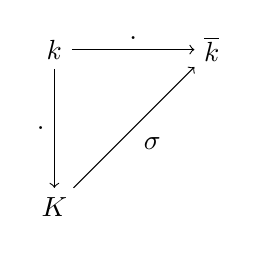
\begin{tikzpicture}[node distance=2cm, auto]
		\node (k) {$k$};
		\node (kk) [right of=k] {$\overline{k}$};
		\node (K) [below of=k] {$K$};

		\draw[->] (k) to node {$.$} (kk);
		\draw[->] (k) to node[swap] {$.$} (K);
		\draw[->] (K) to node[swap] {$\sigma$} (kk);

	\end{tikzpicture}
	\end{figure}

	\item $K$ é corpo de raízes sobre $k$ de uma família $(f_i)_{i \in I}$ de polinômios em $k[x] \setminus k$;
	\item Se $f \in k[x] \setminus k$ é irredutível em $k[x]$ com raiz $\alpha$, então $f(x)=c(x-\alpha_1)\cdots(x-\alpha_n)$ em $k[x]$, com $\alpha_1=\alpha$ e $c \in k \setminus \{0\}$.
	\end{enumerate}
\end{theorem}
%\begin{proof}
%PULEI, tem nas notas mas não tudo.
%\end{proof}

\begin{definition}
	Uma extensão de corpos $k \subseteq K$ é uma \emph{extensão normal} se ela satisfaz uma das três condições do teorema acima.
\end{definition}

OBS: Se $k \subseteq \overline{k}$ é uma extensão algébrica, então todo $\beta \in \overline{k}$ é algébrico sobre $k$ vale para $\beta \in K$, então $k \subseteq K$ é extensão algébrica.

	Se $k \subseteq K$ é extensão algébrica, então $k \subseteq K \subseteq \overline{K}$ são extensões algébricas, então $k \subseteq \overline{K}$ é extensão algébrica. Então $\overline{k} \sim \overline{K}$ é fecho algébrico de $k$.

%(?????)

\begin{proposition}
	Seja $k \subseteq K$ um extensão algébrica e $\sigma: K \to K$ um homomorfismo de corpos que satisfaz $\sigma|_k=id|_k$. Então $\sigma$ é um isomorfismo de corpos.
\end{proposition}
%\begin{proof}
%...
%\end{proof}

\begin{definition}
	Seja $E \subseteq F$ uma extensão algébrica e $\sigma:E \to L$ um homomorfismo de corpos tal que $L$ é algebricamente fechado, $\sigma(E) \subseteq L$ é uma extensão algébrica ($L$ é fecho algébrico de $\sigma(E)$)
	\begin{equation*}
	S_\sigma := \{\mu : \mu: F \to L \text{\ homomorfismo de corpos}, \mu|_E=\sigma\}.
	\end{equation*}
\end{definition}

\begin{lemma}
	$|S_\sigma|$ depende de $E \subseteq F$, mas não depende de $\sigma$ nem de $L$.
\end{lemma}
%\begin{proof}
%... vários diagramas
%\end{proof}

\begin{definition}
	Seja $E \subseteq F$ uma extensão algébrica. O \emph{grau de separabilidade} da extensão é $[F:E]_S := |S_\sigma|$. (Pode escolher $l=\overline{E}$ e $\sigma$ inclusão.)
\end{definition}

\begin{theorem}
	\begin{enumerate}
	\item $E \subseteq F \subseteq K$ extensões algébricas, então
		\begin{equation*}
		[K:E]_S = [K:F]_S[F:E]_S
		\end{equation*}
	\item $E \subseteq F$ extensão finita (logo algébrica), então
		\begin{equation*}
		[F:E]_S \leq [F:E]
		\end{equation*}
	\end{enumerate}
\end{theorem}
%\begin{proof}
%...
%\end{proof}

\begin{definition}
	Seja $E \subseteq K$ uma extensão finita. Ela é \emph{separável} se $[K:E]_S=[K:E]$.
\end{definition}

\begin{corollary}
	Sejam $E \subseteq F \subseteq K$ extensões de corpos, $[K:E] < \infty$, $E \subseteq K$ separável. Então $E \subseteq F$ e $F subseteq K$ são separáveis.
\end{corollary}
\begin{proof}
	\begin{equation*}
	[K:F]_S [F:E]_S = [K:E]_S = [K:E] = [K:F][F:E].
	\end{equation*}
	Como $[F:E]_S \leq [F:E]$ e $[K:F]_S \leq [K:F]$, segue o corolário.
\end{proof}



\section{Ação de anel}
\label{sec:aneis.acao}

Consideramos brevemente ações de anéis em grupos comutativos. Na definição usamos o fato de que, se $\bm G$ é um grupo comutativo, $\Homo(\bm G)$ é um anel com as operações puxadas para o espaço de funções, a soma pontual sendo a soma do anel e a composição de função sendo o produto. De fato, se $X$ é um conjunto e $\bm G$ um grupo comutativo, o conjunto $\Func(X,G)$ de funções de $X$ para $G$, com a soma pontual e a composição, é um anel, e basta mostrar que quando $X=G$, o conjunto $\Homo(\bm G)$ de endomorfismos de grupo de $\bm G$ é um subanel de $\Func(G)$.
Demonstramos isso a seguir.

\subsection{Anel de endomorfismos de grupo}

\begin{proposition}
Sejam $X$ um conjunto e $\bm G$ um grupo comutativo. Então
	\begin{equation*}
	\bm{\Func}(X,\bm G) := (\Func(X,G),+,-,0,\circ,\Id)
	\end{equation*}
é um anel\footnote{No sentido em que a multiplicação $\circ$ não precisa ser comutativa.}.
\end{proposition}
\begin{proof}
	\begin{enumerate}
	\item $(\Func(X,G),+,-,0)$ é um grupo comutativo.
		\begin{enumerate}
		\item Para todos $f_0,f_1,f_2 \in \Func(X,G)$ e $x \in X$,
			\begin{align*}
			((f_0+f_1)+f_2)(x) &= (f_0+f_1)(x)+f_2(x) \\
				&= (f_0(x)+f_1(x))+f_2(x) \\
				&= f_0(x)+(f_1(x)+f_2(x)) \\
				&= f_0(x)+(f_1+f_2)(x) \\
				&= (f_0+(f_1+f_2))(x);
			\end{align*}
		\item Para todos $f \in \Func(X,G)$ e $x \in X$,
			\begin{align*}
			(0+f)(x) &= 0(x)+f(x) \\
				&= 0+f(x) \\
				&= f(x) \\
				&= f(x)+0 \\
				&= f(x)+0(x) \\
				&= (f+0)(x);
			\end{align*}
		\item Para todos $f \in \Func(X,G)$ e $x \in X$,
			\begin{align*}
			((-f)+f)(x) &= (-f)(x)+f(x) \\
				&= -f(x)+f(x) \\
				&= 0 \\
				&= f(x)+(-f(x)) \\
				&= f(x) + (-f)(x) \\
				&= (f+(-f))(x);				
			\end{align*}
		\item Para todos $f_0,f_1 \in \Func(X,G)$ e $x \in X$,
			\begin{align*}
			(f_0+f_1)(x) = f_0(x)+f_1(x) = f_1(x) + f_0(x) = (f_1+f_0)(x).
			\end{align*}
		\end{enumerate}
	
	\item $(\Func(X,G),\circ,\Id)$ é um monoide.
		\begin{enumerate}
		\item Para todos $f_0,f_1,f_2 \in \Func(X,G)$ e $x \in X$,
			\begin{align*}
			((f_0 \circ f_1) \circ f_2)(x) &= (f_0 \circ f_1)(f_2(x)) \\
				&= (f_0(f_1(f_2(x))) \\
				&= f_0((f_1 \circ f_2)(x)) \\
				&= (f_0 \circ (f_1 \circ f_2))(x);
			\end{align*}
		\item Para todos $f \in \Func(X,G)$ e $x \in X$,
			\begin{align*}
			(\Id \circ f)(x) = \Id(f(x)) = f(x) = f(\Id(x)) = (f \circ \Id)(x).
			\end{align*}
		\end{enumerate}
	\item A composição $\circ$ é distributiva à esquerda e à direita sobre a soma pontual $+$.
		\begin{enumerate}
		\item Para todos $f,f_0,f_1 \in \Func(X,G)$ e $x \in X$,
			\begin{align*}
			(f \circ (f_0+f_1))(x) &= f((f_0+f_1)(x)) \\
				&= f(f_0(x)+f_1(x)) \\
				&= f(f_0(x))+f(f_1(x)) \\
				&= (f \circ f_0)(x) + (f \circ f_1)(x);
			\end{align*}
		\item Para todos $f_0,f_1,f \in \Func(X,G)$ e $x \in X$,
			\begin{align*}
			((f_0+f_1) \circ f)(x) &= (f_0+f_1)(f(x)) \\
				&= f_0(f(x)) + f_1(f(x)) \\
				&= (f_0 \circ f)(x) + (f_1 \circ f)(x).
			\end{align*}
		\end{enumerate}
	\end{enumerate}
\end{proof}

\begin{proposition}
Seja $\bm G$ um grupo comutativo. Então
	\begin{equation*}
	\bm{\Homo}(\bm G) := (\Homo(\bm G),+,-,0,\circ,\Id)
	\end{equation*}
é um anel\footnote{No sentido em que a multiplicação $\circ$ não precisa ser comutativa.}.
\end{proposition}
\begin{proof}
Como $\Homo(\bm G) \subseteq \Func(G)$, basta mostrar que $\Homo(\bm G)$ é subanel de $\bm{\Func}(\bm G)$.
	\begin{enumerate}
	\item $(\Homo(\bm G),+,-,0)$ é subgrupo.
		\begin{enumerate}
		\item Para todos $h_0,h_1 \in \Homo(\bm G)$ e $g_0,g_1 \in G$,
			\begin{align*}
			(h_0+h_1)(g_0+g_1) &= h_0(g_0+g_1) + h_1(g_0+g_1) \\
				&= h_0(g_0) + h_0(g_1) + h_1(g_0) + h_1(g_1) \\
				&= h_0(g_0) + h_1(g_0) + h_0(g_1) + h_1(g_1) \\
				&= (h_0 + h_1)(g_0) + (h_0 + h_1)(g_1);
			\end{align*}
		\item Para todos $h \in \Homo(\bm G)$ e $g_0,g_1 \in G$,
			\begin{align*}
			(-h)(g_0+g_1) &= -h(g_0+g_1) \\
				&= -(h(g_0)+h(g_1)) \\
				&= -h(g_0)-h(g_1) \\
				&= (-h)(g_0)+(-h)(g_1).
			\end{align*}
		\end{enumerate}
	\item $(\Homo(\bm G),\circ,\Id)$ é submonoide.
		\begin{enumerate}
		\item Para todos $h_0,h_1 \in \Homo(\bm G)$ e $g_0,g_1 \in G$,
			\begin{align*}
			(h_0 \circ h_1)(g_0+g_1) &= h_0(h_1(g_0+g_1)) \\
				&= h_0(h_1(g_0)+h_1(g_1)) \\
				&= h_0(h_1(g_0))+h_0(h_1(g_1)) \\
				&= (h_0 \circ h_1)(g_0)+h_0 \circ h_1)(g_1);
			\end{align*}
		\item Para todos $g_0,g_1 \in G$,
			\begin{align*}
			\Id(g_0+g_1) = g_0+g_1 = \Id(g_0)+\Id(g_1).
			\qedhere
			\end{align*}
		\end{enumerate}
	\end{enumerate}
\end{proof}

\begin{definition}
Sejam $\bm A$ um anel e $\bm G$ um grupo comutativo. Uma \emph{ação} de $\bm A$ sobre $\bm G$ é um homomorfismo de anel
	\begin{align*}
	\func{\bm \cdot}{A}{\Homo(\bm G)}{a}{
		\begin{aligned}[t]
		\func{a \bm \cdot}{G}{G}{g}{a \bm \cdot g}.
		\end{aligned}
	}
	\end{align*}
Denota-se $\acao{\bm \cdot}{\bm A}{\bm G}$. Diz-se que o anel $\bm A$ \emph{age} no grupo $\bm G$ e denota-se $\bm A \age \bm G$ se, e somente se, existe ação de $\bm A$ em $\bm G$.
\end{definition}

Se denotamos $\bm A=(A,+,-,0,\times,1)$ e $\bm G = (G,\bm +,\bm -, \bm 0)$, essa definição é equivalente às seguintes propriedades.
	\begin{enumerate}
	\item  Para todo $a \in A$, a função $\fun{a \bm \cdot}{G}{G}$ é um homomorfismo de grupo:
		\begin{enumerate}
		\item Para todos $a \in A$ e $g,g' \in G$,
			\begin{equation*}
			a \bm \cdot (g \bm + g') = a \bm \cdot g \bm + a \bm \cdot g'.
			\end{equation*}
		\end{enumerate}
	\item $\fun{\bm \cdot}{\bm A^+}{(\Homo(\bm G),\bm +,\bm -,\bm 0)}$ é homomorfismo de grupo:
		\begin{enumerate}
		\item Para todos $a,a' \in A$ e $g \in G$,
			\begin{equation*}
			(a + a') \bm \cdot m = a \bm \cdot g + a' \bm \cdot g;
			\end{equation*}
		\end{enumerate}
	\item  $\fun{\bm \cdot}{\bm A^\times}{(\Homo(\bm G),\circ,\Id)}$ é homomorfismo de monoide:
		\begin{enumerate}
		\item Para todos $a,a' \in A$ e $g \in G$,
			\begin{equation*}
			(a \times a') \bm \cdot g = a \bm \cdot (a' \bm \cdot g);
			\end{equation*}
		\item Para todo $g \in G$,
			\begin{equation*}
			1 \bm \cdot g = g.
			\end{equation*}
		\end{enumerate}
	\end{enumerate}